% This LaTeX document needs to be compiled with XeLaTeX.
\documentclass[10pt]{article}
\usepackage[utf8]{inputenc}
\usepackage{amsmath}
\usepackage{amsfonts}
\usepackage{amssymb}
\usepackage[version=4]{mhchem}
\usepackage{extpfeil}
\usepackage{stmaryrd}
\usepackage{graphicx}
\usepackage[export]{adjustbox}
\graphicspath{ {./images/} }
\usepackage{multirow}
\usepackage{fvextra, csquotes}
\usepackage{xeCJK}
\usepackage{polyglossia}
\usepackage{fontspec}
\usepackage{enumitem}
% 使用思源宋体 (衬线字体)
\setCJKmainfont{Noto Serif CJK SC}

% 或者,使用思源黑体 (无衬线字体)
% \setCJKmainfont{Noto Sans CJK SC}

% 或者,使用文泉驿微米黑
% \setCJKmainfont{WenQuanYi Micro Hei}

\setmainlanguage{english}
\IfFontExistsTF{CMU Serif}
{\setmainfont{CMU Serif}}
{\IfFontExistsTF{DejaVu Sans}
  {\setmainfont{DejaVu Sans}}
  {\setmainfont{Georgia}}
}


%New command to display footnote whose markers will always be hidden
\let\svthefootnote\thefootnote
\newcommand\blfootnotetext[1]{%
  \let\thefootnote\relax\footnote{#1}%
  \addtocounter{footnote}{-1}%
  \let\thefootnote\svthefootnote%
}

%Overriding the \footnotetext command to hide the marker if its value is `0`
\let\svfootnotetext\footnotetext
\renewcommand\footnotetext[2][?]{%
  \if\relax#1\relax%
    \ifnum\value{footnote}=0\blfootnotetext{#2}\else\svfootnotetext{#2}\fi%
  \else%
    \if?#1\ifnum\value{footnote}=0\blfootnotetext{#2}\else\svfootnotetext{#2}\fi%
    \else\svfootnotetext[#1]{#2}\fi%
  \fi
}

\begin{document}
\section*{内容简介}
这是一本自用逻辑学书籍。力求用简明有逻辑的语言将逻辑学的各个方面梳理清楚。
\section*{第一部分:逻辑与语言}

\section{逻辑学的基本概念}

\subsection{什么是逻辑学}
\textbf{逻辑学}是研究用于区分\textbf{正确推理}与\textbf{不正确推理}的\textbf{方法和原理}的学问。正确推理的界定有着许多客观标准,而如果不了解这些标准,也就无法运用它们。逻辑学研究的\textbf{宗旨},就是\textbf{发现并塑述这些标准},使之能够\textbf{检验论证},并\textbf{把好的论证与坏的论证区别开来}。

逻辑学家所关心的推理遍及\textbf{所有领域}:科学与医药,伦理与法律,政治与商务,运动与博弈,直至平凡的日常生活。其中所使用的多种多样的推理,都是逻辑学家感兴趣的。本书将要分析的大量论证,就涉及许多非常不同的领域。但我们所关心的不是这些论证的题材,而始终是它们的\textbf{形式(form)与品质(quality)},目的在于\textbf{学会如何检验与评价论证}。

逻辑学家并不关心推理的\textbf{思想过程},而只关心这种过程的\textbf{结果},即\textbf{论证}。论证是推理的\textbf{产品},可以被完整地写出来,并予以检验与分析。对逻辑学家来说,就每一个论证都可提出如下关键问题:
\begin{itemize}
    \item 论证所得出的\textbf{结论}是从论证所使用的\textbf{前提或假定}推出的吗?
    \item 论证的\textbf{前提}能够为接受其\textbf{结论}提供\textbf{良好的理由}吗?
\end{itemize}
如果论证的前提的确能够为接受结论提供\textbf{充分的根据},也就是说,如果断定前提为真就能够\textbf{保证}可断定结论为真,那么其所使用的\textbf{推理就是正确的},否则就是\textbf{不正确的}。

不能说只有学了逻辑学才能进行良好的或正确的推理,正如不能说只有学了生理学的运动员才能跑得快一样。并不懂得发生在其身体上的\textbf{实际过程}的运动员经常有出色的表现,而有些学习生理学的优等生,尽管有许多关于身体机能方面的知识,但在运动场上却难有作为。同样,\textbf{学了逻辑学并不能确保能够进行正确的推理}。

然而,一个学了逻辑学的人,比之一个从未思考过推理原理的人,其\textbf{进行正确推理的可能性要大得多}。这首先因为学习逻辑学可以习得许多\textbf{检验推理正确性的方法},能够\textbf{更容易地识别推理错误},从而使这些错误不容易在推理中滞留。在这些被识别出的错误中,有些普通的\textbf{推理谬误},或所谓的\textbf{“自然”错误},是只要把它们充分弄清就很容易避免的。

学习逻辑学能够\textbf{提高人的推理素养的另一个原因}是:它给了人们\textbf{训练(practice)分析论证以及建构自己的论证}的一种机会。推理是一种我们不但要\textbf{懂}而且要\textbf{做(do)}的事情,因而其\textbf{既属科学亦属艺术},需要\textbf{把握技术和开发技能}。就此目标,本书提供了丰富的习题训练,以增强这种技术与技能。

在人类生活中,有些事情并不能完全用逻辑方法加以分析,有些问题并不能用论证(即使是良好的论证)来解决。有时求助于情感比逻辑论证更有效力,在某些语境中或许也更为适当。但是,在那些必须依靠下判断的地方,\textbf{正确推理终究是其最坚实的基础}。运用逻辑学的方法与技术,人们可以\textbf{有效地区分正确的推理与不正确的推理},这种\textbf{方法与技术就是本书的主题}。


\subsection{命题与语句}
任何论证都是由\emph{命题}(proposition)构成的,故我们从讨论命题入手。
\textbf{命题是一种可以被肯定或否定的东西。}
也就是说,命题不同于问题、命令和感叹。问题可以被提问,命令可以被下达,感叹可以被发出,但它们本身都不能被肯定或否定。唯有命题断定了事情是(或不是)如此这般,因而也唯有命题才会是真的或者是假的。
\emph{真}(true)与\emph{假}(false)这两个值并不适用于问题、命令或感叹。

再者,任一命题必是\emph{或真或假}的,尽管我们可能并不知道某一特定命题究竟是真的还是假的。例如,命题:
\begin{quote}
    “宇宙中其他星球上有生命存在”
\end{quote}
就是一个我们迄今还不知道其真假的命题。但对地球外生命之存在的这种断定本身或者是真的,或者不是真的。简言之,\textbf{或真或假是命题的一个基本特征}。

依学界惯例,需要把\emph{命题}与用来表达命题的\emph{语句}(sentence)区别开来。两个由不同语词以不同方式组成的语句,可能在同一语境中具有同样的意义,被用来表达同一个命题。例如下面这两个语句:
\begin{itemize}
    \item \textit{Leslie won the election.} (莱斯利赢了这场选举。)
    \item \textit{The election was won by Leslie.} (这场选举由莱斯利赢得。)
\end{itemize}
这显然是两个不同的语句:前一个由四个词组成,后一个是六个词,且起首词也不同。然而,这两个陈述句无疑具有相同的意义,它们表达了\textbf{同一个命题}。命题这个术语所指谓的就是人们通常使用陈述句所断定的内容。

再者,一个\emph{语句}总是某个特定语言的语句,而\emph{命题}本身并不专属于任何特定语言。同一个命题可以在许多不同语言中被断定。例如,以下四个不同语言的语句都表达了同一个“天在下雨”的命题:
\begin{itemize}
    \item \textit{It is raining.} (英语:天在下雨。)
    \item \textit{Está lloviendo.} (西班牙语:天在下雨。)
    \item \textit{Il pleut.} (法语:天在下雨。)
    \item \textit{Es regnet.} (德语:天在下雨。)
\end{itemize}
这四个语句虽然分属英语、西班牙语、法语和德语,但它们都具有同样的意义,因而都可以用来断定同一个命题。

在不同的\emph{语境}(context)中,同一个语句也可能被用来做非常不同的\emph{陈述}(statement),即表达不同的命题。例如,考虑语句:
\begin{quote}
    “美国最大的州曾经是一个独立的共和国。”
\end{quote}
如果在 20 世纪上半叶说出这个语句,它陈述的是关于得克萨斯州的一个\emph{真}命题;而如果在今天(例如21世纪)说出,它陈述的则是关于阿拉斯加州的一个\emph{假}命题。显然,时间语境的变化,可以使完全相同的语句断定非常不同的命题。
(值得注意的是,“命题”和“陈述”这两个术语并不完全同义,但在逻辑研究的文本中它们经常被用作同义词。有些逻辑学专家更喜欢使用“陈述”而不愿意使用“命题”,但在逻辑学历史上后者更为常用。本书将同时使用这两个术语。)

上面所举出的命题的例子,如“莱斯利赢了这场选举”和“天在下雨”,都是\emph{简单命题}(simple proposition)。然而,命题也经常是\emph{复合命题}(compound proposition)——即在一个命题中包含着其他命题。考虑如下这段关于1945年希特勒第三帝国末日的描述性文字:
\begin{quote}
美军与俄军正迅速赶往易北河会师。英军已兵临汉堡和不来梅城下,把占领丹麦的德军置于被切断后路的险境。意大利的波伦亚已经失守,而亚历山大率领的盟军部队正向波河流域挺进。俄军已于4月13日攻克维也纳,正沿着多瑙河乘胜前进。${ }^{[1]}$
\end{quote}
这段话中就含有若干复合命题。例如,“英军已兵临汉堡和不来梅城下”这一命题,就是“英军已兵临汉堡城下”与“英军已兵临不来梅城下”这两个命题的\emph{联言式}(conjunctive form)。而这个\emph{联言命题}(conjunctive proposition)本身又作为分支,属于一个更大的联言命题,即文中所述的:“英军已兵临汉堡和不来梅城下,(英军)把占领丹麦的德军置于被切断后路的险境。” 这段话中的每一个命题都是被肯定的,也就是说,都被断言为真。肯定两个命题的联言式(或联言命题),就等于同时肯定这两个作为其分支的命题。

但是,也有一些复合命题并不断定其所有分支命题的真假。例如,考虑以下\emph{选言命题}(disjunctive proposition),亦称\emph{析取命题}:
\begin{quote}
    “巡回法庭或者是有用的,或者是无用的。”${ }^{[2]}$
\end{quote}
这个命题并没有肯定其任何一个分支命题(即“巡回法庭是有用的”或“巡回法庭是无用的”),而只是肯定了整个复合的“或者—或者”析取命题为真。当一个析取命题为真时,其某个分支命题可以为假。

再如,考虑以下\emph{假言命题}(hypothetical proposition),亦称\emph{条件命题}(conditional proposition):
\begin{quote}
    “如果上帝不存在,则有必要捏造一个上帝。”${ }^{[3]}$
\end{quote}
这个复合命题同样没有肯定其任何分支命题的真假:它既没有肯定“上帝不存在”,也没有肯定“有必要捏造一个上帝”。它只是通过这种假言或条件陈述肯定了整个“如果—则”命题的真实性。即使其分支命题均为假,整个条件陈述也仍然可以为真。

本书将逐次分析多种简单命题和复合命题的内在结构。

\subsection{论证、前提与结论}
命题是构成论证的部件。\emph{推论}(inference)这个术语则指谓以一个或更多命题作为出发点,得出另一命题的过程。逻辑学家即通过检验这种过程的出发点与结果及它们之间的关系,以判定一个推论是否正确。这种命题系列即构成一个\emph{论证}(argument)。因而对于任一可能的推论,都有一个相应的论证。

论证是逻辑学所关心的主要对象。逻辑学家所使用的“论证”一词,特指任一这样的命题组:其中一个命题是从其他命题推导出来的,而后者为前者之为真提供支持或根据。当然,“论证”一词也经常在其他含义上使用,但在逻辑学中严格地限于上述含义。

显然,在这种严格含义上,一个论证不只是一组命题的汇集;一段仅仅包含一些相互关联的命题的话语,可能并不包含任何论证。若要构成一个论证,该命题系列必须具有特定的结构,对这种结构的描述通常要使用\emph{前提}(premise)与\emph{结论}(conclusion)这两个术语。一个论证的\textbf{结论},就是以论证中的其他命题为根据所得出的那个命题;而这些其他命题,即被肯定(或假定)为接受结论的根据或理由的命题,则是该论证的\textbf{前提}。

最简单的论证是由一个前提和一个从该前提推出或被它所蕴涵的结论构成的论证。这种论证的前提与结论可以分别用两个不同的语句表述,例如出现在阿拉巴马州地理课本封签中的如下论证:
\begin{quote}
在地球上最先出现生命时没有人存在。因此,任何关于生命起源的陈述都应视为理论的而非事实的陈述。
\end{quote}
最简论证的前提和结论也可能被表述在同一个句子中,如下述论证:
\begin{quote}
因为最近的进化史研究已经证明所有人都是从同一小群非洲祖先演变而来,若仍相信种族间有极大差异,则如同仍相信地球是扁平的一样荒谬可笑。
\end{quote}
即使在最简论证中,结论陈述也有可能出现在那个唯一的前提之前。这时候,两个命题同样既可以以两个语句出现,亦可在同一个句子中出现。前者例如:
\begin{quote}
食品与药物管理局应立即禁止烟草买卖。要知道,抽烟是导致死亡的一种最可预防的原因。${ }^{[5]}$
\end{quote}
结论在前,且前提与结论表述于同一语句中的一个例子是:
\begin{quote}
凡法皆恶,乃因凡法皆为自由之违背。${ }^{[6]}$
\end{quote}
大多数论证都比这些例子复杂得多。我们将会看到,有些非常复杂的论证包含由多个支命题构成的复合命题。但是不管简单还是复杂,\textbf{任何论证都是由一组命题构成,其中一个命题是结论,其他命题是用以支持结论的前提}。

因为一个论证由一组命题构成,故而单一命题自身不可能是论证。但有些复合命题与论证非常近似,需细心辨识以免把它们混同于论证。考虑如下假言命题:
\begin{quote}
如果火星在其具有与地球相似的大气层和相似气候的早期曾有生命演化, 那么目前科学家确信的在我们的星系中存在的无数颗其他星球上也会有生命演化。
\end{quote}
在这个假言命题中,无论第一个支命题“火星在其具有与地球相似的大气层和相似气候的早期曾有生命演化”,还是第二个支命题“目前科学家确信的在我们的星系中存在的无数颗其他星球上也会有生命演化”,都没有被肯定。整个命题肯定的只是前者蕴涵后者,而两者却可以都是假的。其中没有推论得以构成,没有结论被断言为真。这是一个\emph{假言命题},而不是一个论证。

现再请考虑如下段落:
\begin{quote}
看来,目前科学家确信的在我们的星系中存在的无数颗其他星球上会有生命演化,因为火星在其具有与地球相似的大气层和相似气候的早期非常可能曾有生命演化。${ }^{[7]}$
\end{quote}
此处我们的确得到一个论证。命题“火星非常可能曾有生命演化”被肯定为一个前提,而命题“无数颗其他星球上会有生命演化”被从该前提推出并被断言为真。这样,假言命题可能看上去很像一个论证,但其并不是一个论证,两者不应混淆。如何识别论证,是后面 1.5 节讨论的主题。

最后应强调指出,任一论证都是有结构的命题系列,但并非任一有结构的命题系列都是论证。请考虑从近期的非洲游记上摘录的一段话:
\begin{quote}
骆驼并不在驼峰中储水。它们每次喝水都非常猛,在十分钟的时段中能饮入 28 加仑水,把这些水均匀地分布到全身。而后其耗水却非常节俭。它们的尿液黏稠、粪便干燥,呼吸徐缓,且通常紧闭其口以减少水分蒸发。如非不得已,它们一般不出汗……在失水程度达到体重的三分之一时也能存活,然后再痛饮一次并且感觉良好。${ }^{[8]}$
\end{quote}
这段有结构的命题系列中并没有任何论证。

\subsubsection{练习题}
\subsubsection*{下列各段话中均只含有一个论证,请指出其前提与结论。${ }^{[9]}$}

\subsubsection*{例题}
% Make sure the enumitem package is loaded, e.g., \usepackage{enumitem}
% The following line caused the error, changed . to .
\begin{enumerate}[label=\arabic*., itemsep=1ex, topsep=1ex]
\item 管理得当的民兵组织对于一个自由国家的安全是必需的,因而人民保存和持有武器的权利不得侵犯。\\
    \null\hspace{\parindent}-\textit{The Constitution of the United States, Amendment 2}
\end{enumerate}

\subsubsection*{解答}
前提:管理得当的民兵组织对于一个自由国家的安全是必需的。\\
结论:人民保存和持有武器的权利不得侵犯。

% Make sure the enumitem package is loaded, e.g., \usepackage{enumitem}
% The following line caused the error, changed . to .
\begin{enumerate}[label=\arabic*., itemsep=1ex, topsep=1ex, start=2]
\item 我们可以预防大多数癌症,即使我们不能直接找到这些癌症的原因;癌症的预防研究比治疗研究更显重要。\\
    \null\hspace{\parindent}-Daniel Callahan, \textit{"Lab Games", New York Times Book Review}, 9 April 1995
\item 良知(good sense),是这个世界分配得最均匀的东西。因为人人都认为自己具有非常充分的良知,就连那些在其他一切方面全都极难满足的人,通常也不会觉得自己的良知不够而想要再多得一点。\\
    \null\hspace{\parindent}-René Descartes, \textit{A Discourse on Method}, 1637
\item 在我们所有热情和欲望中,权力之爱是我们的专横和孤僻本性的表现,因为一个人的自尊心需要以公众对他的折服来满足。\\
    \null\hspace{\parindent}-Edward Gibbon, \textit{The Decline and Fall of the Roman Empire}, vol. 1, chap. IV
\item[*5.] 不要去审判别人,因为我们都是罪人。\\ % Custom labels like this are generally fine
    \null\hspace{\parindent}-William Shakespeare, \textit{Henry VI, Part II}, act 3, scene 3
\item 在为2000年全国人口普查做准备时,在美国宪法是否要求有一个点人头的实际人口数字的问题上,或者在用一种高级的抽样调查方法取代点人头法是否更适当的问题上存在着激烈的争论。1998年9月6日一封给《纽约时报》的来信中包含如下的论证:用“点人头”的方法,人口调查局不可能点清所有的美国人。因此“点人头”法本身也只是一种抽样统计法,其样本就是实际返回调查表的那部分人口。\\
    \null\hspace{\parindent}-----Keith Bradley, \textit{"What Did the Founders Expect From the Census?"}
\item 我们令人赞美的经济体制的本质是快速地创造人们的需求,其速度与该体制满足人们需求的速度一样快,或者更快。因此如果把改善生活条件定义为更大的消费满足的话,那么改善生活条件是不可能做到的。\\
    \null\hspace{\parindent}-J. Maher, \textit{"Never Better", New York Times}, 1 January 1993
\item 由于它们既给生化病原体扫清道路,又给生化病原体提供免费的交通工具,蜱是世界上一种最有害的传病媒介。\\
    \null\hspace{\parindent}-Cynthia Mills, \textit{"Blood Feud", The Sciences}, April 1998
\item 没有爱心的,就不认识神;因为神就是爱。\\
    \null\hspace{\parindent}-1 John 4:8
\item[*10.] 因为光以特定速度运行,所以看到数百万英里以外的物体实际上就是看到很多年前发出的光。\\
    \null\hspace{\parindent}--D. Richstone, \textit{"University of Michigan Joins Magellan Project", Ann Arbor News}, 13 February 1996
\item 禁止人们复制一本书并将复制品送给好友,尽管不是最好的办法,但却是合乎逻辑的;给你的朋友买一本平装本的书是很容易的,而且花费也不多。\\
    \null\hspace{\parindent}---Randy Cohen, \textit{New York Times Magazine}, 26 March 2000
\item 有些人活到 100 岁,却对人类的进步无所贡献;有些人殁于年轻,却建功于促进人类发展的事业。所以致力于延长人类寿命的科学手段的研究完全是不合理的。\\
    \null\hspace{\parindent}-William J. Cousins, \textit{"To a Long Life! But How Long?", New York Times}, 25 December 1999
\item 我们的论点(20 世纪70年代堕胎的合法化实际上减少了 20 世纪90 年代的犯罪)的理论辩护依据两个简单的假设:1)合法的堕胎导致更少“多余”婴儿的出生,2)多余婴儿更容易受到虐待和忽视,因此在以后的生活中更容易卷入犯罪。\\
    \null\hspace{\parindent}--Steven Levitt, \textit{www.slate.com/dialogues/}, 23 August 1999
\item 今天的大学一年级学生与 50 年前的同龄人相比,在外表上显得早熟多年。因此,传统上我们在大学时代才能领悟的一些事情,现在一定发生在中学里面。\\
    \null\hspace{\parindent}--Leon Botstein, \textit{Jefferson's Children: Education and the Promise of American Culture}, 1998
\item[*15.] 从事公共教育的学校乃因其自身的失败而兴旺。其学生表现越差,它从公众和政府那里要求(和得到)的钱就越多。它得到的钱越多,它自身发展得就越快。\\
    \null\hspace{\parindent}--Ian Hamet, \textit{"School for Scandal", The Weekly Standard}, 23 August 1999
\item 对于魔术师而言,理想的观众是数学家、哲学家和科学家。因为他们的逻辑头脑对显明的因果联系接受很快,当幻觉达到“不合逻辑”的顶点时,他们更易于感到惊奇。\\
    \null\hspace{\parindent}-Martyn Bedford, \textit{The Houdini Girl}, Pantheon Books, 1999
\item (对性骚扰的)起诉基于“影响”而不是意图;因此如果起诉者相信被告是有罪的,他就是有罪的。\\
    \null\hspace{\parindent}--Herbert London, New York University Dean, quoted in Alan Kors and Harvey Silverglate, \textit{The Shadow University}, The Free Press, 1998
\item 当人们活着时,根据他们的收入征税;当人们死了并把他们一生的积蓄传给他们的儿女、孙儿女或他们选择的慈善机构时,就对他们加倍征税,这是错误的。死亡税,或称遗产税,是不公平的,应当取消。\\
    \null\hspace{\parindent}--Representative Bill Archer, Chairman of the U.S. House Committee on Ways and Means, 3 July 1998
\item 标准化考试对于不同人种和少数民族学生有着根本不同的影响。白人和亚洲学生的平均成绩明显高于他们的黑人和拉丁美洲籍同学。对于四年级考试、大学入学考试以及对书本知识的其他各种考试而言,这都是事实。如果这种种族间差距是种族歧视的证据,那么所有考试就都存在种族歧视。\\
    \null\hspace{\parindent}-Abigail Thernstrom, \textit{"Testing, the Easy Target", New York Times}, 15 January 2000
\item[*20.] 无疑,今天的医学研究没有比研制艾滋病疫苗更重要的目标了。去年(1998 年),由 HIV(人类免疫缺乏病毒)引起的艾滋病是死亡率最高的传染病,并且艾滋病的蔓延趋势没有减缓。\\
    \null\hspace{\parindent}-David Baltimore, President of the California Institute of Technology in \textit{The Chronicle of Higher Education}, 28 May 1999
\end{enumerate}

\subsection{论证的分析}
许多论证是简单的,但有些论证却相当复杂。论证的前提可以用各种不同方式支持其结论。论证中前提的数量和命题顺序也有所不同。我们需要关于论证性话语的一些分析技法,借以澄清前提与结论的关联。

通常有两种分析技法用于论证分析。一种是解析(paraphrase),即 12用清楚的语言和逻辑顺序表明论证中的命题;另一种是图示(diagram),用二维空间关系图展示论证的结构。两种技法都很有用,可根据不同情况选用最方便适用的一种。

\subsection{A.解析法}
考虑下面这个多于两个前提的论证的原初表述:

现代鸟类并非从直立行走的兽脚类恐龙(包括霸王龙)进化而来,有三个主要理由。首先,大多数类鸟兽脚类恐龙化石发源时间比初始鸟类遗留的化石晚七千五百万年。……其次,鸟的祖先必定已适宜飞行,而兽脚类恐龙并不适宜飞行。第三个理由在

于...…兽脚类恐龙都有锯状牙齿,而鸟类没有锯状牙齿。 ${ }^{[10]}$

我们可通过解析澄清该论证,即利用清楚简明的语言列出其每一个前提及结论:

1.类鸟兽脚类恐龙化石比初始乌类遗留的化石发源时间要晚得多。\\
2.乌的祖先必定已适宜飞行,但兽脚类恐龙不适宜飞行。\\
3.兽脚类恐龙都有锯状牙齿,而鸟类没有锯状牙齿。\\
所以,现代鸟类并非从直立行走的兽脚类恐龙进化而来。

对论证的分析通常能帮助我们更好地理解论证,因为做这样的分析必须把在论证中被假定但没有充分明晰地陈述的东西揭示出来。辟如大数学家哈代曾有如下论说:

阿基米得将被永远记住而埃斯库罗斯会被遗忘,因为一种语言会消亡而数学理念不会消亡。 ${ }^{[11]}$

对该论证的充分的分析,需清楚地表明其所承诺的东西:

1.一种语言会消亡。\\
2.埃斯库罗斯的伟大剧作使用一种语言。\\
3.故埃斯库罗斯的成果终究会消亡。\\
4.数学理念不会消亡。\\
5.阿基米得的伟大工作使用数学理念。\\
6.故阿基米得的成果不会消亡。\\
所以,阿基米得将被永远记住而埃斯库罗斯将被遗忘。

这种分析使我们看到,哈代这一短句之中,浓缩了几个带有可疑前提的论证。

\subsection{B.图示法}
有时运用图示展示一个论证的结构是非常有益的。其步骤是给论证中

出现的每一个命题逐次赋予一个置于圆圈中的数字,然后在数字间使用箭头符号展示其中前提与结论的逻辑关联。这样可避免像解析法那样重述前提。考虑如下论证:\\
(1)与许多人的认识相反,HIV 检测呈阳性并不必定是死亡判决。一方面,(2)从(艾滋病病毒)抗体生发到出现临床症状平均将近十年时间;另一方面,(3)许多研究报告显示,相当数量的检测呈阳性者从未发展为艾滋病患者。 ${ }^{[12]}$

不用重述论证中的命题,使用标示命题的圆圈数字即可把该论证图示如下:\\
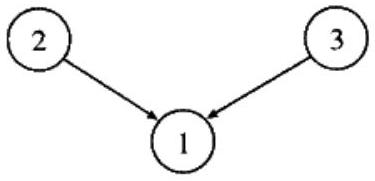
\includegraphics[max width=\textwidth, center]{2025_05_15_6a28331d5e7c993ad07ag-030}

如果一个论证是简单直接的,则完全不需要借助图示去理解它。然而论证往往不是直接的,而图示法能够在平面图上直观地显示论证的结构,因而是非常有用的。 ${ }^{[13]}$ 我们在图中把结论置于前提的下方,而论证的所有前提都在图中的同一行上列出。

与解析法相比,图示法更易于展现论证的前提支持结论的方式。例如在上面这个论证中,前提(2)和(3)都分别独立地支持结论(1):HIV 检测呈阳性并不必定是死亡判决。就是说,每个前提自身都为接受结论提供了某种理由,即使没有另一个前提也不影响其为结论所提供的支持。这种分立性支持直观地展现在图示之中。

但是,在有些论证中,只有把前提结合在一起才能达到支持结论的目的。例如:

该论证的正确图示将展现出只有当前提之间相结合才能支持结论,即:\\
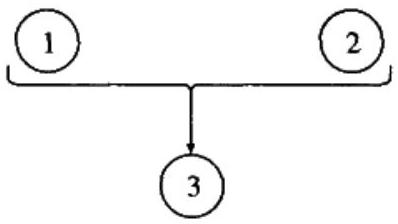
\includegraphics[max width=\textwidth, center]{2025_05_15_6a28331d5e7c993ad07ag-031(1)}

此处我们用托架线置于前提之下,是因为在这个例子中两个前提都不能独立地支持结论。如果第一个前提表达的原则是真的,但不存在能够最适当地维护所有当事人的利益的安乐死事例,则结论就根本没有得到支持。而如果的确存在能够最适当地维护所有当事人的利益的安乐死情形,但第一个前提所表述的原则是错误的,则结论仍然没有获得支持。

当论证有更复杂的结构时,图示法就显得特别有用。有时可以很容易地展示出原本很难说清楚的东西。考虑如下论证:

\begin{displayquote}
(1)沙漠高地是天文观测的良好场所。(2)其高度使得它们坐落于大气层之中,使得星光不用穿越整个大气层而到达望远镜。 (3)沙漠的千燥度也使之相对较少受云雾千扰。(4)云雾对天空的遮蔽会使许多天文观测归于无用。 ${ }^{[15]}$
\end{displayquote}

命题(1)显然是这个论证的结论,其他三个命题提供对它的支持,但它们支持结论的方式是不一样的。命题(2)自身即可支持沙漠高地是天文观测良好场所的断言,而命题(3)和(4)必须联合起来才能支持这个断言。如下图示可清楚地表明这一点:\\
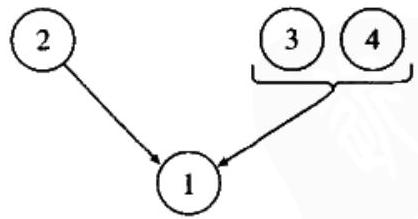
\includegraphics[max width=\textwidth, center]{2025_05_15_6a28331d5e7c993ad07ag-031}

但是某些复杂论证结构的澄清使用解析法更为奏效。例如,当一个论证含有未明确陈述出来的隐含前提时,解析法允许我们直接把隐含前提列出,而图示法则需要既列出隐含前提又要以某种直观形式(如非封闭圆圈)表明它是被附加到原来论说之上的。请考虑如下论证:

只有当我能够做出其他选择时,我对我的行为才负有道德责任。因为一个人若无力避免某行为,就不应被认为对该行为负有道德责任。 ${ }^{[16]}$

运用列出隐含前提的解析法,该论证很容易澄清如下:

1.一个人若无力避免某行为,就不应被认为对该行为负有道德责任。\\
2.只有当我能够做出其他选择时,我当下的行为才是我有能力避免的。所以,只有当我对我的行为负有道德责任时,才有我的行为是否应当的问题。

\section*{C.多重复合论证}
当一段话包含两个或更多论证和若干相互关联并不明显的命题时,图示法被证明特别有用。下面是从马克思给恩格斯的一封信中摘录的一段话:

\begin{displayquote}
(1)加速英国的社会革命就是国际工人协会的最重要的目标。(2)而加速这一革命的唯一办法就是使爱尔兰独立。因此, (3)国际的任务就是到处把英国和爱尔兰的冲突提到首要地位, (4)到处都公开站在爱尔兰方面。 ${ }^{[17]}$
\end{displayquote}

一段话中论证的数目通常取决于其中所含结论的数目。这段话中含有两个结论,因而有两个论证。但这两个结论都是从同样的两个前提推得的,如 16下图示可很好地展示这种结构:\\
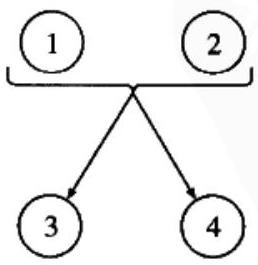
\includegraphics[max width=\textwidth, center]{2025_05_15_6a28331d5e7c993ad07ag-032}

有时,含有两个结论从而有两个论证的一段话,却只含有一个前提。例如:

年纪较大的妇女更难以抵制工作中的性骚扰和离开施暴的丈夫,因为年龄的偏见使她们不容易找到其他保护自己的方式。 ${ }^{[18]}$

其中唯一的前提是年纪较大的妇女不容易找到保护自己的方式。该前提支持两个结论:年纪较大的妇女难以抵制工作中的性骚扰,以及她们(对已婚妇女而言)难以离开施暴的丈夫。我们通常用"单独论证"一词指谓只有一个结论的论证,而不管有多少用以支持它的前提。

当一段话中出现两个或更多论证,或一个论证中有两个或更多前提时,就需要弄清各个前提及结论出现的次序。结论可能在最后或最先出现,也可能出现在用以支持它的前提之间,如下例:

移斯林思想家启示的真正来源是《古兰经》及神圣先知的言论。因而很显然,移斯林哲学并不是希腊思想的复制品,其所关心的主要是那些来自移斯林和与穆斯林相关的特定问题。 ${ }^{[19]}$

这段话中的结论"穆斯林哲学并不是希腊思想的复制品",出现在论证的第一个前提之后和第二个前提之前。

同一个命题既可在一个论证中做结论,又可在另一个论记 中做前提,正如同一个人既可在一个场合做指挥者,又可在另一个场合做被指挥者。托马斯-阿奎那的著作中有一段话可以很好地说明这一点。他说:

\begin{displayquote}
人类的法律是为人类大众制定的,\\
大多数人在德行上是不完美的,\\
因此人类的法律不禁止一切罪恶。 ${ }^{[20]}$
\end{displayquote}

17 该论证的结论随即被托马斯-阿奎那用做另一个完全不同的论证的前提:

\begin{displayquote}
恶行与善行相反,\\
但人类的法律不禁止一切罪恶,\\
因此人类的法律也不规定一切善行。 ${ }^{[21]}$
\end{displayquote}

以被压缩,对于这样一串浓缩论证的分析,完全解析法会提供很大的帮助。考虑如下论证集合:

因为(1)出现在非洲人种身上的线粒体变种最多,科学家推断,(2)非洲人种的进化史最长,这表明(3)非洲人种可能是现代人类的起源。 ${ }^{[22]}$

我们可以把这段论证图示如下:\\
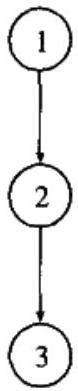
\includegraphics[max width=\textwidth, center]{2025_05_15_6a28331d5e7c993ad07ag-034}

而对这同一串论证的分析,解析法尽管显得不够简洁,但更完整:

1.一个人种身上的线粒体变种越多,其进化史就越长;\\
2.出现在非洲人种身上的线粒体变种最多,因此非洲人种进化史最长。

1.非洲人种进化史最长,\\
2.现代人类可能起源于进化史最长的人种,因此现代人类可能起源于非洲人种。

这样的复合论证表明,一个孤立表达的命题既非前提也非结论。在一个论证中,作为假定出现的命题就是前提,被断定为从假定命题推出的命题就是结论。也就是说,"前提"和"结论"都是相对的(relative)术语。

几个论证复合在一起,语言表达上可能不是以串联的方式出现,而是以独特的方式相互交织,这就要求我们对它们做细致的分析。图示法特别适用于这种情况。例如,在约翰•洛克的名篇《政府论》中,下面一段话

就有两个论证交织在一起:

立法机构常年运作是不必要的,也是很不方便的;但行政机关常年运作是绝对必要的,因为不是总需要制定新的法律,但总需要执行已制定的法律。

上述论证的分支命题可以用数字表示为:(1)立法机构常年运作是不必要的,也是很不方便的,(2)行政机关常年运作是绝对必要的,(3)不是总需要制定新的法律,(4)总需要执行已制定的法律。将这段论证图示如下:\\
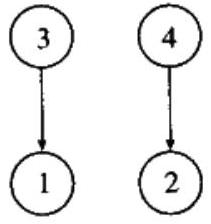
\includegraphics[max width=\textwidth, center]{2025_05_15_6a28331d5e7c993ad07ag-035}

这个图示表明,第二个论证的结论出现在第一个论证的结论和前提之间,第一个论证的前提出现在第二个论证的结论和前提之间。这个图示还表明,两个结论都出现在它们的前提之前。

这个图示同样也展示了支持刑罚威骤理论的古罗马哲学家塞涅卡的两个相关论证的逻辑结构:\\
(1)惩罚罪行不是因为罪行已经发生,(2)而是为了不发生新的罪行。[因为](3)过去的罪行不能被取消,(4)但是可以预防将来的罪行。

在这段话中,"惩罚罪行不是因为罪行已经发生"是其中一个论证的结论,其前提是"过去的罪行不能被取消"。"惩罚罪行是为了不发生新的罪行"是这段话中第二个论证的结论,其前提是"惩罚罪行可以预防将来的罪行"。

简言之,图示法和解析法是两种有力的分析工具,运用这两种工具对论证进行分析,可以更彻底地理解论证前提与结论的关联。

\subsubsection{练习题}
下列各段话涉及一些重要的公共政策问题,都选自近期的《纽约时

报》。请分析每段话中所含的论证,必要时对命题进行解释并图示论证。例题\\
1.基因和蛋白质是被发现的,不是被发明的。发明可以获得专利,发现不能。因此,蛋白质专利权本质上是有缺陷的。\\
-Daniel Alroy,"Invention vs.Discovery", New York Times, 29 March 2000

\subsubsection{解答}
前提:蛋白质是被发现的,不是被发明的。\\
发现不能获得专利,尽管发明能获得专利。\\
结论:蛋白质专利权本质上是有缺陷的。\\
2.为什么要反对财富差距?第一,不平等与政治不稳定相关联。第二,不平等与暴力犯罪相关联。第三,经济的不平等与期望寿命的减少相关联。第四个理由就是朴素的公正原则。最高行政长官的报酬是普通雇员的数百倍,这在道义上是没有正当理由的。\\
-Richard Hutchinsons,"When the Rich Get Even Richer",New York Times, 26 January 2000\\
3.股价正在下跌的华尔街把最近的就业数字视为通货膨胀率上升的新证据,即使不能视为立即上升的证据,也可以视为出现上升趋势的早期征兆。其所关注的是,雇员的短缺会迫使雇主给雇员支付更高的工资,然后用提高价格来弥补增加的劳动成本。\\
-Louis Uchitelle,"387000 New Jobs", New York Times, 5 February 2000\\
4.已婚者比独身者身体更健康,经济更稳定,婚生子女在各项指标上都做得更好。因此婚姻是一种负责任的社会行为。在税收法规里必须以某种方式贯彻对婚姻予以支持的原则。\\
--Anya Bernstein,"Marriage,Fairness and Taxes",New York Times, 15 February 2000\\
*5.如果你没有爱情而结婚,这并不意味着你以后不会逐渐爱上与你结婚的人。如果你与你所爱的人结了婚,这也不意味着你将永远爱这个人而有一个成功的婚姻。在许多由父母预先指定婚姻的国家,离婚率非常

低;而在人们根据爱情决定婚姻的国家,离婚率却非常高。\\
---Alex Hammoud,"I Take This Man,For Richer Only",New York Times, 18 Feb- ruary 2000

6.我们整个税收体系,依赖于绝大多数纳税人对于他们会受到公正的对待抱有信心,对于他们的竞争者和邻居也会支付其应付的税款抱有信心。如果公众得出结论:IRS(美国国内税收局)不能满足人们的这些基本期望,那么税收体系的风险将会变得很高,而这样的局面将很难逆转。\\
-David Cay Johnston,"Adding Auditors to Help IRS Catch Tax Cheaters",New York Times, 13 February 2000

7.自1976年以来,美国各州已经对 612 人执行了死刑,同时从死囚牢房中释放了 81 名被证明是清白无辜者。我们是否有理由相信我们的刑事司法体系在非死刑案件中有更高的准确率呢?如果我们的刑事司法体系在非死刑案件中的错判率达到死刑案件错判率的一半的话,那么就有数千无辜的人生活在我们的监狱中。\\
----Philip Moustakis,"Missing:A Death Penalty Debate",New York Times, 23 February 2000

8. 20 世纪 90 年代纽约州和得克萨斯州所走的截然不同的道路说明,过于依赖监狱作为消除犯罪的手段是无益的。得州在20世纪90年代被投人监狱的人数比纽约州全部在押人数(73233 人)多 98081 人。如果监狱能消除犯罪的话,从控制犯罪的观点来看,得州打击犯罪的力度远超过纽约州。但是从1990年到1998年,纽约州犯罪率的下降超过得州达 $26 \%$ 。\\
---Vincent Schiraldi,"Prisons and Crime", New York Times, 6 October 2000

9.在美国的多数总统选举中,超过半数的州是被忽视的。不生活在所谓摇摆州的投票人在四年一次的大选中实际上是旁观者。美国宪法修正案应当用直接选举制度取代陈旧的选举人选举制度。只有这样,所有 50个州的公民才能完全参加到选举我们国家领导人的活动中来。\\
-Lawrence R.Foster,"End the Electoral College",New York Times, 27 Septem- ber 2000\\
*10.按请愿人所论,国会就可以去控制任一对人们的就业、生产、运输和消费有实质的全国性影响的罪行。如果国会可以去控制性暴力犯罪 (基于其理由),它就可以,控制谋杀或其他任何种类的暴力犯罪,因为作为所有暴力犯罪中的一种类型,性暴力犯罪对经济的影响肯定小于其他大"部分种类的暴力犯罪。\\
----Chief Justice William Rehnquist,U.S. Supreme Court,U.S.v.Morrison,De- cided 15 May 2000\\
*11.供讨论:\\
在弗吉尼亚州最近的一次谋杀案审判中,法官指令陪审团:如果情况表明毫无疑问地至少具有下列两种严重事实之一,"你们就可以决定对被告处以死刑":或者被告将继续成为对社会的严重威胁,或者其罪行是 "残暴的或极端可耻的,恐怖的或丧失人性的"。在査明被告确实有罪以后,陪审团仔细研究如何判决,对法官提出这样的问题:如果我们相信情况符合两种严重事实之一,"那么发布死刑处罚令是我们陪审团的义务吗?"法官的回答仅仅是请他们重温就这一问题早已给出的指令。两个小时以后陪审团带着对这个被告的死刑判决回到法庭,其中有人含着眼泪。

这个死刑判决被上诉到联邦最高法院进行复审(Weeks v.Angelone, No.99-5746,decided 19 January 2000)。最高法院面临的争议是,在这个案件的背景下,是否应当以下达给陪审团的指令曾使陪审团感到困惑为理由而取消死刑判决。你将构建怎样的论证来支持争论的一方?

\subsection{1.5 论证的辨识}
\subsection{A.结论和前提指示词}
如前所见,出现在论证性话语中的命题的次序不能作为辨识其结论或前提的依据。那么用什么来辨识呢?有一些被叫做"结论指示词"的词或短语有助于这样的辨识,因为它们典型地适合引导出一个论证的结论。下

面所列的就是部分结论指示词 ${ }^{(1)}$ :

\begin{center}
\begin{tabular}{|l|l|}
\hline
therefore(所以) & for these reasons(基于这些理由) \\
\hline
hence(因此) & it follows that(可推得) \\
\hline
thus(因而) & we may infer(我们可推出) \\
\hline
so(故而) & I conclude that(我推断) \\
\hline
accordingly(由此可见) & which shows that(这表明) \\
\hline
in consequence(于是) & which means that(这意味着) \\
\hline
consequently(可得) & which entails that(据此可得) \\
\hline
proves that(据此证明) & which implies that(这蕴涵) \\
\hline
as a result(之所以) & which allows us to infer that(据此我们可以推出) \\
\hline
for this reason(为此缘故) & which points to the conclusion that (据此可得结论) \\
\hline
\end{tabular}
\end{center}

另一些词或短语典型地适合作为论证前提的标志,因而被叫做前提指示词。通常,但非总是,跟在任一前提指示词之后的命题就是某个论证的前提。下面所列的是部分前提指示词:\\
since(因为)\\
because(由于)\\
for(因)\\
as(根据)\\
follows from(从……推出)\\
as shown by(正如……所表明)\\
inasmuch as(缘于)

\section*{B.语境中的论证}
$$
\begin{aligned}
& \text { as indicated by (正如......所示) } \\
& \text { the reason is that (理由是) } \\
& \text { for the reason is that (理由在于) } \\
& \text { may be inferred from (可从.....推出) } \\
& \text { may be derived from (可从......引晴) } \\
& \text { may be deduced from (可从.....得出) } \\
& \text { in view of the fact that (有鉴于) }
\end{aligned}
$$

上面所列的词和短语可以帮助我们认识话语中所含的论证,辨识其前

\footnotetext{(1)下列英汉指示词并非一一对应,在自然语言中识别论证,主要应诉诸语境分析。一一译者注(以下凡脚注均为译者注,不一一标明)
}提或结论,但它们在实际论证中并不一定出现。论证的出现可以由话语的背景或意义来表明。例如,一个女作家用如下陈述对吸烟提出严厉的批评:

是否吸烟是在拥有关于烟草对健康的致命影响的充足信息的情况下做出的有意识的决定。无疑,那些对此做出不明智选择的人,应为其导致健康恶化的后果负责。 ${ }^{[23]}$

这段话中既没有前提指示词,也没有结论指示词,但其中所含的论证是很清楚的。同样,下面一段话中所包含的论证可以从其所含命题本身的意义辨识出来:

\begin{displayquote}
近年来,有关死刑处罚的威慑作用的论证受到人们的反驳。谋杀率最高的二十个州中的十八个州有死刑处罚。谋杀率最高的十七个大城市拥有死刑处罚的司法权。过去十年中,得克萨斯州处死的罪犯比其他任何一个州都多,但得州仍有三个城市的谋杀率列于谋杀率最高的二十五个城市之中。近二十年来,有两个接壤的州的谋杀率基本相当,一个是没有死刑处罚的密歇根州,另一个是有死刑处罚的印第安纳州。 ${ }^{[24]}$
\end{displayquote}

这些语段的论证性功能由它们的语境和它们的意义展现出来。这就好比当我说晚饭时带只龙虾回家,你不会怀疑我是打算吃掉而不是饲养它。

另一个没有结论或前提指示词的论证出现在最近一篇为比例代表制进行辩护的文章中:

单一成员选区(the single-member-district)的选举制度看来有许多严重的彎端。这种制度通常不能代表为数众多的选民的意志,它产生的立法机关不能准确反映公众的看法,它歧视第三党,挫伤选民投票的积极性。[25]

虽然可将这段话看做是首先陈述一个广泛的实际情况,然后用单一成员选 2.3区的选举制度的各种后果去阐明它,但也可以将这段话同样很好地理解为

一个首先陈述其结论,然后从支持这个结论的前提推出这个结论的论证。\\
下面一段最高法院关于公立学校反种族隔离问题的评判中,有一个既无结论指示词又无前提指示词的更复杂一些的论证:

\begin{displayquote}
在学生人数上存在种族不平衡的现象,这不等于表明乡村学校不履行其法律义务。种族平衡本身不是目的。若种族不平衡是由于违背宪法使然,必须予以追究。只要杜绝违法的种族不平衡,乡村学校并没有义务去纠正因人口因素而造成的种族不平衡。 ${ }^{[26]}$
\end{displayquote}

这段话的第一个句子是其所含论证的结论,这个结论可以被解释为"种族不平衡的存在并不表明乡村学校违背了法律"。我们怎么知道它是结论呢?这里语境是决定性的:接在第一个句子后面的几个句子提供了之所以如此的理由。我们看到,在第一个句子中所指谓的"乡村学校"的行为处于争论之中;后面的几个句子表达了几个与乡村学校的行为有关的更一般的命题。话语中所选用的语词也给出了线索,虽然短语"不等于表明"不是结论指示词,但它传达了这样一个暗示,即第一个句子是这段话的逻辑终点。

包含论证的语段经常含有一些既不能作为前提也不能作为结论的附加材料。有时那些提供背景信息的材料能使读者(或听者)理解论证是关于什么内容的。在下面这段话中,论证出现在最后一句中,但如果不抓住它前面句子的内容,这个论证就不可理解:

由于政府削减了对学生的财政援助,许多一流学院和大学都将较大比例的学费收入用做贫困学生的奖学金。正如慈善捐款可免征所得税一样,这部分学费也应亨受税务免征。 ${ }^{[27]}$

严格地讲,这段话中的第一个句子不是论证的一部分,但没有这句话我们就不能理解"这部分"学费是指用做奖学金的那部分学费。据此理解,我们就可以对该论证做如下解释:

1.对贫困者的慈善捐款是免征所得税的。

2.很大一部分学费收人被学校用来作为给贫困学生提供奖学金的慈善捐款。

所以,作为给贫困学生提供奖学金的那部分学费应免征所得税。

可见,上下文中命题之间相互参照,对于理解论证本身是必不可少的。哲学家阿瑟-叔本华在为自杀行为进行(无罪)辩护时所做的一个论证就例示了这种对相互参照的依赖:

\begin{displayquote}
如果罪法禁止自杀,那么在基督教中这并不是一个有根据的论证;而且这个禁令是荒唐的,因为有什么惩罚能让一个连死都不怕的人害怕呢?${ }^{[28]}$
\end{displayquote}

这段话分号前面的句子既非前提也非结论,但是若没有它,我们就不知道在随后出现的论证结论("这个禁令是荒唐的")中的"禁令"乃指谓罪法的自杀禁令。

\subsection{C.非陈述形式的前提}
在上一例子中,论证前提以疑问句的形式出现:"有什么惩罚能让一个连死都不怕的人害怕呢?"而正如 1.2 节所述,问题无所断定,不表达命题,那么一个疑问句何以能起到前提的作用呢?这取决于该问句是反诘问句。就是说,当提问者相信问题的答案显然或确定无疑时,可用问句暗示或设定一个前提。在上例中,叔本华认为他的问题的答案明显是"没有",因而,尽管以问句的形式出现,其论证的前提乃是这样一个不言而喻的命题:"没有任何惩罚能够让一个连死都不怕的人害怕。"

前提之一是反诘问句,而问题的答案被设定为明显的,这样的论证是非常普遍的,它们也很有修辞效果。可是这样使用问句是有风险的。例如苏格拉底的如下论证:

美诺啊,如果没有人欲望痛苦,那么就没有人欲望罪恶;因为除了欲望和拥有灾难,还有什么是痛苦的呢?[29]

严格地讲,其中的问句既不真也不假。如果设定为显然或确定无疑的答案

事实上并非如此,那么这个论证就是有缺陷的,而其缺陷正可能被问句掩盖。苏格拉底所假定的痛苦就是欲望和拥有罪恶这个答案是正确的吗?回答并不是显而易见的。

依赖反诘问句的论证,其结论有时是可疑的。人们使用设定有明显答案的问句来做论证的前提,有时就是为了回避直截了当地肯定其前提的责任,而实际上其设定的答案是含糊的甚或是假的。

不过,把真正的反诘问句作为前提使用确是一种很机敏的方法。通过暗示被期望的答案并且引导读者自己引出那个答案,可以增强论证的说服力。考虑下面两个使用反诘问句的例子。《新约全书》中有如下一段话:

\begin{displayquote}
人若说:"我爱神",却恨他的兄弟,就是说谎者:因为不爱他所看见的兄弟,如何能爱他看不见的神呢?[30]
\end{displayquote}

在最近的一篇对安乐死主张进行评论的文章中,有下面一段论证:

\begin{displayquote}
如果安乐死的权利基于自己的决定,那么将其限制到垂死病人就是不合情理的。如果人们有死亡权,那么为什么必须要等到已濒临死亡的时候才能行使这个权利呢?[31]
\end{displayquote}

在上面的两例论证中,两个设问的答案(一个是"不能爱他的兄弟的人也不能爱神",另一个是"人们不必要等到已濒临死亡的时候才能行使死亡权")都被假定是非常明显的。这些答案就是支持预期结论的前提。两个预期的结论分别是:"爱神的人不能恨他的兄弟"和"如果人们有基于自己决定的安乐死的权利,那么就不能将死亡权限制到垂死病人"。

有时论证的结论可以采用祈使句或命令句的形式。在给出劝说我们去采取一个特定的行动的理由后,我们被指导要如此这般地去行动。例如《箴言》(1)中有这样一句话:

\begin{displayquote}
智慧为首,所以要求得智慧。
\end{displayquote}

\footnotetext{(1)Proverbs,见《旧约全书》。
}在《哈姆雷特》中,波洛涅斯对他的儿子雷欧提斯提出如下忠告:

\begin{displayquote}
不要向人告贷,也不要借钱给人;\\
因为债坆放了出去,往往不但丢了本钱,而且还失去了朋友;
\end{displayquote}

向人告货的结果,容易养成因循懒惰的习惯。 ${ }^{[32]}$

因为命令句像一般疑问句一样不能表达命题,所以(严格来讲)命令句不能作为论证的结论。但是为简明计,我们可以把在这些语境中的命令句与命题同样对待,这是很有益处的。在这些语境中听者(或读者)被告知他们应当(should)或应该(ought to)以在命令句中已经说明的方式去行事。那么上面两个论证中的结论可以被解释为:"求得智慧是你应当去做的事情"和"你应该既不借钱给别人也不向别人告贷"。

几乎所有人都会同意,这种断言可以是或真或假的。如果在一个应当去做某事的命令和一个应当做某事的陈述之间有什么区别的话,这种区别恰恰是一个困难的问题,这个问题在这里不必探究。通过忽略这种区别 (如果确有区别的话),我们可以对用命令形式和用陈述形式表达结论的论证做相同的处理。

我们的目的是要更彻底地理解论证。这需要借助于澄清论证的构成命题的作用,尽可能减少依赖语境的因素,从而使论证得以完整地重塑。我们要聚焦于命题本身,探索它们是真的还是假的,它们蕴涵着什么,它们是否被别的命题所蕴涵,在某个论证中它们是否被作为前提或结论。我们要抓住命题的实质,而无论它们的语法形式是什么。

有些论证的完整重塑仅限于语法方面。论证由命题组成,但是表示命题(因此也能表示前提)的话语有时可能采用短语的形式,而不是陈述句形式。下面讨论地外生命可能性的一段话,可以很好地例示这一点:

地外有生命吗?至今仍无定论。但是,有大量的行星;有能够无须近地恒星的能量而生存的生物;有丰富的能产生水的广集无垠的氢和氧的宇宙资源;有行星产生内部热量的各种自然方式;有生命能在海底火山产生并且能足够耐寒地繁殖变体,从而把它们的后代传播到别的世界的可能性;有能够作为星际交流运

載工具的坚固的陨石,凡此种种,生命在宇宙的其他地方演化的思想似乎不再像几年前那样让人感到异想天开。 ${ }^{[33]}$

这段话的结论 一一 地球以外有生命的观念至少比以前更能让人接受一一 得到六个独立前提的支持,每个前提都让人注意到近来发现的事实或可能性,每个前提都表达支持存在地外生命的理由。当这些前提被重新解释为陈述句时,如:(1)宇宙间有大量的其他行星存在;(2)有许多生命能够不依靠近地恒星的能量而生存;等等,这段话中所表达的论证也就变得明显起来。

\subsection{D.未明确陈述的命题}
当论证中有一个或更多构成命题未明确陈述出来但又假设能为人理解时,论证的分析可能变得更复杂。在2000年4月美国最高法院对著名的米兰达规则进行辩论的会议上,就有这样的例子。(米兰达规则规定:除非被监禁的嫌疑人在审问开始前被告知有权保持沉默并有权请律师,否则法庭不得采信嫌疑人在接受警察审问时所做的认罪供述。)米兰达规则的辩护人论证如下:

如果米兰达规则被推翻,将不再强制性地要求警察预先给予 (有权保持沉默等的)告知;如果不强制性地要求警察预先给予告知,他们将不会预先告知。但是因为警察的审问是在公共视域以外进行,仅当总是给予米兰达告知,这些审问的完善性才能得到维护。 ${ }^{[34]}$

此处辩护人论证的结论一一必须始终给予预先告知,最高法院不应当推翻米兰达规则——不必陈述出来。

在另一个完全不同的语境中,著名小说家安奈斯•林这样描写她的一个小说人物:"梦想家拒绝平凡,杰伊向往平凡。"${ }^{[35]}$ 我们可以推断出作者试图传达的内容——"杰伊不是梦想家"——即使没有陈述出来。

由于论证者假设的论证前提之一是人所共知的或他认为很容易就被人承认的,就可能不陈述出来。在莎士比亚的《裘利斯•恺撒》中,当马克-安东尼正在做关于恺撒的野心的著名演说时,一个市民听众评论

恺撒说:

这是一个论证,但省略了一部分前提,它明显依赖一个合理的但未陈述出来的前提:"不愿接受王冠的人一定没有野心"。日常语言中的三段论论证经常依赖某个未陈述出来的命题。这样的论证叫做省略三段论。 ${ }^{[37]}$

究竟如何揭示说话人所依赖的(省略)命题,有时并不是很明显的,尽管一旦将其表示出来就很容易被接受。在最近的一部有关美国奴隶制的历史争论以及在那个争论中道德论证所起的作用的著作中,作者写道:

\begin{displayquote}
如果不相信道德论证能产生任何影响,那就是不相信共和政体的政府。 ${ }^{[38]}$
\end{displayquote}

在这个省略式中,未陈述出来的前提是这样一个断定:"相信共和政体的政府要求人们相信道德论证能产生一定的影响"——一个我们多数人都会认可的断言。

此外,省略三段论所依赖的未陈述出来的命题有可能并不显然,而是可质疑的;不把它明确陈述出来,可能正是为了使之避受责难。例如,使用胚胎干细胞进行医学研究广受质疑,一位美国参议员用下面的省略三段论抨击允许政府筹措资金进行这项研究的法案:

\begin{displayquote}
这项研究(包含对胚胎干细胞的使用)是非法的,这是因为:故意杀死人类胚胎是这项研究的基本组成部分。 ${ }^{[39]}$
\end{displayquote}

该论证陈述出来的前提是真的:如果胚胎不被杀死,这项研究是不可能进行的。但是,这项研究是非法的这个结论却依赖其未表述出来的命题:杀死人类胚胎是非法的,而这正是一个处于激烈争论中的论断。

省略三段论极其依赖语境,也经常依赖于听话者关于某个表述出来的命题为假的知识。当论证的目的是强调某个命题的虚假性时,说话人常常

构造这样一个假言命题:以该命题作前件("如果"部分),以一个普遍认为为假的命题作后件("那么"部分)。例如, 18 世纪著名的巴伐利亚风琴制造商之一约瑟夫-瑞普就他的管风琴说过一句广为人知的豪言:"如果在欧洲能发现更好的管风琴,那么我的名字就叫杰克。"因为所有人都会明白,在一个真的假言陈述中,如果后件是假的,前件就不能是真的。对这个假言命题的肯定,实际上就是一个省略式论证,即旨在嘲讽其前件命题:在欧洲能发现更好的管风琴。论证的结论(在欧洲不能发现更好的管风琴)和另一前提(我的名字不叫杰克)都没有表述出来。 ${ }^{[40]}$

\subsection{练习题}
I.指出下列各段话中所含论证的前提和结论。必要时对这些论证进行解析或图示。

1.最高法院只是根据以往有充分证据表明由联邦政府本身造成的歧视行为,认定存在联邦种族歧视;但是,近 20 年来,联邦政府对少数族裔商人给予了特别优惠而不是限制,因而,亦可断定在少数族裔致富方面存在着联邦(种族)优惠。\\
-Jeffrey Rosen,cited by Ian Ayres, "Remedying Past Discrimination",Los Angeles Times, 26 April 1998\\
2.科学研究大自然,这就是我们对科学的全部要求。如果在自然以外还有什么事实或真理的话,那么科学对此一无所知,并且无话可说。\\
——Richard W.Metz,"Don't Throw Crackpot- tery at Haunted Houses",New York Times, 1 August 1996

3.在《克里托篇》(Crito)中,柏拉图如此说明了雅典人社群的立场,他把雅典人社群人格化为"法律",后者对苏格拉底或任何企图冒犯国家的雅典公民说:

我们坚持,不服从我们的人犯有三重错误。这是因为:第一,冒犯我们就是冒犯他的父母。第二,是我们使他受到了教育。第三,他已经与我们达成了完全服从我们的命令的协议。

4.黑人民权运动的基本问题实际上是权力问题。我们发现,我们不能组织并维持一个只是空谈权力的团体,因为我们没有组织一个团体的原则。现在我们必须有这样一个兼具政治和道德因素的原则。\\
--Maulana Ron Karenga,"After the Revo- lution",The New Yorker, 29 April 1996\\
*5.2000年5月30日的《纽约时报》报道,一些科学家正在寻找一种逆时向的发送信号的方法。一个持批评态度的读者这样回应:

\begin{displayquote}
对我来说似乎很明显,未来科学家永远不会找到一种逆时向的发送信号的方法。如果他们能做到,我们此刻不就可以收到它们了吗?
\end{displayquote}

----Ken Grunstra,"Reaching Back in Time", New York Times, 6 June 2000

6.从严格的物理学的观点看,没有一件事可以作为第一事件。如果事情一定开始于......(大爆炸?)问题是:"为什么只是那时,为什么不是更早?"回答一定是:"条件尚未具备"。什么是"条件已经具备"?某件事必须首先发生(如,在大爆炸之前)。因此,总有一个由任何假定的 "第一事件"所预先假定的事件。大爆炸,即使它是科学而不仅是一个 "文学概念",也仅仅是一个有趣的事件。\\
---Laurence Dewan,"Big Bang,If There Was One,Was No Big Deal",New York Times, 7 May 1990

7.我反对这个观点……即在系列报道种族问题中起重要作用的白人新闻工作者不应当报道有关巴尔的摩吸毒成癖的黑人的事情,因为这不是 "他应该报道的"。这假定了只有黑人才能写或应当写有关黑人的事情,并 80意味着存在一个所有美国黑人都持有的唯一的、无异议的视角。\\
-Ian Reifowitz,in a letter to the New York Times 19 June 2000

8.个人自由和被公认的国家权威之间的冲突不会消解。在一个人履行他的义务做出其自己的决策时,他将……否认他有服从国家法律的义务,仅仅因为它们是法律。在这个意义上……无政府主义是唯一与意志自

由的美德相一致的政治学说。\\
--Robert Paul Wolff,In Defense of Anar- chism, 1970\\
9.太空中含有大量的原子,这些原子多得永远无法计数。我们无法计算将原子驱向各处又使原子凝聚成我们这个世界之力。所以我们必须认识到,在宇宙的其他地方存在着别的世界,在那些世界里有与我们这个世界不同种类的人和动物。\\
--Lucretius,De Rerum Natura(Ist centu- ry B.C.)\\
*10.国内税法过于复杂,它强加给纳税人巨大的负担,因而其法律基础受到削弱。简化和改革税法的多次努力都告失败。现在,对税法进一步修修补补只能混淆问题,是废除国内税法并重新制定新税法的时候了。\\
-Shirley D.Peterson,"Death to the Tax Code",New York Times, 29 July 1995\\
II.下列每段话都含有两个论证,每个论证可能不止一个前提。分析这些论证,必要时解析论证的前提和结论,并图示每段话。

\subsection{例题}
1.在最近一篇对市郊外扩的弊端进行批评的文章中,作者做了如下论辩:

市郊外扩的主要特征是,社区的各个组成部分——住房、购物中心、停车场、城市公共机构——被相互分离。距离上的相互分离,造成市郊居民要花费大量的时间和金钱从一个地方移动到另一个地方。因为几乎每个人都单独驾车,甚至人口稀少的地区都会产生只有在一个相当大的传统城市才会有的交通流量。\\
--Paraphrased in part from Andres Duany, Elizabeth Plater-Zyberk,and Jeff Speck, Suburban Nation:The Rise of Sprawl and the Decline of the American Dream, North Point Press, 2000

\subsection{解答}
(1)市郊外扩的主要特征是,社区的每个组成部分——住房、购物中

心、停车场、城市公共机构——被相互分离。距离上的相互分离,造成(2)市郊居民要花费大量的时间和金钱从一个地方移动到另一个地方。因为(3)几乎每个人都单独驾车,(4)甚至人口稀少的地区都会产生只有在一个相当大的传统城市才会有的交通流量。\\
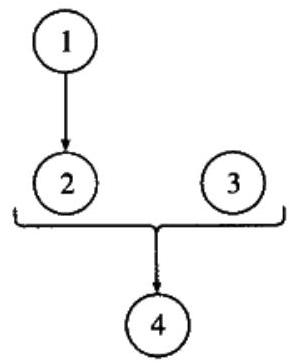
\includegraphics[max width=\textwidth, center]{2025_05_15_6a28331d5e7c993ad07ag-050}

2.义务投票最大的优越性在于,通过促使投票人走向投票站,使大家平等地参与投票,消除人们对少数特权公民的偏见。还有另外两个重大的优越性:一是义务投票可以减少金钱在政治中的作用,因为它使候选人和政治党派无须花费大量金钱去促使投票人走向投票站。二是它降低了对负面宣传的刺激。\\
--Arend Lijphart,"Compulsory Voting Is the Best Way to Keep Democracy Strong",The Chronicle of Higher Edu- cation, 18 October 1996

3.生命不单是我们所拥有的一个"好"事。我们的生命便是我们的自我。将我们的生命作为可以允许他人去终止的"事情",这是极其非人性的。安乐死,即便是有法定能力的人所请求的安乐死,也是对人类特性和局限性的挑战。\\
--Ramsey Colloquium of the Institute on Religion and Public Life,"Always to Care,Never to Kill",Wall Street Jour- nal, 27 November 1991\\
4.体育运动对高等教育的所有积极贡献受到一些坏风气的威胁,特别是一些重要的运动项目所受威胁更大。这些坏风气植根于制度上的冷漠,校长的忽视,以及与不择手段地取胜相关联的不断增长的体育商业化趋势等。不幸的事实是,校园内主要以赢利为目的的体育运

动已经失控。\\
-Keeping Faith with the Student-Athlete: A New Model for Intercollegiate Athletics, Knight Foundation Commission on Intercolle- giate Athletics,Charlotte,NC,March 1991\\
*5.著名经济学家 J.K.加尔布雷斯长期致力于揭示并改善一个社会现实,即"个人富有而社会贫穷"。在其经典著作《富裕的社会》(1960)中,他论证如下:

人们愿意购买真空吸尘器以保证房子的清洁,在我们的生活水平上这也是必需的。而清洁街道的吸尘器却被当做不必要的花费。其结果,我们的房子一般是清洁的,而我们的街道通常是不干净的。\\
——Cited by John Cassidy,"Height of Elo- quence",The New Yorker, 30 November 1998

6.让我们追溯到1884年,民主党候选人格里弗•克利夫兰面临着他是一个私生子的父亲的指控。那时共和党人唱道:"妈,妈,我爸在哪儿?"克利夫兰承认了他供养着那个孩子,没有遁词,也没有回避。他的一个支持者对投票人提出了下列忠告:

既然格里弗•克利夫兰有一个良好的公众记录,但有一个有污点的私生活,既然他的对手詹姆士•G•布莱茵有一个如小说中描绘的完美的私生活,但有一个颇多波折的公众记录,为什么不把他们两人放在各自表现得最好的位置上呢——让布菜茵回到私生活中去,让克利夫兰保持公众生活。

7.由于力量总是在被统治者一边,统治者用于支持自身的除了與论之外别无他物。因此政府只是建立在舆论之上的。\\
--David Hume,cited in Keith Thomas,"Just Say Yes",The New York Review of Books,

8.认识功能依赖于大脑中受酶影响的神经化学作用。这些酶由基因构成。如果智力功能没有受基因的影响,那将是令人惊奇的。\\
——Gerald E.McClearn,"Genes a Lifelong Fac- tor in Intelligence",New York Times, 6 June 1997

9.当代礼仪标准进一步证实我们的判断,这样一个年轻人(15 岁)是没有为重罪行为负责的能力的。缺乏经验、缺少教育以及缺乏理解力,使得十几岁的青少年不能正确评价其行为的后果,同时他们与成年人相比更易于感情用事或更易于受同伴压力的影响。

不能期望对青少年处以死刑可以阻止 16 岁以下的青少年犯谋杀罪,因为让十几岁的肇事者去做成本一收益分析,去掂量被处以死刑的可能,这是根本不现实的。\\
-Justice John Paul Stevens,Thompson v.Oklahoma, 487 U.S.815, 1988\\
*10."最好的人"和"最好的黑人"之间的两分法不是由种族主义者制造出来用以诋毁非白人专业人员的能力的东西。相反,这种两分法不时得到一些大学生的强化,这些学生要求学校雇用一定数量的少数族裔雇员 $\cdots \cdots$ 他们(实际上)是说"去雇最好的黑人"。这种两分法进一步得到了全体教员的支持,他们认为学生的这些要求不过仅仅是对公正的诉求。\\
--Stephen L.Carter,"The Best Black,and Other Tales",Reconstruction,vol.1, Winter 1990

11.过去存在吗?不存在。将来存在吗?不存在。那么只有现在存在。是的。但是在现在之中就没有时间的流逝吗?当然有。那么时间不存在吗?哦,我希望你不要如此讨厌。\\
-Bertrand Russell,Human Knowledge, 1948\\
12.给小费不能提高服务质量;如果能提高,出租车司机将比航空服务员更有礼貌。而且,给小费是有损尊严的,因为它模糊了酬金与馈赠之间的界限,把出钱人和服务者都放在了一个易受伤害的位置上。\\
-_George Jochnowitz,"Let's Dispense with Tipping Altogether",New York Times,

13.如果没有灰尘就没有曙光,没有蔚蓝的天空,没有美丽的日落,天空中也没有任何一种颜色能吸引风景画家的目光。如果光线不是被空气中无数细微的灰尘微粒消散,太阳光的热量将使人无法忍受。如果没有灰尘作为集结场所,雨云就不能很容易地形成,那样白天将非常炎热而夜晚将十分寒冷。概而言之,灰尘使地球上的生命成为可能。\\
-Ivor Smullen,"Homage to a Speck", The Sciences,April 1992\\
14.以前的中间等级的下层,即小工业家、小商人和小食利者,手工业者和农民——所有这些阶级都降落到无产阶级的队伍里来了,有的是因为他们的小资本不足以经营大工业,经不起较大的资本家的竞争;有的是因为他们的手艺已经被新的生产方法弄得不值钱了。无产阶级就是这样从居民的所有阶级中得到补充的。\\
-Karl Marx and Friedrich Engels,The Communist Manifesto, 1848\\
*15.因为我立刻感到喜欢诺兰•米尔斯,在他的回答中我听到的是坚强和自信。如果不是由于我已感到喜欢他,那么在他的回答中我听到的就会是傲慢与恐吓。第一印象成了自我实现的预言:我们听到的是我们希望听到的东西。这场访谈毫无办法地带有充满好感的偏见。\\
-Malcom Gladwell,"The New-Boy Net- work",The New Yorker, 29 May 2000\\
16.没有人能够完全词达其意,也很少有人能够词尽其意,因为词语是溜滑的,而思想是黏滞的。\\
-Henry Adams,The Education of Henry Adams(1907),chapter 31\\
17.自然选择感兴趣的是行为而不是大脑中所思考的东西。这意味着给人们提供真信念的自然选择的机会是很少的,因此人们有足够的理由去怀疑仅仅由自然选择产生的固守在头脑中的信念。\\
--Prof.Alvin Plantinga,quoted in"Science and Sensibility",Insight, 18 August 1997\\
18.削减学费会减少学校从政府资助项目中获取的收人,政府的资助在特定情况下是基于收费总额的,因此在降低学费问题上有一个内在的制约因素。\\
--David Spadafora,"Don't Expect Many Colleges to Lower Tuition",New York Times, 1 January 1996\\
19.最有效的税制改革是:降低资本利润税率。不要将主要财力和精力用于寻找对资本利润征税的办法,而将更多的精力用于企业投资。应把出于低成本考虑而套在已到期的投资上的资本解放出来,用于新的风险投资。这样政府税收和新的投资都会上升,有益于投资者、政府和企业家等所有各方。\\
-Bruce C.Lueck,"Cut the Capital Gains Tax",New York Times, 2 December 1996\\
*20.土著美国人关于过去和死亡的信念确实值得尊重,但是不应用这些信念支配政府政策去调查和解释早期美国史前史的方略。如果必须在人类起源的对抗理论之间做出选择的话,应当首先选择基于科学方法的理论。只有科学的理论才是建立在经验证据之上的,只有科学的理论才有可能被修正和推翻。\\
-R.Bonnichsen and A.L.Schneider,"Bat- tle of the Bones",The Sciences,August 2000

\subsection{1. 6 论证和说明}
许多语段,无论是书面语还是口语,看起来好像是论证,实际上不是论证而是说明。即使有某些前提或结论指示词出现,例如"因为"、"由于"、"因此"等,也不能解决问题,因为这些语词既可用在论证中也可用在说明中。我们必须知道在这些语段中作者的意图。[41]

请比较下面两段话:

1.为你自己积损财宝在天上,天上没有虫子咬,不能锈坏,也没有淢挖窟窟来偷,因为你的财宝在哪里,你的心也在哪里。

2.所以它(那座塔)名叫巴别,因为耶和华在那里变乱天下人的言语。\\
——《创世记》11: 19

第一段话是一个清楚的论证,它的结论,即一个人必须积攒财宝在天上,由前提(这里用"因为"来标明)一个人的财宝积攒在哪里,他的心也在哪里来支持。但是第二段不是论证,尽管它非常恰当地使用了"所以"一词。它说明了这座塔(其建造过程在《创世记》中有详细的叙述)为什么叫巴别。它告诉我们,因为之前人类在那里使用的是同一种语言,现在被许多语言变乱了,所以给塔起了这个名字。 ${ }^{[42]}$ 这段话假设读者知道那座塔有这个名字,意图是说明为什么给塔起了这个名字。短语"所以它名叫巴别"不是结论而是完成了对这个名字的说明。句子"因为耶和华在那里变乱天下人的言语"不是前提,它不能作为相信巴别是那座塔名字的原因,因为巴别是那座塔的名字的事实是这段话所要为之做说明的读者所知道的。在这个语境中"因为"指示的是接下来要说明将巴别这个名字给予那座塔的原因。

上面两段话说明一个事实,表面上相似的语段可能具有完全不同的功能。任何一个特定的语段究竟是论证还是说明,这取决于那个语段所服务的目的。如果我们的目的是要确立某个命题 Q 的真,为此我们提出某个证据 P 来支持 Q ,我们可以恰当地说" Q 因为 P "。也就是说我们为 Q 建立一个论证, P 是我们的前提。但是假设 Q 是已知为真的。在这种情况下我们不必提出任何理由来支持它的真一一但是我们可以希望对它为什么是真的给出一个说明。这样我们也可以说" Q 因为 P "——但在这种情况下,我们不是为 Q 建立一个论证,而是给出一个对 Q 的说明。

在回答关于类星体(在我们的星系以外很远地方的一类天体)的外观颜色的问题时,一位科学家写道:

\begin{displayquote}
最远的类星体看上去像强烈的红外辐射光点。这是因为太空散布着吸收蓝光的氢微粒 (大约每立方米两个微粒), 如果你从可见的白光里过滤掉蓝光, 那么剩下的就是红光。在其到达地球的数十䎲光年的旅程中, 类星体光被大气中的氢微粒吸去了全部的蓝光, 留下的只有红光。[43]
\end{displayquote}

这段话不是论证,它不是试图要让读者确信类星体具有像它们所显示的外观颜色,而是说明它们具有这个外观颜色的原因。

同样,在讨论不列颠对非洲早期发展的影响时,一个历史学家写道:

\begin{abstract}
塞拉利昂在1808年成为英国直辖殖民地不是因为它的繁荣,而是因为它的萧条。由于战争和商业不景气的负担,塞拉利昂的私营公司不能支付它们的费用,而刚刚废除了贩卖奴隶制度的英国政府感到有必要接管它。 ${ }^{[44]}$
\end{abstract}

这里没有对塞拉利昂在1808年成为英国直辖殖民地这个结论进行论证。塞拉利昂在那时确实成了英国直辖殖民地。但这是为什么呢?乃是由于在本例和前例中,"因为"很明显是说明的标志,而不是论证的标志。

我们怎么才能断定一个语段的目的是打算说明还是打算说服人呢?通常我们可以根据" Q 因为 P "这个形式提问,对于作者来说 Q 的身份是什么,以此来做出区分。若 Q 是一个其真实性需要建立的命题,那么"因为 P "可能给出了支持其为真的前提,这样"Q 因为 P "就是一个论证。若 Q 是一个已知其为真,或至少在这个语境中其真是没有疑问的命题,那么"因为 P "就可能是对为什么 Q 成为真命题的阐释,这样" Q 因为 P "就是一个说明。

在一个说明中,人们必须把什么是被说明的东西,与什么是用来说明的东西区别开来。在上面《创世记》所做出的说明中,被说明的内容是为何那座塔具有名字巴别,说明的内容是在那里耶和华变乱天下人的言语。在上面刚给出的历史学的例子中,被说明的内容是塞拉利昂成为不列颠直辖殖民地,说明的内容是塞拉利昂公司的无支付能力和不列颠政府就此做出的回应。

有时被称做说明的东西实际上可能是论证,反之亦然。不久以前,《纽约时报》由于对待男女性别的不平等做法而受到一个读者的批评,因为它对一个著名女演员的不断增长的体重加以评论,但对在同一篇报道中提到的一个杰出商人的不断增长的体重却没有评论。后有另一个读者对此做出回应:

E.R.福克斯的抱怨——你特别提到凯瑟琳•丹尼芙"也许不像她以前那么苗条",但你没有提及唐纳德•杜鲁普不断增加

的腰围——很容易说明。杜鲁普先生从未裸体出现在电影中以使他的体形成为人们感兴趣的事情。 ${ }^{[45]}$

这不是一个真正的说明,而是一个论证。它有两个前提,第一,裸体外表出现在电影中使一个人的外表成为人们感兴趣的事情,第二,杜鲁普先生从未以裸体外表出现在电影中,而丹尼芙女士有过。因此,报纸对如此出现在电影中的名人的体形加以评论,而忽略未如此出现在电影中的名人的体形,这种做法就是合乎情理的(这个读者的主张),据此抱怨对待男女性别不平等就是不应当的。

为了区别说明和论证,我们必须对语境有一定的敏感性。总会有一些语段,其目的难以确定。一个其目的难以确定的语段可能需要给予两种同样有道理的"解读"一一用一种方法去解读,被当做论证;用另一种方法解读,就是说明。

\subsection{练习题}
下列各段话有些包含说明,有些包含论证,有些既可作为论证也可作为说明。你对每段话的主要功能的判断是什么?断定其作为论证或说明的理由是什么?如果是论证,请指出其前提和结论;如果是说明,请指出被说明者和说明者。

\subsection{例题}
1.统一税率的想法为什么会吸引人,这个问题并不神秘。现行的税收制度复杂得令人恼火,而且执行起来代价昂贵。它奖赏消费惩罚储蓄,与经济学的通常观念正相反。在许多情况下它显然是不公平的——例如许多有工作的夫妇为他们的共同收人所支付的税款,要远远高于那些住在一起却分别报税的未婚夫妻所支付的税款。\\
——David E.Rosenbaum,"Panel Calls for a Flat Tax",New York Times, 18 January 1996

\subsection{解答}
这段话表面上是对统一税率为什么吸引人的一个说明:它吸引人是因为现行的税收制度存在着不足,并指出了其中的几点不足。但这段话也可看做是支持统一税率的一个论证,现行税收制度的几点不足是前提,结论\\
(未明确表述)是现行税收制度应当被统一税率取代。\\
哪个解释更接近于作者意图取决于这段话的语境。如果语境是对两种可供选择的税收制度作一个没有偏见的公正比较的话,这段话可能主要是一个说明。但是因为这段话出现在对一个提倡统一税率的一个专门组织的报道中,我们可以得出结论,它实际上主要是一个支持统一税率的论证。

2.在今天的医学研究中不使用动物将是不道德的和自私的。如果使用动物的研究被终止,将会对我们的后代造成更大的伤害。\\
-_Science,Medicine,and Animals(Wash- ington,DC:National Academy of Sci- ence,Institute of Medicine,1991)

3.生来便无再繁殖特性的动物已经灭绝,而繁殖能力强的动物将它们的基因遗传给了后代。粗略地说,因为较强的性功能是长期进化而来的,那些性欲强的动物比性欲弱的动物能产下更多的后代。\\
-R.Thornhill and C.T.Palmer,"Why Men Rape",The Sciences,February 2000

4.变化是真实的。既然变化仅在时间上是可能的,那么时间一定是某种真实的东西。\\
-Immanuel Kant,Critique of Pure Reason (1781),"Transcendental Aesthetic", section II\\
*5.黑洞是一个有着什么也不能逃脱它的巨大引力的物体——即使宇宙中最快的光也不能逃脱它。任何向黑洞靠近的东西都会被吸进这个物体而消失,就像是掉进了洞穴之中。因为连光都不能从其中逃逸出来,这个洞看起来是漆黑的。\\
-Ken Croswell,"The Best Black Hole in the Galaxy",Astronomy,March 1992

6.列举事态的原因不是为事态辩解。事情因其结果而不是因其先行条件被证明是正当的或是应受谴责的。\\
-_John Dewey,"The Liberal College and Its Enemies",The Independent, 1924

7.因为他是我儿子,因为我爱他胜过对世界上任何事物的爱,胜过我能想象的对任何人的爱,甚至胜过我对他母亲的爱,我在他身旁爬行,

我的躯干钻进了壁橱,而我的腿还钩在地毯上。\\
--Michael G.Jaffe,Dance Real Slow (New York:Farrar,Straus and Giroux, 1996)

8.我喜欢瓦格纳的音乐胜过任何人的音乐。它的乐声如此响亮,以至于即使有人一直在说话,人们也不会听见他在说什么。\\
-Oscar Wilde,The Picture of Dorian Gray, 1891

9.从赫伯特•胡佛到杰米•卡特,每一位总统都将他们的总统档案捐赠给公众。只有尼克松提出诉讼要求为他的档案付费。多年来,尼克松的律师以隐私权为由反对任何公众接触尼克松的录音带。现在(1999 年)仍要求为那些录音带及其他材料付费的做法是荒谬的,因为尼克松可能早已利用迫使他下台的那些证据而获利。\\
-"A Curious Claim by the Nixon Estate", New York Times, 22 February 1999\\
* 10 .爱情是不用眼睛而用心灵看着的,因此生着翅膀的丘比特常被描画成盲目。\\
-William Shakespeare,A Midsummer Night's Dream,act 1,scene 1

11.与别的哺乳动物相比,灵长目动物有一个特别长的幼儿依赖期,因为据信,他们需要时间去学习其独特的复杂社会的各种规则。\\
——Meredith F.Small,"Political Animal", The Sciences,March 1990

12.受理诉讼主要是书面艺术,这有两个后果:第一,不读案情摘要,经常很难弄清楚最高法院辩论的内容;第二,最高法院的任何一个诉讼决议可能与口头辩论时所涉及的问题无甚关联,而是反映案情摘要中的内容。对最高法院的辩论进行电视转播可能只是使人对法院如何工作产生误解,而不是使得诉讼过程非神秘化。\\
-Andrew C.Mergen,"Where Words Are Worth 1000 Pictures",New York Times, 8 May 1996

13.刺客总是比疾病更容易使美国总统丧命或致残,因此对于总统的

健康和安全,联邦特工比总统的医生有更多的事要做。\\
--George J.Annas,"The Health of the President and Presidential Candidates", New England Journal of Medicine, 5 October 1995\\
14.人们经常认为炎症只是一个讨厌的症状。但是炎症不只是标志着伤害,它还能使伤害永久存在——以恶性循环的形式。这就是为什么像关节炎那样的轻病会使人致残,并且是慢性的、难以治愈的。这也是为什么病人愿意冒很大的风险去使用能带来暂时缓解同时也会带来一些严重后果的药品。\\
-Jerome Groopman,"Superaspirin",The New Yorker, 15 June 1998\\
*15.在科学课上女孩子怎么会变得害怕提问题呢?她们怎么会比男孩子更觉得科学无用或无趣呢?她们的这种态度是学来的,她们的父母和老师教会了她们这样。\\
-"Why Are There Fewer Women?"Mich- igan Alumnus,October 1995\\
16.不断增长的监禁率没有导致犯罪率的降低,因为终归没有多少罪犯被关押或逮捕。这不是因为法官对犯人太软弱,而是因为百分之九十的罪行没有被告发,或者案件悬而未决。\\
-Elizabeth Alexander,"Look to More Cost-effective Antidotes than Prison", New York Times, 25 January 1996\\
17.一个人可能受别人制定的法律管束,但是不可能在任何一个自己可以自由行使意愿的问题上束缚自己。……因此国王必然不可能受自己制定的法律支配。由于这个原因,我们可以用一句惯用语来评价王室的法令和条例:"因为我们很高兴这样做(for such is our good pleasure)"。\\
--Jean Bodin,Six Books of the Common- wealth, 1576\\
18.资产阶级的反抗,由于资产阶级被推翻(哪怕是在一个国家内)而凶猛十倍;资产阶级的强大不仅在于国际资本的力量,在于它的各种国际联系牢固有力,而且还在于习惯的力量,小生产的力量。这是因为世界

上可惜还有很多很多小生产,而小生产是经常地、每日每时地、自发地和大批地产生着资本主义和资产阶级的。由于这一切原因,无产阶级专政是必要的,不进行长期的、顽强的、拼命的、殊死的战争,不进行需要坚持 41 不解、纪律严明、坚定不移、百折不挠和意志统一的战争,便不能战胜资产阶级。\\
—V.I.Lenin,"Left Wing"Communism: An Infantile Disorder, 1920\\
19.联邦通讯委员会和纽约州公共服务委员会,都没有接到多少对电话号码簿不准确的投诉。这是因为在看账单时,人们没有意识到他们要为一句"空号"的错误应答付费。而不管是否提供了最新号码信息,电话号码簿的制作者照样可以拿到报酬,他们没有任何动力改进其服务。\\
--Bradley F.Taylor,"No Listing?Dial M for'Maddening'",New York Times, 29 August 2000\\
*20.按照任何标准,美国人的科学教育都很成问题。很多被当做科学来教的东西往往并不必要。在小学,学生经常被灌输反科学和恐惧数学的思想。在中学和大部分高校,许多科学内容经常被略去。因而对大部分美国大学生而言,对科学素养的要求简直就是一个悲哀的笑话。\\
-Leon M.Lederman,"Science Education, Science,and American Culture",The Key Reporter,Winter 1992\\
21.所有动物种群的规模每年都变化不定,这取决于自然条件的优 (和暖的天气,丰富的食物)与劣(旱灾,严冬,饥荒)。当条件恶劣时,小种群更可能濒临灭绝,因为小种群的规模本来就小。小种群也更容易受到各种形式的人类残害和自然灾祸的致命一击。所以,小种群比大种群面临更大的危险。孤岛上的种群——包括那些被圈养在生态孤岛上的种群,比如被发达的社区包围的公园——正日益变小。\\
-David Quammen,"National Parks:Nature's Dead End",New York Times, 28 July 1996

22.因为物体的引力随物体质量的增大而增大,物体越重其引力就越大。离物体越近,其引力越强。所以有些物体的体积很小但引力很大。这

就是为什么白矮星一一大约是太阳那么大的质量装到地球那么大的体积里的恒星——会产生如此强大的引力。\\
--Marcia Bartusiak,"To the Edge of Space", Astronomy,July 1998\\
23.乔治-梅森是我的一个祖先,他极力主张在宪法公约中废除奴隶制,称它"对人类是不光彩的"。这个尝试失败以后,他强烈要求国会将他的"权利宣言"作为权利法案通过。这也被拒绝了。所以他拒绝签署这个宪法。\\
--Thomas C.Southerland,Jr.,"A Virginia Model",New York Times, 5 July 1997\\
24.母鼠生男生女的比例依生活状况的变化而改变。当母鼠生活闲适,又与健壮的公鼠结成配偶时,就生出过量的儿子;当世道艰难,或最近丢失了幼鼠时,就生出更多的女儿。

养活女儿似乎比较"廉价",母亲花很少的时间去啝抚和喂养她们,在断奶时她们比儿子个头小很多。她们的性别也更安全,几乎肯定会生儿育女,把其母亲的基因传下去。相反,儿子的性别被认为是赌注性的,理论上在母亲把他们养育到性成熟以后他们会很优秀,他们能比他们的姐妹生育更多的后代。因此当母亲们有精力和资源养育子女时,她们就有一个进化的正当理由去生育更多娇贵的儿子;当前景悲观时,她们就自动选择生育能抗御恶劣生存条件的女儿。母亲们不知如何从她们的栖息地吸取了有关的信息,并把这些信息转化成出生比例的改变。\\
-_"How Biology Affects Behavior and Vice Versa",New York Times, 30 May 1995\\
*25.我们——无论黑人还是白人,富人还是穷人,男性还是女性,保守人士还是自由人士——视而不见关在监狱里的 700000 名黑人(1994年),而在1960年只有 25000 人;视而不见因杀戮而死的 11000 人 (1993 年)(数字来源于司法统计局);视而不见失业及与其他社群相比远远落后的期望寿命。这个美国阶层没有思想库,没有政治团体,没有政治说客。作家拉夫•魏莱认为,这就是黑人孩子倾向于枪击的原因。\\
-Bill Stephney,"Rap Star's Death High- lights Harsher Reality",New York Times, 18 September 1996

\section*{1.7 演绎和有效性}
每一个论证都是断言其前提为结论的真提供理由。实际上这种断言正是论证的标志。但是论证有两大不同种类:演绎论证和归纳论证。这两类论证在其前提支持结论的方式上有着根本的不同。本节我们对演绎论证作一个简要的阐释。

任一演绎论证均断言其前提决定性地(conclusively)支持结论。相反,归纳论证均没有这种断言。在对一个语段的解释中,如果我们判定它做出了 43 这样的断言,我们就将其视为演绎论证;如果我们判定它没有做出这样的断言,我们就将其视为归纳论证。因为每个论证都会对决定性支持结论或者做出断言,或者不做出断定,所以每个论证或者是演绎的,或者是归纳的。

当一个论证断言它的前提(如果是真的)为它的结论的真提供了无可辩驳的理由时,这个断言或者是正确的或者是不正确的。如果是正确的,这个论证就是有效的。如果不是正确的(也就是说,即使前提是真的,也不能无可辩驳地确立其结论的真),那么这个论证就是无效的。

因此,对于逻辑学家而言,有效性这个术语仅仅对演绎论证才是适当的。说一个演绎论证是有效的,就是说如果其前提是真的,其结论为假就是不可能的。这样我们可把"有效性"定义如下:一个演绎论证是有效的,即如果其前提是真的,则其结论必定是真的。

每个演绎论证都要求其前提为其结论的真提供担保,但并非所有演绎论证都能做到这个要求。不能做到这个要求的演绎论证就是无效的。

因为每个演绎论证就其目标的实现而言或者是成功的或者是不成功的,所以每个演绎论证或者是有效的或者是无效的。这一点非常重要:如果一个演绎论证不是有效的,它一定是无效的;如果它不是无效的,它一定是有效的。

演绎逻辑的中心任务(将在本书第二部分详细讨论)就是对有效论证和无效论证做出区分。为此,古往今来逻辑学家们发明了许多非常有效的方法。但用来判定论证有效性的传统方法不同于大多数现代逻辑学家使用的方法。前者被叫做古典逻辑,发端于亚里士多德的分析工作,本书的第5、6、7章将对此加以阐释。现代符号逻辑的方法将在本书的第8、9、 10 章详加介绍。尽管两个流派的逻辑学家们在方法上和对某些论证的

具体阐释上不尽一致,但他们都同意演绎逻辑的主要任务是开发一种能使我们区分有效论证与无效论证的工具。

\section*{1.8 归纳和或然性}
归纳论证不要求它们的前提必然地支持结论,纵然其前提是真的。它提出一个较弱的但仍然是很重要的要求:其前提或然性地支持结论。或然性总是必然性的缺乏,因而上述关于有效性和无效性的讨论并不适用于归纳论证:归纳论证既不是有效的也不是无效的。 ${ }^{[46]}$ 当然,我们仍然可以对它们进行评估。实际上,对归纳论证进行评估是任何领域的科学家最主要的任务之一。归纳论证的前提为它的结论提供某种支持,前提授予结论的或然性程度越高,论证的价值也就越大。一般情况下,我们可以说归纳论证"较好"或"较差","较弱"或"较强",等等。但是,甚至在所有前提都是真的并且对其结论提供了非常强的支持的情况下,归纳论证的结论也不是必然得出的。归纳理论,归纳推理的技巧,评估归纳论证的方法,以及量化和推测或然概率的方法等将在本书第三部分详加介绍。

归纳论证和演绎论证之间的区别是根本性的。因为归纳论证的前提对其结论的支持都具有某种程度的或然性,附加的信息就有可能强化或弱化这种或然性。新发现的事实可以使我们改变对或然性的估价,可能导致我们对归纳论证的判定比我们原想的更好(或更差)。在归纳论证的领域——即使当结论被认为具有很高可能性的情况下——永远不会穷尽所有的证据。正是这种发现与我们以前所相信的证据相冲突的新材料的可能性,使得我们不能断定任何归纳论证的结论具有绝对的确定性。

相反,演绎论证却不能越来越好或越来越差。它们在显示前提和结论之间的令人信服的关系上要么成功要么失败。这个对比揭示了演绎和归纳之间的根本差异。如果一个演绎论证是有效的,就没有附加的前提可以增强这个论证的有效性。例如,如果凡人皆终有一死,并且如果苏格拉底是人,我们就可以毫无保留地得出结论,苏格拉底终有一死——即苏格拉底终有一死的结论总能从那两个前提推论出来,而不管世界上别的什么可能是真的,也不管别的什么信息被发现或增加到该论证的前提当中。比如我们后来又知道苏格拉底难看,或天使永生,或奶牛产奶,但这些发现和别的发现都不能对原来的论证产生任何影响。

就每一个有效的演绎论证来说,不管附加前提的性质如何,从其前提必然推出的结论同样也能必然地从任何扩大的前提集推论出来。如果一个论证是有效的,世界上就没有什么东西能使它更有效;如果一个结论是从某个前提集有效推出的,就没有什么东西可以增加到这个前提集当中使得该结论的推出变得更严格、更合乎逻辑或更有效。

但归纳论证并不是这样,归纳论证所断言的前提和结论之间的关系远非如此严格,与演绎论证有本质上的不同。考虑下面这个归纳论证:

\begin{displayquote}
大部分公司法律顾问是保守主义者,\\
安吉拉•帕尔默瑞是一个公司法律顾问,所以安吉拉•帕尔默瑞很可能是保守主义者。
\end{displayquote}

45 这是一个非常好的归纳论证,它的第一个前提是真的,如果它的第二个前提也是真的,则其结论很可能就是真的而不是假的。但是在这种场合(与有关苏格拉底的必死性的论证形成鲜明对照),若增加某个新前提到原来的论证之中,就可能会弱化或强化(依据新前提的内容)原来的论证。假设我们还知道:

\section*{安吉拉•帕尔默瑞是美国公民自由权协会(ACLU)的一名官员。}
又假设在原论证中增加一个(真)前提:

美国公民自由权协会的大部分官员不是保守主义者。

那么那个结论(安吉拉•帕尔默瑞是一个保守主义者)不再看起来非常可能,原来的归纳论证由于这个关于安吉拉•帕尔默瑞的附加信息的出现而被大大弱化。而如果上述前提被改造成全称命题:

没有美国公民自由权协会的官员是保守主义者。

那么就会有效地从被断定的前提集演绎地推出与原来结论相反的结论。

另一方面,假设我们通过增加下面的附加前提来扩大原来的前提集:

安吉拉•帕尔默瑞长期是国家步枪协会(NRA)的一名宫员。

和\\
安吉拉•帕尔默瑞被任命为保守的《国家评论》报的特约撰稿人。

那么通过这个扩大了的前提集,原来的结论就得到了比原来的前提集更大的支持。

总之,归纳和演绎的区别依赖于两类论证对前提和结论之间的关系所作断言的性质。我们可以将两类论证的特征表示如下:

演绎论证是一种其结论被断言为从其前提绝对必然地推出的论证,这种必然性不是一个程度问题,不以任何其他事物情况为转移。反之,归纳论证是一种其结论被断言为仅仅或然性地从其前提推出的论证,这种或然性是一个程度问题,其程度受可能出现的其他事物情况的影响。

归纳论证并不总是明确表明其结论仅仅是在某种或然程度上推出来的。另一方面,在一个论证中出现"或然性"一词也并不一定表明该论证就是归纳的。这是因为有一些严格的演绎论证是关于或然性本身的。 ${ }^{[47]}$ 在这种论证中,事件之间的确定联系的或然性是从另外的事件的或然性演绎推出的,这个问题将在第 14 章讨论。

\section*{1.9 有效性和真实性}
如前表明,一个成功的演绎论证是有效的。有效性指谓命题之间的一种关联一一作为演绎论证前提的命题集和作为该论证的结论的一个命题之间的关联。如果后者是逻辑必然地从前者推出的,我们就说该论证是有效的。因为归纳论证永远达不到逻辑必然,有效性永远不适用它们。有效性也永远不能适用于任何独立的单一命题本身,因为在任何一个命题内部都不可能找到这种必需的关联。

另一方面,真和假都是单个命题的特征。在论证中作为前提的单个陈述可能是真的或假的,作为其结论的陈述可能是真的或假的。结论可以被

有效地推论出来,但是说任何结论或任何单一的前提本身是有效的或无效的,都是无意义的。

真,是其断言与实际情形相一致的命题的属性。当我断定苏必利尔湖是北美洲五大湖中最大的湖时,我的断言确与实际情形相一致,从而就是真的。如果我说北美洲五大湖中最大的是密歇根湖,我的断定就与实在世界不一致,因此就是假的。这个对比是重要的:真和假是单一的命题或陈述的属性;有效性和无效性是论证的属性。

正如有效性这个概念不适用于单一的命题,真这个概念也不能应用于论证。一个论证中的几个命题,其中的一些(或全部)可以是真的,并且其中的一些(或全部)可以是假的。但是论证作为一个整体,既不"真"也不"假"。关于世界的陈述的命题可以是真的或假的,由从一个命题集到其他命题的推论构成的演绎论证可以是有效的或无效的。

真(或假)命题与有效(或无效)论证之间的关系处于演绎逻辑的中心地位。本书第二部分主要致力于分析它们之间的这些复杂关系。不过,在这里对有效性和真实性之间的关系作一初步的讨论也是适宜的。

即使一个论证的一个或几个前提不是真的,这个论证也可能是有效的,我们的讨论就从强调这一点人手。每个论证都对其前提和从这些前提推导出的结论之间的关联做出断言;即使这些前提被证明为假或其真实性受到质疑,这种关联也是成立的。1858年亚伯拉罕•林肯在与斯蒂芬•道格拉斯的一场争论中有力地运用了这一点。林肯对强迫逃跑到北方各州的奴隶返回他们在南方的主人家里的德雷德-司各特决议进行抨击说:

考虑到人们的论辩能力,我把德雷德•司各特决议用三段论形式表述如下,可以看出这个论证中是否有错误:

任何一个州的任何法规和法律都不能破坏美国宪法中所清楚、明确地规定的权利。

美国宪法中清楚、明确地规定了对奴隶的财产权。\\
所以任何一个州的任何法规和法律都不能破坏对奴隶的财产权。

我相信这个论证挑不出什么毛病。假设其前提都是真的,从这些前提必然会推出上述结论,这个结论我完全有能力理解。但我认为其中确有一个毛病,但这毛病不在于推理,事实上这个毛

病是有一个前提是错误的。我相信对奴隶的财产权并不是宪法中清楚明确地规定的,而道格拉斯法官认为是的。我相信最高法院和那个决议(德雷德•司各特决议)的拥护者要想在宪法中查找到对奴隶的财产权的清楚明确的规定将会是徒劳的。所以我说,我认为事实上上述推理前提之一不是真的。 ${ }^{[48]}$

在他加以概括并予以抨击的那个论证中,林肯发现第二个前提——美国宪法中规定了对奴隶的财产权——明显是假的。他指出,那个论证中的推理不是错误的,然而它的结论却没有得到证明。林肯的逻辑观点是正确的:甚至在一个论证的结论和其一个或几个前提都为假时,这个论证也可以是有效的。我们再一次强调,一个论证的有效性仅仅依赖于其前提与结论之间的关联。

在有效的和无效的论证中,真的和假的前提与结论之间有许多可能的组合。考虑下列作为例示的论证,每一个论证之前都有一个对其前提与结论的真假组合的简短陈述。通过这些例证,我们可以完整地列出有关真实性和有效性之间的关系的重要原则。

I.有些有效的论证只包含真命题——真前提和真结论。

所有哺乳动物都有肺,所有鲸鱼都是哺乳动物,所以所有鲸鱼都有肺。

II.有些有效的论证只包含假命题:

所有四条腿的生物都有翅膀,所有蜘蛛都是四条腿的,所以所有蜘蛛都有翅膀。

这个论证是有效的,因为如果其前提是真的,其结论也一定是真的一一即 48使我们知道这个论证的前提和结论实际上都是假的。

III.有些无效的论证只包含真命题一一它们的所有前提都是真的,它

们的结论也是真的。

如果我拥有福特•诺克斯的所有财富,那么我将是富有的,我不拥有福特•诺克斯的所有财富,所以我不是富有的。

N.一些无效的论证只包含真前提,但有一个假结论。这可以用一个与前面的论证(III)在形式上完全相同,仅仅换一个假结论的论证来说明:

如果比尔•盖茨拥有福特•诺克斯的所有财富,那么比尔•盖茨将是富有的,

比尔•盖茨不拥有福特•诺克斯的所有财富,\\
所以比尔•盖茨不是富有的。

这个论证的前提是真的,但结论是假的。这样的论证不会是有效的,因为有效的论证不可能前提真而结论假。

V.有些有效的论证有假前提和真结论:

所有鱼是哺乳动物,\\
所有鲸是鱼,\\
所以所有鲸是哺乳动物。

如我们所知,这个论证的结论是真的;而这个结论可以从两个都不符合实际的假前提有效地推论出来。

V.一些无效的论证也有假前提和真结论:

所有哺乳动物都有翅膀,\\
所有鲸都有翅膀,\\
所以所有鲸都是哺乳动物。

从例 V 和例 VI 可以看出,很显然我们不能从一个论证有假前提和真结

VI.当然,有些无效的论证包含的都是假命题——假前提和假结论:

所有哺乳动物都有翅膀,\\
所有鲸都有翅膀,\\
所以所有哺乳动物都是鲸。

这七个例子清楚地表明,有结论为假的有效论证(例II),也有结论为真的无效论证(例III和例IV)。因此很显然,一个论证的结论的真或假自身并不决定那个论证的有效性或无效性。此外,一个论证有效不能保证其结论的真实性(例 II)。

下面两个表格(涉及前面的七个例子)清楚地表明了论证前提与结论可能组合的种类。第一个表格表明,无效论证可以具有真的和假的前提与结论的每一种可能组合:

第二个表格表明,有效论证只能具有真的和假的前提与结论的可能组合的三种情况:

第二个表格的那个空格位置显示了非常重要的一点:如果一个论证是有效的并且其前提都是真的,我们就可以断定其结论也是真的。换句话说:如果一个论证是有效的并且其结论是假的,那么其前提不会都是真的。有些完全有效的论证确有假结论一一但是任一这样的论证必定至少有一个假前提。

若一个论证有效,并且其所有前提都为真,我们就称它为"可靠的" (sound)论证。很显然,一个可靠论证的结论一定是真的一一并且只有可\\
论这个事实分辨出这个论证究竟是有效的还是无效的。\\
VI.当然,有些无效的论证包含的都是假命题——假前提和假结论:\\
所有哺乳动物都有翅膀,\\
膀,\\
所以所有形动数。\\
这\\
$\qquad$论的真实性(例 II)。可能组合的种类。第一个表格表明,无效论证可以具有真的和假的前提与\\
结论的每一种可能组合。

\begin{center}
\begin{tabular}{|c|c|c|}
\hline
\multicolumn{3}{|c|}{无效的论证} \\
\hline
真结论 & 假结论 &  \\
\hline
真前提 & 例 III & 例 IV \\
\hline
假前提 & 例 VI & 例 VI \\
\hline
\end{tabular}
\end{center}

第二个表格表明,有效论证只能具有真的和假的前提与结论的可能组合的三种情况:

\begin{center}
\begin{tabular}{|c|c|c|}
\hline
\multicolumn{3}{|c|}{有效的论证} \\
\hline
\multicolumn{3}{|c|}{真结论} \\
\hline
真前提 & 例 I & 假结论 \\
\hline
假前提 & 例 V & 例 II \\
\hline
\end{tabular}
\end{center}

第二个表格的那个空格位置显示了非常重要的一点:如果一个论证是有效的并且其前提都是真的,我们就可以断定其结论也是真的。换句话\\
说: 如果一个论证是有效的并且其结论是假的, 那么其前提不会都是真一个假前提。靠论证才能确立其结论的真实性。如果一个演绎论证不是可靠的——也就

是说,如果这个论证不是有效的,或者如果其前提并非都是真的一一即使其结论事实上是真的,其结论的真实性在论证中也得不到确立。

检验前提的真实性或虚假性是一般科学的任务,因为前提完全可以涉及任意的题材。逻辑学家的主要兴趣不在于命题的真实性或虚假性,而在于命题之间的逻辑关系。所谓命题之间的"逻辑"关系,指的是决定其所出现于其中的论证的(形式)正确性或不正确性的命题之间的那些关系。决定论证的(形式)正确性或不正确性的任务正好落在逻辑学的领域内。逻辑学家甚至对前提可能为假的论证的(形式)正确性感兴趣。

为什么不把我们的研究限制在真前提论证的范围内,而忽略所有其他论证呢?这是因为,那些前提的真实性不为人们所知的论证的(形式)正确性,有可能是非常重要的。例如,在科学研究中,我们通过推断出可检验的结果来检验理论——但是我们不能预先知道哪个理论是真的。又如,在日常生活中,我们经常必须在可供选择的两个行动方向之间做出选择,推断每个行动方向的后果。为了避免选错,我们必须对可供选择的两个选项做出正确的推理,将每个选择作为一个前提。如果我们仅仅对前提为真的论证感兴趣,那么只有当我们知道了可供选择的两个前提哪个是真的,我们才能知道去找出它的结论集。但是如果我们知道可供选择的两个前提哪个是真的,我们就完全不必对它做出推理,因为我们推理的目的就是帮助我们对应该断定哪一个可供选择的前提为真做出决定。所以,如果把我们的注意力限制在前提已知为真的论证上,将使我们的目标不能实现。

确定演绎论证的有效性或无效性的一些富有成效的方法将在本书第二部分介绍并阐释。

\section*{1. 10 复杂的论证性语段}
实际论证有可能是非常复杂的。有些语段中的论证是由几个论证多重复合而成,语段中有些命题只作为前提,有些命题既作为前提又作为分结论,这样的语段分析起来就比较困难。图示法的技术就非常有助于分析这种语段,但并不存在一种建构图示以精确地描述这样的语段的机械方法。此外,因为对这种语段可以作几种合理的解释,因此也可以合理地考虑几种不同图示来展现其逻辑结构。

为了清楚地分析复杂语段,我们必须努力理解作者推理的流程,辨识

语段中每个成分的作用。下面的例子(为便于分析,其中的分支命题用数字标出)显示了我们阐明前提和结论之间的联系的方法。一旦辨识出一段话语中所含的论证以及论证之间的关系,我们就能够对这些论证的结论是否真正是从被断定的前提中推论出来的做出判定。

在下列论证集合中,语段最后的结论就是第一个陈述,这不奇怪。有四个前提直接支持这个结论,其中的两个前提又是分结论,逐次得到语段中所断言的其他前提不同方式的支持:

\begin{displayquote}
(1)看来, 用动物实验进行科学研究的做法并不是不必要的或靠不住的; (2)在使用脊椎动物进行实验之前, 实验的草案必须经过包括一名兽医和一名公众代表在内的公共机构委员会进行的再审查, 并且(3)在研究期间, 动物的医疗和卫生情况得到定期监测。(4)研究者需要健康的动物进行科学研究和医学研究, 因为(5)不健康的动物可能导致错误的研究结果。这激励(6)科学家确保他们使用的任何动物健康并且营养良好。此外, (7)用动物进行研究是昂贵的, 因为(8)料学研究的资金受到限制, (9)只有高质量的研究才能通过有力的竞争获得对研究的支持。[49]
\end{displayquote}

下面的图示展示了这段话的逻辑结构。检查这样的图示,从那些在图中最高处因而在逻辑串联中也是最早的地方开始,通过用数字替换表达出来的命题,有助于对它们进行"解读"。也就是说,人们能够从推理的几条路线的每一条路径推出最后的结论。\\
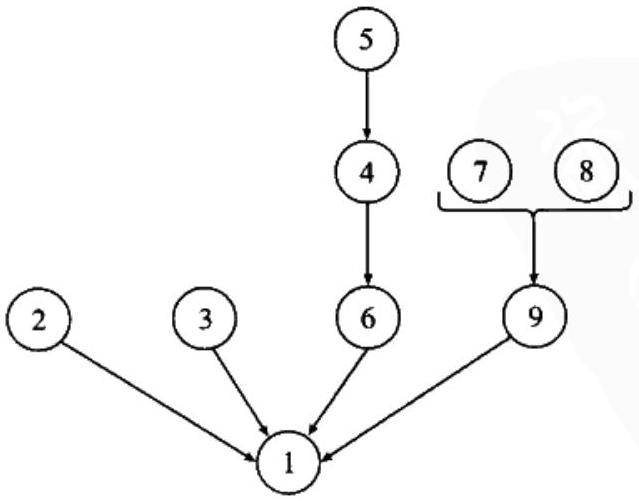
\includegraphics[max width=\textwidth, center]{2025_05_15_6a28331d5e7c993ad07ag-072}

在一个论证中,单个的命题有时以不同语词表达的语句形式重复出现,有时是为了强调,有时又被省略。这种强调使得分析工作复杂化。图示法有助于分析,因为我们可以用相同的数字表示相同命题的不同表述。下面一段话由三个清楚的论证构成,有些命题重复多次出现:

\begin{displayquote}
(1)宇宙大爆炸理论正在瓦解……(2)根据正统知识, 宇宙起源于大爆炸一 -200 亿年前的一次巨大的、非常匀称的爆炸。问题是(3)天文学家通过进一步观测证实: 现存的巨大星系团因为体积太大, 完全不可能在仅仅 200 亿年时间中形成……通过人造卫星所收集的新材料的研究, 以及较早前的地面测量表明(4)星系聚集成绵延数十亿光年的巨大带状, 并且(5)星系之间有亿方光年的距离。因为(6)据观测, 星系移动的速度远不及光速, 数学家证明(7)聚集成这么大的物质团必须要经过至少 1000 亿年时间一是假设的大爆炸时间的五倍……(3)像那么大的一种结构现在看来不可能在 200亿年时间中形成……(2)大爆炸理论认为, 物质均匀地散布在宇宙中。而与这种理想理论相反, (3)这么巨大的星丛无法这么快地形成。[50]
\end{displayquote}

在这段话中,报告观察证据的前提(4)、(5)、(6)为(7)即自大爆炸起必须经过非常长的时间提供理由。这被用来支持分结论(以三种略有不同的方式表述)即(3)像那么大的一种结构现在看来因为太大,不可能在那段时间中形成。从 (3)这个结论,结合(2)即对大爆炸理论假设的原始对称和扩散的简短陈述(以两种略有不同的方式表述),我们可以推论出这段话最后的结论(1):大爆炸理论正在瓦解——这段话开头的命题。下面的图示展示了这段话的逻辑关系集:\\
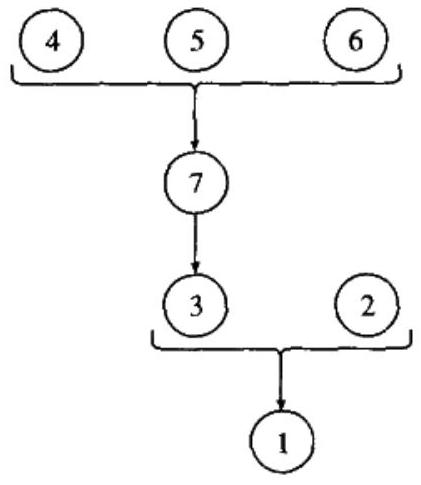
\includegraphics[max width=\textwidth, center]{2025_05_15_6a28331d5e7c993ad07ag-073}

分析论证,必须注意前提可能以浓缩形式出现的情形,有时前提只以一个名词性短语来表示。在下面的论证中短语"在大气中的散射"作为前提(4),可以重塑为"太阳的能量散射在大气中"。浓缩与重复使得对下列论证的分析更加困难:

\begin{displayquote}
(1)太阳能汽车只是一种试验性的装置, 其他什么都不是。(2)太阳的能量太弱以至于不能发动甚至是日常使用的迷你汽车。(3)进入大气层的太阳能量大约为每平方码 1 千瓦。因为(4)在大气中的散射, 又因为(5)地球上的任何地方一天中平均只有半天时间受到阳光的照射, (6)每天接收的太阳功率平均为 $1 / 6$ 千瓦时到 4千瓦时 $\cdots \cdots$ 对通常规格的汽车的检测表明, (7)若使一辆电车勉强能够工作, 其电池组需要 300 千瓦时的能量。因此, (8)充满汽车电池必须有 40 平方码的原电池, 大约是一辆拖拉机的拖车顶部的尺寸。(1)除了用于昂贵的试验汽车外, 太阳能没有指望成为任何汽车的动力, 太阳能汽车不是一项待开发的技术。这就是结论。[51]
\end{displayquote}

这段话中的第一个命题,即"太阳能汽车只是一种试验性的装置,其他什么都不是"的断定,是最后的结论。语段的最后以更加复杂的形式重复了这一结论。这段话的图示为:\\
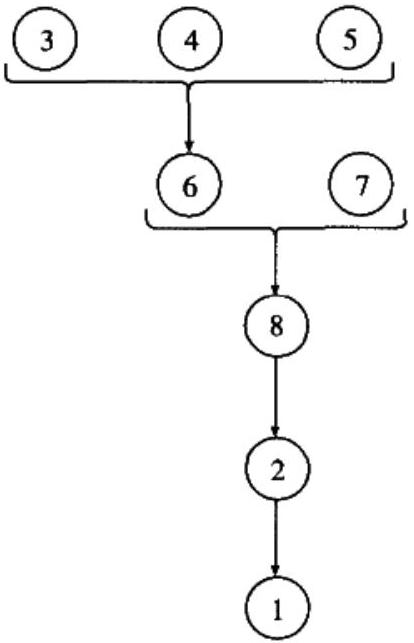
\includegraphics[max width=\textwidth, center]{2025_05_15_6a28331d5e7c993ad07ag-074}

在我们分析复杂的论证性话语时,即使是一些包含许多前提和分结论的语段,我们也经常发现它们是非常融贯的、清楚的。请看一位女编辑为其引起争论的编辑方针进行辩护时所写的一段话:

本刊(《新英格兰医学杂志》)的主张是(1)不发表不道德的研究报告,忽略它们的料学价值……

我们的主张有三个理由。首先,(2)如果普遍坚持这个主张,只发表合乎道德的研究文章,将会阻止不合乎道德的研究工作的开展。(3)文章的发表是医学研究奖赏制度的一个重要部分。(4)如果研究者知道他们不合乎道德的研究成果不能发表,他们就不会去做不道德的研究。(5)而相反的做法将有助于导致更多的不道德研究工作的开展,因为,如我已表明的,(6)这样的研究可能比较容易开展,因而(7)可能使从事不道德研究工作的人处于有利的竞争地位。其次,(8)即使发表不道德的研究成果不妨碍发表合乎道德的研究成果,为了坚持把合乎道德放在研究第一位的原则,也应该拒绝不道德的研究。(9)如果允许有所松动,我们将逐渐变得习惯于发表不道德的研究成果,并且(10)这将导致对发表合乎道德的研究成果的极大妨碍。最后,(11)对不道德研究成果的拒绝,有利于使社会普遍注意到,甚至某些科学家也不懂得科学研究应是文明的基本尺度。(12)知识尽管很重要,但对一个公平公正的社会来说知识或许远不及得到知识的方法重要。 ${ }^{[52]}$

最后的结论也出现在语段开头,(2)、(8)和(11)三个主要命题直接支持这个结论,这三个前提本身又得到处于不同位置的其他几个前提的支持。语段中的众多命题,在导出结论的过程中都有一个清楚的逻辑作用,共同服务于整个语段要证明的结论:不合乎道德的研究报告将不能在《新英格兰医学杂志》上发表,它们的科学价值也应被忽略。下页的图示展示了这个虽然复杂但推理缜密的语段的逻辑结构。

日常生活中的论证经常达不到这样的水准。它们可能包含着作用不清楚的陈述;论证中陈述与陈述之间的连接可能相互纠缠或被错述;甚至在论证者的头脑中论证的流程可能本来就是混乱的。由图示支持的逻辑分析\\
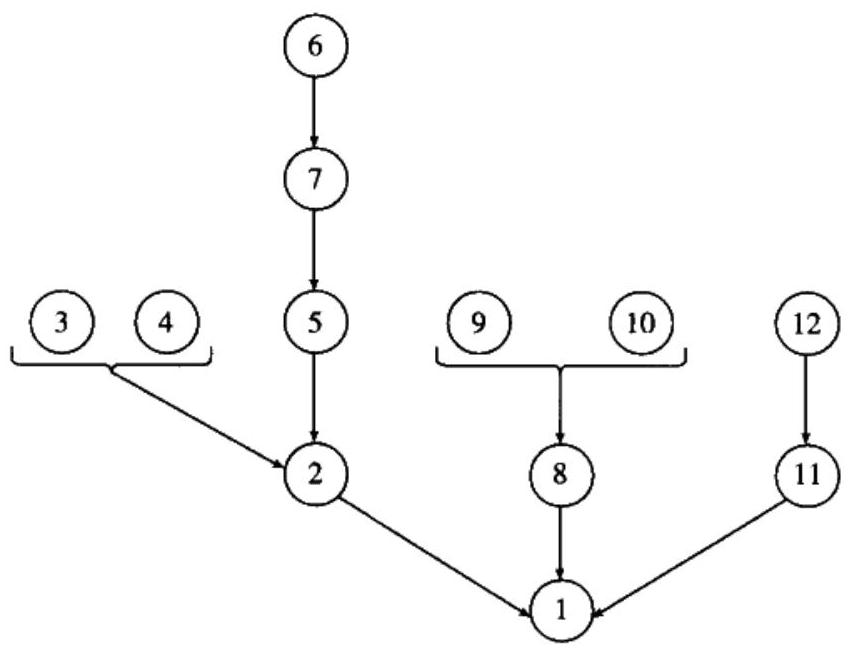
\includegraphics[max width=\textwidth, center]{2025_05_15_6a28331d5e7c993ad07ag-076}

可以暴露这些不足。通过使一个推理过程的结构暴露出来,我们能看到推理过程是如何展开的,推理的长处与缺陷是什么。逻辑学的一个特殊领域就是对实际论证的评估,成功的评估需要对所分析的论证有一个清楚的把握。

\section*{练习题}
下列每段话都包含几个论证,其前提和结论的排列方式不尽相同。分析这些语段,必要时解析其前提和结论,并为每段话构建一个图示。\\
*1.民主政体的法律一般保护最大多数人的利益,因为它们源于大多数的公民,这些公民易于犯错,但他们不会站在自己利益的反面。相反,寡头政治的法律有助于将财富和权力集中在少数人手中,因为从本质上看,寡头政治是由少数人建构起来的。因此可以断定,一般情况下,民主政体的立法宗旨比寡头政治的立法宗旨对人类更有益。\\
——Alexis de Tocqueville,Democracy in A- merica, 1835

2.父亲和母亲的基因可能是互相对抗的。让我们来考虑怀孕问题。就大部分哺乳动物而言,母亲的身体将不断长大的胚胎当做人侵者,努力限制胚胎对其体内营养的摄取。当然,父亲不生产后代,不必考虑这类问题,但其基因的遗传学的重要性是无疑的:促进胚胎发育,保护胚胎使其

发育不受母亲身体自我保护的影响。因此,只有男性的基因才促进像胎盘那样已知的胚胎保护器官的生长,而女性的基因不能。单亲的鼠类卵细胞,来自单一的母亲基因,发育成正常的胚胎,但这个胚胎没有胎盘,因此比较脆弱。\\
--Laurence Marschall,in a review of $\mathrm{Ge}^{-}$ nome,by Matt Ridley(HarperCollins, 2000),appearing in The Sciences,Au- gust 2000\\
3.有一个问题:(对君王来说)是受人爱戴比被人畏惧更好呢,还是被人畏惧比受人爱戴更好?应当希望二者兼而有之,但是,将二者结合在一个人身上是困难的。若二者不可兼得,被人敬畏比受人爱戴要安全得多。因为可以断定,一般人是忘恩负义的、易变的、虚伪的、胆怯的、贪婪的……若信赖他们的诺言而缺乏其他准备,这样的君王是很危险的。因为尽管君王可以通过金钱买来友谊,但是这样的友谊是没有保障的,在需要的时刻是不能依靠的。人们对于冒犯一个爱戴的人比冒犯一个畏惧的人更少顾忌,因为爱戴是以恩义这条纽带维系的,而由于人的劣根性,这条纽带常常由于利益缘故而被斩断。但是对你的畏惧则基于对惩罚的恐惧而不会消失。\\
——N.Machiavelli,The Prince, 1515\\
4.想一想为什么联邦政府会参与向学生贷款?这是因为从国家利益考虑,需要有一个接受过教育的大众群体。大学毕业生平均比高中毕业生年薪要高两倍。国家在贷款学生的教育上投资,可以在提高生产力和增加国家收人方面得到高出好多倍的回报。通过解决数百万美国人的教育问题,联邦政府资助的贷款学生为美国国库创造了巨大的回馈,因为随着学位的提高,他们的收人及应交的税款,就大大地提高了。

但多数大学生都不具备良好的贷款信度。典型的学生形象是:没什么现钱和可做抵押的资产,平时赚钱太少,以致贷款信度不高。如果这样的借款者能够得到一笔(通常的)贷款的话,那么往往其利息也会很高,以致高得让许多学生做出不上大学的决定。这就是为什么学生贷款需由联邦资金支持,而且所收利息也有上限规定的原因。\\
--Richard W.Riley,"Should Washington Have a Bigger Share of the Student-loan\\
*5."...…咱们初次会面时,我就对你说过,你是从阿富汗来的,你当时好像还很惊讶哩。"\\
"没问题,一定有人告诉过你。"\\
"根本没有那回事。我当时一看就知道你是从阿富汗来的。由于长久以来的习惯,一系列的思索飞也似的掠过我的脑际,因此在我得出结论时,竟未觉察得出结论所经的步骤。但这中间是有着一定的步骤的。在你这件事上,我的推理过程是这样的:‘这一位先生,具有医务工作者的风度,但却是一副军人气概。那么,显见他是个军医。他刚从热带回来,因为他脸色黝黑,但那并不是他原来的肤色,因为他的手腕的皮肤是白皙的。他久病初愈而又历尽艰辛,因为他面容憔悴。他左臂受过伤,现在动作看来还有些僵硬不便。试问,一个英国的军医在热带地方历尽艰苦,并且臂部负过伤,这能在什么地方呢?自然只有在阿富汗了。这一连串的思想,历时不到一秒钟,因此我便脱口说出你是从阿富汗来的,你当时还感到惊讶哩。"

我微笑着说:"听你这样一解释,这件事还是相当简单的呢。"\\
--A.Conan Doyle,A Study in Scarlet, 1887

6.与量子研究相关的最困难的问题之一是,如何在使其不受影响的自然状态下去观察原子内部的粒子——也就是非破坏性地观察它们。这个困难有两个原因。第一,原子和原子内部的粒子是构成物质的最小部分。因为观察它们的工具都放射出其自身的能量,这个能量一定会影响被观察粒子的能量。第二,在孤立情况下,原子的组成部分同时以两种量子状态存在着一一粒子和波。它们好像是统计概率组成的包。只有在它们与其他组成部分相互作用时,它们才显现出这种或那种表现形式。\\
——Skinning Schrodinger's Cat,Insight, 15 July 1996\\
7.科学为神秘事物留下任何空间了吗?米切尔•J•贝赫在《达尔文的黑盒子》(Darwin's Black Box,The Free Press,1996)中坚决主张肯定回答。他证明说,作为生命基础的细胞内部作用的起源不能用自然选择或任何别的纯粹基于机会的途径来解释。用现代生物学的强大工具进行考察,生物化学水平上的生命(在这位专业生物化学家看来)只能是神明设计的产品。

他的论证的关键是,细胞内部的基本秩序是"不可化约地复杂的";它们由几个特有的相互作用的部分组成,每个组成部分在作为一个整体的系统功能上均起着关键作用。例如,去掉导致血液凝结反应的复杂过程的任何一步,一个受伤生物体的生命所必需的血液就会像水从一个破杯子里流出那样泄漏出去;但是要将一个阻止凝血过程的单个的酶迁移到受伤的部位,全部的血液供应就会变硬起来。因为这两种情况都将是致命的,血凝块分子的组成部分不能通过自然选择逐渐地聚集到一起从而集合成一个作用系统。

8.美国邮政局没有一个明确的机制来处理疑难问题或推动机构改革。没有公民可以拥有可交易的股份。经理和工作人员的收人和安全由邮政局对第一类邮件的垄断、公共基金和雇员对国会的政治影响来保证。公众不能将邮政局的业务转交给更有能力的竞争者,因为竞争是被禁止的。因此,美国邮政的严重低效率不是由邮政雇员自身的原因造成的,而是邮政局自身的结构造成的。\\
--Douglas K.Adie,"Privatizing Will Im- prove Mail Service Posthaste",Insight, 30 January 1995\\
9.取消对婚姻征税听起来像一个好主意。但是对富人征收高比率税,以及对不管配偶双方的收人是合计的还是分计的家庭征收同样税赋的想法,也是合理的。没有任何税法能同时实现这三个目标。其个人收人分别只够被征百分之十五的税的两个人,按照累进税制,当他们的收人被合计时,他们就可进人被征税百分之二十八的除层。国会可以取消婚姻税,但只能通过牺牲累进税制的方法。\\
-"Temptations of a Balanced Budget",Ed- itorial in New York Times, 31 December 1997\\
*10.没有东西是可解证的,除非其反面意指一个矛盾。没有东西可以清楚地可想象地意指一个矛盾。无论我们设想为存在物的是什么,我们也可以设想其为不存在物。因此,没有其不存在性意指一个矛盾的存在物。因而,没有一个其存在性是可解证的存在物。\\
-David Hume,Dialogues Concerning

\subsection*{1.11 推 理}
如前所述,逻辑学是研究用于区分正确推理与不正确推理的方法和原理的学问。推理与论证都是从已知的(或为了某种目的而肯定的)前提推出结论的过程。至此,我们一直在分析和评估的是别人的论证。当然,我们在决定自己应如何行动、评价他人的行动、为道德的或政治的信念进行辩护等方面,我们每天都要建构我们自己的论证。建构和运用好的论证之技能是有巨大价值的。

推理的技能可以通过训练来提高。为了促进这样的训练,许多推理游戏(例如国际象棋、围棋、Mastermind ${ }^{(1)}$ 等)都是极好的手段。而那些用以强化和测试我们的逻辑技能的推理谜题,也无疑是相当实用的。推理不仅是一项必要的活动,也是一项愉快的活动——当我们解决了为提高技能和使人娱乐双重目的而设计的一些逻辑问题时,它所产生的乐趣是不言而喻的。

人为设计的问题比现实生活中的问题更简洁,通常也更简单。但是解答它们是具有挑战性的,经常需要锲而不舍地反复推理,这在思考模式上与侦探或新闻工作者或陪审员没有很大不同。可能需要找到一个推理系列,在这个系列中,所得的次结论被用做后来推理的前提。也可能要求具有一定的洞察能力,要找到解决问题的路径需要对早先假设或发现的信息进行创造性的重组。解决人为设计的问题往往是比较困难的,有时会无功而返,但是当通过推理的成功应用解决了问题时,是非常令人满足的。逻辑游戏和谜题解答,伴随各种推理模型的运用,都是很好的娱乐。"对思虑的享受",美国哲学家约翰•杜威写道,"是受过训练的大脑的标志"。

推理问题的一个常见类型是智力测验,仅仅使用所提供的线索,我们被要求理清和辨识有关的几个人物的名宁,或角色,或其他事实。下面是一个比较简单的例子:

在某个航班的全体乘务员中,飞机驾驶员、副驾驶员和飞行工程师的职务由爱伦、布朗和卡尔三人担任,但不必是这个

\footnotetext{(1)种著名的网络智力游戏。
}次序。\\
副驾驶员是个独生子,钱挣得最少。\\
卡尔与布朗的姐姐结了婚,钱挣得比驾驶员多。\\
问:三个人每人担任什么职务?

为了解答这样的问题,我们首先要寻找一个范围,在这个范围中我们 59 有足够的信息去得到超出前提所给信息的一些结论。我们从前提中知道许多关于卡尔的情况:他不是飞机驾驶员,因为他挣得比驾驶员多;他也不是副桇驶员,因为副驾驶员挣得最少。通过排除我们可以推出,卡尔一定是飞行工程师。

使用上述的次结论,我们可以确定布朗的职务。布朗不是副驾驶员,因为他有一个姐姐而副驾驶员是个独生子;他也不是飞行工程师,因为卡尔是飞行工程师。所以布朗一定是飞机驾驶员,而仅剩的爱伦一定是副驾驶员。

在解答这类问题(有时非常复杂)时,建构一个备选项的图示是非常有帮助的,这种图示叫做矩阵,当我们积累了新的信息时就把它填人表中。要见识这种矩阵图的作用,请考虑下面的问题:

阿伦佐、库特、鲁道夫和威拉德是四个天资极高的创造性的艺术家。一个是舞蹈家,一个是画家,一个是歌唱家,一个是作家,但不必是这个次序。\\
(1)那天晚上歌唱家在音乐会舞台上进行他的首次演出时,阿伦佐和鲁道夫在观众席上。\\
(2)库特和作家两人有画家为他们画的生活肖像。\\
(3)作家正准备写一本阿伦佐的传记,他写的威拉德的传记是畅销书。\\
(4)阿伦佐从未听说过鲁道夫。\\
问:每个人的艺术领域是什么?

将这些前提中断定的许多事实记在头脑中,也记住几个可以从这些前提推出的分结论,这是一项必需的工作。把我们的推论记在便条上可能是有帮助的,但是也可能导致混淆和零乱。我们需要一种有效方法,来贮备

已知的信息和所引出来的中间结论,能把已知的信息和推出的信息整齐地记录下来,并随着推论的数目不断增长以及论证的链条不断拉长供我们使用。而在我们要建构的矩阵表中就有空间去表示所有相关的可能选择,并能记录下每一个引出的推论。

这个问题的矩阵表必须是显示这四个人(用四行表示)和他们从事的四种艺术职业(用四列表示)的一个列阵,如下所示:

\begin{center}
\begin{tabular}{|l|l|l|l|l|}
\hline
 & 舞蹈家 & 画家 & 歌唱家 & 作家 \\
\hline
阿伦佐 &  &  &  &  \\
\hline
库 特 &  &  &  &  \\
\hline
鲁道夫 &  &  &  &  \\
\hline
威拉徳 &  &  &  &  \\
\hline
\end{tabular}
\end{center}

当我们断定名字在某行左边的人不可能是从事某列顶端所示职业的艺术家时,我们就在那个人名字的右边以那个职业做标题的列中空格写一个 N (代表"no",或写一个"一"符)。我们立即可以从前提(1)做出推断,阿伦佐和鲁道夫都不是歌唱家,所以我们在第三列(歌唱家)他们名字的右边空格写上一个 N。同样,我们可以从前提(2)推断库特既非画家也非作家,所以我们把一个 N 记在第二列(画家)和第四列(作家)他的名字右边的空格中。从前提(3)我们看出作家既非阿伦佐也非威拉德,所以我们把 $N$ 记在第四列他们名字右边的空格中。至此我们记录的所有项目都得到了原先所给信息的证明,现在的矩阵表如下:

\begin{center}
\begin{tabular}{|l|l|l|l|l|}
\hline
 & 舞蹈家 & 画家 & 歌唱家 & 作家 \\
\hline
阿伦佐 &  &  & N & N \\
\hline
库 特 &  & N &  & N \\
\hline
鲁道夫 &  &  & N &  \\
\hline
威拉德 &  &  &  & N \\
\hline
\end{tabular}
\end{center}

从已获得的信息我们可以用排除法断定,鲁道夫一定是作家,所以我们在第四列(作家)下鲁道夫名字右边的空格中记一个 Y(代表"yes",或记一个"+"符)。现在从列阵看,很明显,画家一定或是阿伦佐或是威拉德,并且我们在这里可以排除阿伦佐:鲁道夫有画家给他画的肖像(从前提(2)可知),阿伦佐从未听说过鲁道夫(从前提(4)可知),因此阿伦

佐不可能是画家。这样我们记一个 N 在第二列(画家)阿伦佐名字右边的空格中。

接着我们可断定阿伦佐一定是舞蹈家,从而在第一列(舞蹈家)阿伦佐名字右边的空格记一个 Y。现在我们可以在舞蹈家列中为库特和威拉德二人分别记人一个 N 。对库特来说剩下的唯一可能是歌唱家,所以我们记一个 Y 在那个空格中,并且记一个 N 在威拉德名字右边歌唱家列的空格中。再通过排除我们断定,威拉德一定是画家,并将一个 Y 填入矩阵表的最后一个空格。完成的图示是这样的:

\begin{center}
\begin{tabular}{|c|c|c|c|c|}
\hline
 & 舞蹈家 & 画家 & 歌唱家 & 作家 \\
\hline
阿伦佐 & Y & N & N & N \\
\hline
库 特 & N & N & Y & N \\
\hline
鲁道夫 & N & N & N & Y \\
\hline
威拉德 & N & Y & N & N \\
\hline
\end{tabular}
\end{center}

从这个填满的矩阵表中我们可以得到答案:阿伦佐是舞蹈家,库特是歌唱家,鲁道夫是作家,威拉德是画家。

当要求提供几种不同范围的答案时,这种综合性质的智力游戏就变得更复杂了。有些这样的问题非常具有挑战性,并且不使用矩阵方法几乎不可能解决。 ${ }^{[53]}$

另一些推理问题提出的是一种不同的挑战。下面是一个精致、娱人但不是很困难的问题。在阅读紧随其后的答案之前请努力解决它。

你面前有六个球:两个红球、两个绿球和两个蓝球。在每一对同色球中,你知道其中一个比另一个重。你还知道所有三个重球的重量相同,所有三个轻球也一样重。另外,这六个球(把它们分别叫做 R1、R2、G1、 G2、B1 和 B2)难以区分。你只有一架天平秤盘。

问:若在秤盘上称量不能超过两次,如何能辨认出所有三对球中的重球和轻球?

\section*{答案:第一次称量: $\mathbf{R 1 + G 1 / / R 2 + B 1}$}
如果两边平衡:R1 和 R2一对红球中,一个重一个轻。因两个红球分别在秤盘的两边,我们知道如果两边平衡,那么每一边的另一个球一定也是一重一轻——因为如果两个重球在同一边,这一边就一定沉下去。因此,我们知道两者必居其一:G1 重而 B1 轻,或者 G1 轻而 B1 重。

如果在第一次称量时两边平衡,那么第二次称量:G1//B1。无论这一次称量的结果是什么,所有球的轻重都可以辨认出来。

如果(在这次称量中)G1 沉下去,那么:\\
-G1 重(且 G2 轻),且\\
-B 1 轻(且 B 2 重),且\\
$\cdots \mathrm{R} 1$ 轻(且 R2 重)。\\
如果(在这次称量中)G1 升上去:(上述结论的)反面就是真的。\\
但是,倘使在第一次称量中 $(\mathrm{R} 1+\mathrm{G} 1 / / \mathrm{R} 2+\mathrm{B} 1)$ 两边不平衡将会怎样?假设 $\mathrm{R} 1+\mathrm{G} 1$ 沉下去。(如果 $\mathrm{R} 1+\mathrm{G} 1$ 升上去,随之答案就简单地倒转过来。)

我们知道在这种情况下 R1(在这一边的红球沉下去)一定是重的;因为如果 R1 是轻的,R2 就是重的;并且如果 R2 是重的,R1+G1 就不会沉下去。

因为 R1 是重的,下面三种联合体之一一定是如此这般:\\
(a)G1 是轻的,并且 B 1 是轻的;或者\\
(b)G1 是重的,并且 B 1 是重的;或者\\
(c)G1 是重的,并且 B1 是轻的。

\section*{如果 $\mathbf{R 1 + G 1 ~}$ 在第一次称量中沉下去,第二次称量: $\mathbf{R 1 + R 2 / /}$ $\mathrm{G} 1+\mathrm{B} 1$ 。}
我们已经知道 R1 是重的。在这第二次称量中,R1+R2(重 + 轻)一定是下列两种情况之一:沉下去或升上去,或者两边平衡。无论是哪一种结果,我们都可以辨认出所有球的轻重如下:\\
(x)如果 R1+R2 沉下去,G1 和 B1 一定都是轻的(因为一个重的加一个轻的会在重量上超过仅仅两个轻的相加)。在这种情况下联合体一定是上面的(a)型:G1 是轻的且 B1 是轻的一一所有问题都被解决。\\
(y)如果 R1+R2 升上去,G1 和 B1 一定都是重的(因为重+轻在重量上只能被两个重的相加超过)。在这种情况下联合体一定是上面的(b)型:G1 是重的且 B1 是重的——所有问题都被解决。\\
(z)如果两边平衡,G1 和 B1 也一定是重+轻。在这种情况下联合体一定是上面的(c)型:G1 是重的且 B1 是轻的一一所有问题都被解决。

将这个问题推荐给你的朋友们之前,请练习说明上述答案!\\
在现实世界中,我们经常被要求从某个当前事态推出它的起因,从事

情现在是什么推出其过去是什么。科学家——特别是考古学家、地质学家、天文学家、医学家——通常面对着探究其起源的事件或条件。企图说明事情为何从过去的状况发展到现在的状况的推理叫做回溯分析。例如,令天文学家惊奇的是,1996年在地球旁边疾驰而过的彗星海库塔克(Hy- akutake)放射出比任何一位科学家曾预言的一颗彗星能够放射出的强 100倍的可变 X 射线。德国马克斯-普朗克研究所的一位彗星专家评论说: "为了研究这些数据,我们中断了我们正在进行的工作——但这是一种你喜欢拥有的问题。"

我们确实喜欢拥有这样的问题。因此,回溯分析问题经常是为娱乐而设计的。然而这样的问题也有一种特殊的困难:由科学的或历史的知识提供的现实世界的逻辑框架一定是以某种方式由问题自身规定的。一些规则或规律一定是在逻辑分析能够进行的范围内提出的。

棋盘是一种最著名的回溯分析问题的装置,而下棋规则规定了必要的 63 理论语境。下棋无须什么技术,但对(国际)象棋规则不熟悉的读者可以跳过如下例示。

象棋中的回溯问题通常采取这样的形式:棋盘中棋子的安排是给定的,对一局棋赛进行回溯分析,以比赛中遵守了所有比赛规则为前提。例如,图 1-1 代表一局棋赛所得到的形势,比赛中所有的着数都与象棋规则一致。那么,刚刚走的一着棋或几着棋是什么?\\
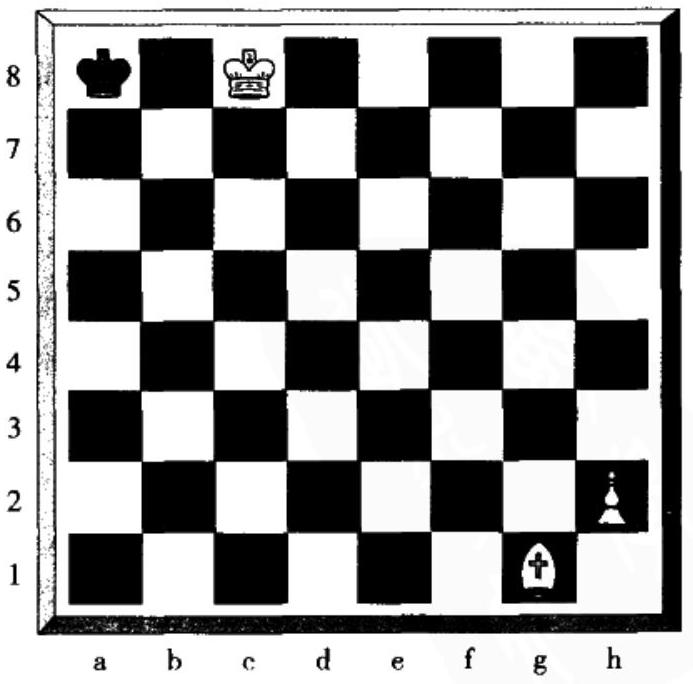
\includegraphics[max width=\textwidth, center]{2025_05_15_6a28331d5e7c993ad07ag-085}

图 1-1

为便于分析,所有行数从下到上加标数字 1 到 8 ,所有列数从左到右加标字母 a 到 h。那么棋盘中每一个方格都能用一个唯一的字母一数字结合体表示:黑王在 $a 8$ ,白兵在 $h 2$ ,等等。问题是:上一步由黑棋走的那着棋是什么?那么黑棋的前一步白棋的着数是什么?你能在阅读下一段之前推出答案吗?

答案:刚走的一着棋是黑王移动。因为两个王永远不能走在邻近的方格里,黑王不可能刚从 b7 或 b8 走到现在的位置上;因此我们可以确定黑王刚从 a 7 走到现在的位置,在 a 7 处黑王被将军。

这是非常容易推断的。但是前一着白棋是什么才能使黑王处于被将军的局面呢?那着棋不可能是白象(在 g1),因为白象没有一条路径能走到 g 1 格,不可能在白象走棋时黑王正处于被将军的局面!因此一定是,黑王被将军的局面是由另一个白棋子的移动造成的,这个白棋子正阻挡着象的攻击,并被走到 $a 8$ 的黑王吃掉。什么白棋子能在黑对角线上并且从那儿走到角上的白格中呢?只有在 $b 6$ 的马。所以我们可以确定,在黑棋最后一着(黑王从 a 7 到 a 8 )之前,白棋最后一着是从 $b 6$ 到 a 8 的马。 ${ }^{[54]}$

当然,现实生活中我们所面对的推理问题很少像本节所讨论的谜题这样整洁。许多现实问题的叙述不是很精确的,对它们的错误描述易于使人误解,从而不能得到答案。遇到这种情况,原问题的部分陈述就要加以拒绝或替换。而当我们试图解答本章给出的这种逻辑谜题时,我们是不能这么做的。

此外,现实世界中的一些问题,甚至当它们被准确描述时,也可能是不完善的,其中某个最初不是可供利用的条件,可能对于问题的解决是必不可少的。现实世界中一些问题的答案可能依赖于某个新的科学发现,或某个以前不可想象的发明或装置,或对某个至今未加探索的领域的研究。但是在逻辑谜题的陈述中,如同一部好的谋杀案侦探小说一样,必须给出足以得到答案的全部信息;否则我们就会认为侦探小说作家,或问题的设计者对我们是不公平的。

最后,逻辑谜题提出的问题都是清楚明确的(诸如:四个艺术家中哪一位是歌唱家?黑棋和白棋的最后一着是什么?等等),给出其答案并加以证明,就明确解决了逻辑谜题提出的问题。但那不是许多现实世界中的问题所呈现的形式。现实问题最初经常是仅仅由于某种前后矛盾的情形或一个不平常的事件的出现而被发现的,甚或只是基于人们对某种事情之不

顺畅的感觉而发现的——现实问题不是有着明确答案的精心构造的问题。\\
不管有多少区别,现实世界中的问题与精心设计的逻辑问题一样,都必须通过系统的推理才能得到解决,二者在逻辑学研究中都具有重要的作用。

\section*{练习题}
下列问题需要运用推理解答。要求用一个论证(经常包含辅助的论证)去证明解答的正确性,这个论证的前提包含在问题的陈述中,论证的结论就是问题的答案。如果解答正确,可以建构一个有效的论证去证明它。在答题过程中,要求读者不仅要找出问题的答案,而且要写出完整的论证过程去证明解答的正确性。\\
*1.在某虚构社会中,政客从不说真话,非政客总是说真话。一个异乡人见到三个本地人,就问其中的第一个人:"你是政客吗?"这个人做了回答。第二个人转述第一个人的回答说,他否认自己是政客。第三个人说第一个人的确是政客。

请问这三个本地人中有几个政客?\\
2.在某监狱中有三个囚犯,第一个囚犯视力正常,第二个囚犯只有一只眼,第三个囚犯是个完全的盲人。监狱看守对三个囚犯说,现有三顶白帽子和二顶红帽子,他将选择其中的三顶戴在他们头上。没有人可以看见他自己所戴帽子的颜色。如果视力正常的囚犯能说出他所戴帽子的颜色,看守就给他自由。为防止侥幸的猜测,看守威胁说回答错误就处死刑。第一个犯人说不出他所戴帽子的颜色。接着看守对一只眼的囚犯也给出了同样的允诺,第二个囚犯也说不出他所戴帽子的颜色。看守没有对盲人囚犯做出给予自由的承诺,但当盲人囚犯提出这样的请求时,看守予以同意。盲人囚犯说:

我不需要有视觉;\\
从我有视觉的朋友的回答中,\\
我可以清楚地知道我的帽子是 $\qquad$ $!$

3.在某列火车上,车组人员由司闸员、司炉工和工程师组成,他们的名字按字母顺序排列分别是琼斯、鲁宾逊和史密斯。在这列火车上还有三个与车组人员名字相同的乘客,琼斯先生、鲁宾逊先生和史密斯先生。已知下列事实:\\
a.鲁宾逊先生住在底特律。\\
b.司闸员住在底特律和芝加哥之间。\\
c.琼斯先生的年薪是 2 万美元。\\
d.史密斯曾在一次台球比赛中战胜过司炉工。\\
e.三个乘客中有一位是司闸员的邻居,其年薪恰好是司闸员的三倍。\\
f.住在芝加哥的乘客与司闸员同名。\\
请问工程师的名字是什么?\\
4.布莱克先生、怀特先生、科菲太太、安布罗斯小姐、凯利先生和恩肖小姐是一个小信贷公司的雇员,他们的岗位分别是经理、助理经理、出纳员、速记员、点票员和秘书,但不必是这个次序。助理经理是经理的孙子,出纳员是速记员的女婿,布莱克先生是单身汉,怀特先生二十二岁,安布罗斯小姐是点票员的继姐,凯利先生是经理的邻居。

请问每个人的岗位是什么?\\
*5.迈阿密某高级夜总会的老板本诺•托瑞利,因拖欠保护费而被一个诈骗帮枪击身亡。警察将五个嫌疑人送交区检察官。当检察官问他们有什么要说时,他们每个人都作了三个陈述,(事后查明)均为二真一假。他们的陈述是:

菜夫提:我没有杀托瑞利。我一生从未拥有一支左轮手枪。斯皮克杀了托瑞利。

里德:我没有杀托瑞利。我从未拥有一支左轮手枪。其他人都在推卸责任。

道派:我是清白的。我以前从未见过布切。斯皮克是有罪的。

斯皮克:我是清白的。布切是罪犯。莱夫提说是我杀了托瑞利,这不是真话。

布切:我没有杀托瑞利。里德是罪犯。道派和我是老朋友。

请问谁是罪犯?\\
6.肖特先生,他的姐妹,他的儿子以及他的女儿,都擅长并经常在一起打高尔夫球。下面关于他们四个人的陈述都是真的:\\
(1)最好的球手的孪生姐妹(或兄弟)和最差的球手不同性别。\\
(2)最好的球手和最差的球手同龄。\\
请问四人中谁是最好的球手?\\
7.去年三月十七日午夜三时三十分,丹尼尔-基尔莱茵在密歇根州距离庞提亚克二英里的一条人迹稀少的路上被杀害。奥托、柯列、斯列姆、米基和基德于一周以后在底特律被逮捕,受到审问。每人都作了四个陈述,其中三句是真的一句是假的。他们中有一人杀了基尔莱茵。

他们的陈述是:

奥托:基尔莱茵被杀时我在芝加哥。我从未杀过任何人。基德是罪犯。米基和我是好友。

柯列:我没有杀基尔莱茵。我一生从未拥有过左轮手枪。基德认识我。三月十七日夜我在底特律。

斯列姆:柯列说他从未拥有过左轮手枪是撤谎。谋杀案发生在圣帕特里克节那天。那一天奥托在芝加哥。我们其中有一人是有罪的。

米基:我没有杀基尔莱茵。基德从未到过庞提亚克。我以前从未见过奥托。三月十七日夜柯列与我在底特律。

基德:我没有杀基尔荣茵。我从未去过庞提亚克。我以前从未见过柯列。奥托说我有罪是错的。

请问谁是罪犯?\\
8.画一幅有八行八列的方格图案(或像 1.11 节的棋盘),交替涂上红色和黑色。有一包长方形的西洋骨牌,每张骨牌都能覆盖图案的二个方格,要求完全覆盖图案。很显然,覆盖整个图案需要 32 张骨牌。

但是假设只给我们 31 张骨牌,这样的话要想覆盖图案,必须有二个方格空着。又假设图案左上角的一个方格是空的,因此还有另外一个方格空着,如此摆放骨牌,能使另一个空格在右下角吗?如果能,如何摆放?如果不能,为什么?

9.在第1题所描绘的同样的虚构社会里,一个异乡人遇见另外三个本地人,问他们:"你们当中有几个政客?"第一个本地人回答:"我们都是政客。"第二个本地人说:"不,我们只有两人是政客。"第三个本地人说:"他们二人说的都不对。"

第三个本地人是政客吗?\\
*10.想象一个有四面墙的房间,每面墙的中间及天花板和地板上各有一根钉子,共有六根钉子。钉子之间用细绳相互连接,每根钉子用不相连的细绳与其他钉子相连接。这些细绳只有红、蓝两种颜色。显然所有这些细绳构成许多三角形,因为任意三根钉子都可以看做一个三角形的三个顶点。

细绳的颜色能够被区分开,从而没有一个三角形有同样颜色的三条边 (细绳)吗?如果能,如何区分?如果不能,为什么?

\section*{挑战读者}
下面是最后一个推理问题,其解答需要构建一个连续的论证集合。这不容易——但是解决这个问题完全在你的能力范围内,并将给你极大的乐趣。\\
*11.有十二个金属球,其大小、颜色等外观完全相同。事实上,它们当中的十一个完全相同,但有一个是"特别"的:它与其他球仅在重量上有区别,它比其他球或重或轻。有一个天平台秤,可以称量金属球的重量。如果天平两边都放上相同数目的球,并且"特别"的球在其中一边,如果它较重的话,那一边将下沉,如果它较轻的话,那一边将上升;如果 "特别"的球不在被称量之列并且两边球的数目相同的话,天平就平衡。只允许你称量三次,减少或增加一个球就构成一次独立的称量过程。

对你的挑战是:设计 套称量三次的方案,无论"特别"的球与其他球怎么混合,该方案都能使你将它辨别出来,并且能使你判定该球究竟比其他球重还是轻。

\section*{第1章概要}
本章引进并举例解释逻辑学最基本的概念。

1.1节将逻辑学定义为研究用于区分正确推理与不正确推理的方法和原理的学问,并对这个定义作了阐释。\\
1.2 节阐释命题概念——命题是可以被肯定或否定,并且或真或假的东西——并且对命题与表示命题的语句作了区分。\\
1.3 节引人并阐释论证概念——串命题,其中之一是结论,另一个 (或一些)是用以支持结论的前提。\\
1.4 节说明并且例示分析论证的方法——一种是解析法,按照逻辑的顺序完整地列出论证中所有的命题;另一种是图示法,所有命题都用数字标示,这些数字以一定的方式相互连接以展现命题之间的逻辑关系。\\
1.5 节讨论辨识论证的几个方面的问题,包括结论指示词和前提指示词、语境在辨识前提和结论中的作用、有可能充当前提的非陈述形式以及包含未明确陈述出来的命题的论证等。

1. 6 节讨论论证和说明之间的区别,解释为什么做出这种区分常常是困难的,这种区分依赖于语段的语境和作者的表达意图。\\
1.7 节讨论演绎和有效性,将演绎论证定义为断言其结论从前提必然地得出的论证,一个有效的演绎论证就是一个假如其前提为真则结论必然为真的论证。\\
1.8 节讨论归纳和或然性,将归纳论证定义为其结论具有某种或然性程度,但并非(从前提)必然地得出的论证,说明归纳论证可以被判定好与坏,但不能刻画为有效与无效。\\
1.9 节讨论演绎论证的有效(或无效)与命题的真(或假)之间的某些复杂关系。

1. 10 节讨论复杂的论证语段,表明如何使用图示技术对它们进行分析。\\
1.11 节讨论推理问题,展示了一些能够训练与强化推理技术的方式,以及它们所提供的纯粹的智力快乐。

\section*{【注释】}
[1]William L.Shirer,The Rise and Fall of the Third Reich(New York:Simon and Schuster,1960).\\
[2]Abraham Lincoln,annual message to Congress, 3 December 1861.\\
[3]Voltaire,Epitre a l'Auteur du Livre des Trois Imposteurs, 10 November\\
1770.\\
[4]David Hayden,"Thy Neighbor,Thy Self",New York Times, 9 May 2000.\\
[5]"Ban Cigarettes",Orlando Sentinel, 27 February 1992.\\
[6]Jeremy Bentham,Principle of Legislation, 1802.\\
[7]Richard Zare,"Big News for Earthlings",New York Times, 8 August 1996.\\
[8]William Langewiesche,Sahara Unveiled:A Journey Across the Desert(New York:Pantheon Books,1996).\\
[9]标星号的练习的答案在本书结尾部分。\\
[10]Adapted from Alan Feduccia,The Origin and Evolution of Birds(New Ha- ven,CT:Yale University Press,1996).\\
[11]G.H.Hardy,A Mathematician's Apology(Cambridge University Press, 1940).\\
[12]R.S.Root-Bernstein,"Misleading Reliability",The Sciences,March 1990.\\
[13]这种技法是由几个知名逻辑学家多年前发明并完善的:Monroe C.Beardsley, in Practical Logic(Prentice-Hall,1950);Stephen N.Thomas,in Practical Reasoning in Natural Language(Prentice-Hall,1973);Michael Scriven,in Reasoning (McGraw-Hill,1976)。故本技法乃师法前人。\\
[14]James Rachels,cited in T.A.Mappes and J.S.Zembaty,eds.,Social Ethics, 3d ed.(McGraw-Hill,1987).\\
[15]Blanchard Hiatt,University of Michigan Research News,September 1979.\\
[16]A.J.Ayer,"Freedom and Necessity",Polemic,no. 5.\\
[17]Karl Marx,Letter \textbackslash #141, 9 April 1870,Karl Marx and Friedrich Engels Correspondence,1846-1895(International Publishers,1936)。(这封信并不是马克思写给恩格斯的,而是写给另外两人的。——译者注)\\
[18]Boston Women's Health Book Collective,Our Bodies,Our Selves(Simon and Schuster,1984).\\
[19]C.A.Quadir,Philosophy and Science in the Islamic World(London:Croom Helm,1988).\\
[20]Thomas Aquinas,Summa Theologiae,I,Question 96,Article 2,circa 1265.\\
[21]Ibid.,Article 3.\\
[22]From Science, 26 May 1995.\\
[23]Lois Taylor,"Is Smoking About Choice?"New York Times, 5 September 2000.\\
[24]D.C.Leven,"Deterrence Fails",New York Times, 3 March 1995.\\
[25]D.J.Amy,"Elections in Which Every Vote Counts",The Chronicle of High-\\
er Education, 12 January 1996.\\
[26]Freeman v.Pitts, 503 U.S.467, 1992.\\
[27]D.Goldin,"Some College Costs Should Be Tax Deductible",New York Times, 18 April 1992.\\
[28]A.Schopenhauer,"On Suicide", 1851.\\
[29]Plato,Meno,78a.\\
[30] 1 John 4: 20.\\
[31]Ramsey Colloquium of the Institute on Religion and Public Life,"Always to Care,Never to Kill",Wall Street Journal, 17 November 1991.\\
[32]William Shakespeare,Hamlet,act 1 ,scene 3 .\\
[33]Peter G.Brown,"Stardust",The Sciences,August 1988.\\
[34]该案例是指 Dickerson v.United States(No.99-5525),其中心议题(在 2000年4月19日口头辩论中)系关于国会是否有权通过法规超越米兰达规则。\\
[35]Anais Nin,Cities of the Interior(Denver,CO:Swallow Press,1959).\\
[36]William Shakespeare,Julius Caesar,act 3,scene 2.\\
[37]在后面 7.5 节将从另一个角度对省略三段论进行讨论。\\
[38]William L.Miller,Arguing About Slavery:The Great Battle in the United States Congress(Knopf,1995).\\
[39]引自堪萨斯州参议员 Sam Brownback 在2000年4月参议院就计划同意筹措这笔资金的议案举行的一次听证会上的发言。这个议案由他的共和党同僚、宾夕法尼亚州参议员 Arlen Specter 提交。\\
[40]又如,著名精神病学家、Dachau 和 Buchenwald 集中营的幸存者 Bruno Bettelheim 说:"如果所有人都是善良的,那就不会有奥斯威辛集中营了。"\\
[41]前提指示词"因为"(since)常常也含有时间的意义。例如,在著名的抒情老歌"Stormy Weather"中,"Since my man and I ain't together,keeps rainin'all the time"这一行有意含混,让人充满联想(Harold Arlen 作曲,Ted Koehler 作词, 1933)。\\
[42]"巴别"(Babel)一名取自希伯来语,意为"变乱",即以不分青红皂白的方式把事物混淆、堆积在一起。\\
[43]Jeff Greenwald,"Brightness Visible",New York Times Magazine, 14 May 2000.\\
[44]Andrew Porter,in a review of James's The Rise and Fall of the British Em- pire(1995),in the New York Times Book Review, 14 January 1996.\\
[45]Andy Rooney,New York Times, 29 April 1996.\\
[46]在日常语言中,词项"有效的"和"无效的"有着较宽泛的和不严格的含

义。但是作为逻辑学家,我们是在非常狭窄的意义上使用"有效的"和"无效的"这两个词项的;它们除了表明演绎论证在断定如果其前提是真的则其结论必定是真的这一点上是成功的或是不成功的以外,不表示任何别的意思。\\
[47]例如,如果我们知道三次抛掷一枚硬币连续出现三次正面的或然性是 $1 / 8$ ,我们就可以演绎地推知三次抛掷一枚硬币得到至少一次背面的或然性是 $7 / 8$ 。\\
[48]Abraham Lincoln,in Roy R.Basler,ed.,The Collected Works of Abraham Lincoln,vol.3.Rutgers University Press.\\
[49]Science,Medicine,and Animals,National Academy of Sciences,Washing- ton,DC, 1991.\\
[50]Eric J.Lerner,"For Whom the Bang Tolls",New York Times, 3 June 1991.\\
[51]Victor Wouk,"You Can't Drive Solar Cars to Work",New York Times, 15 July 1991.\\
[52]Dr.Marcia Angell,"The Nazi Hypothermia Experiments and Unethical Re- search Today",New England Journal of Medicine, 17 May 1990.\\
[53]能从这种逻辑问题中找到乐趣的读者会从 Original Logic Problems 丛书中获得极大的享受,其出版者为 The Penny Press,Norwalk,CT。\\
[54]在回溯分析问题中找到乐趣的读者定会在汇集此类问题的一本书中找到更多的快乐。该书由逻辑学家 Raymond Smullyan 编辑,书名 The Chess Mysteries of Sher- lock Holmes(New York:Alfred A.Knopf,1979)。
\section*{2.1 语言的三种基本功能}
\section*{2.2 经功能话语}
\section*{2.3 话语形式}
\section*{2.4 情感词汇}
\section*{2.5 一致与歧见的种类}
\section*{2.6 情感中性语言}
第2章概要\\

\includegraphics[max width=\textwidth, center]{2025_05_15_6a28331d5e7c993ad07ag-096}

\section*{2.1 语言的三种基本功能}
语言是一种非常精细和复杂的工具,以至于我们可能会忽视它的用法 (uses)的多样性。我们会自然而然地去追求简单化,而不注意语言使用的语境及其不同使用目的,从而就可能被我们遇到的语词或者话语形式所误导。

语词并不总是服务于它们的表面诉求。在非正式谈话中,"你好吗?"这个问题并不是真正地在询问他人的健康状况。虽然这句话好像是在进行信息请求(a request for information),但是我们知道,它通常仅仅是一句友好的问候。那些通过描述其健康状况来回答该问题的人,就很可能被认为是愚義的。请求、报道和问候等仅是语言所具有的一些比较明显的功能。

哲学家乔治•贝克莱(George Berkeley)在他的《人类知识原理》 (Treatise Concerning the Principle of Human Knowledge)(1710)中说:\\
……思想交流……并非像通常想象的那样是语言的首要的和唯一的目的。使用语言还有许多其他宗旨,诸如引起某些情感、鼓动或者抑制行动、使人专心于某些特定的安排等等。前者(交流思想)在很多情况下都基本上是从属性的;当没有前者也能实现那些宗旨时,前者甚或完全被忽略,我认为,这种情况在人们熟悉的语言用法中经常发生。

20世纪的哲学家们非常详尽地阐明了多种多样的语言用法。路德维希•维特根斯坦(Ludwig Wittgenstein)在其《哲学研究》(Philosophi- cal Investigations)(1953)中正确地主张,"我们称之为‘符号’、‘语词’和‘语句’的东西有无数不同种类的用法。"在维特根斯坦所列举的例子中有:发出命令、描述物体的外表或者给出它的测量结果、报道事件、推测事件、提出和检验假说、结合图表提交实验的结果、编故事、演戏、唱歌、猜谜、开玩笑、解算术题、语言翻译、询问、思考、诅咒、问候和祈祷等等。

语言的用法多得令人吃惊,通过将它们分为三种非常笼统的种类,即

信息性用法(the informative)、表达性用法(the expressive)和指令性用法(the directive),可以使之具有一定的条理。诚然,这种三重划分是一种简化,甚或过于简化。但是,许多逻辑和语言学者发现这是一种非常有用的划分。

1.语言的第一种用法是用于信息交流。通常,它是通过明确表述并肯定(或者否定)命题来完成的。能被用于肯定或否定命题,或者能为此提出论证,称为语言的信息性功能。这里使用的"信息"一词也包括错误信息,即既包括真命题也包括假命题,既包括错误的论证也包括正确的论证。信息性话语用来描述世界和进行有关世界的推理。无论其所报道的事实重要与否、是普遍还是特殊,用来描述和报道的语言都是用来提供信息的。下面就是一个语言的信息性用法的简单例子,它出自最近佛罗里达高等法院的一篇报道:

\begin{displayquote}
2000年11月7日,星期二,佛罗里达州,和美国其他州一道,进行美国总统普选。11月8日,星期三,该选举分区(佛罗里达州)报道说,共和党候选人乔治•布什获得 2909135 张选票,民主党候选人小艾伯特•戈尔获得 2907351 张选票。因为投给他们的全部票数的总差(1784张),低于该选区全部投票票数的百分之一的一半,所以根据佛罗里达州法律规定进行了自动重新计票。 ${ }^{[1]}$
\end{displayquote}

2.正如信息性话语的最为清晰的例示来自于法院或者实验室的报道一样,语言用做表达性用法的最好的例子来自抒情诗。面对令人惊奇的古城帕特拉(Petra)遗迹,约翰•W•伯根(John W.Burgon)的诗句:

\begin{displayquote}
如此奇迹今我惊叹,它保留在东部的风情中——玫瑰一样红的城市——"几乎和时间一样永恒"!
\end{displayquote}

并不是意欲告诉我们关于世界的任何事实和理论,而是要表达诗人的赞赏和敬畏之情。这些诗句告诉了我们他眼前的一些真实景色,但是它们的主要目的并不是为了报道信息。诗句表达了作者感受到的强烈情感,其目的在于在读者心灵中激起类似的情感。无论何时,如果语言被用来发泄和激

发情感,那么它就具有表达性的功能。\\
"表达"这个词在这里的运用范围比通常要狭窄。很自然,我们可以说表达感情、情感或态度等。但是通常情况下,人们也可以说表达见解、信念或者信仰。为了避免混淆语言的信息性的和表达性的功能,我们将说陈述或表明见解或信念,而在本章中将"表达"这个词留用于揭示或交流情感、感受和态度。

并非所有的表达性语言都是诗歌。我们用"真糟糕"或"真遗憾"来表达悲伤,用"好极了"或"太妙了"来表达兴奋。强烈的情感可以通过恋人爱慕的喃喃私语来表达。崇信上帝者,通过诵读主祷文或大卫王的赞美诗第 23 篇,可以表达他对广袤无垠和神秘莫测的宇宙的敬畏和惊叹之情。语言的这种用法不在于交流信息,而在于表达情感、感受或态度。正因为表达性话语只是表达性的,故而其既不真也不假。若把真与假、正确与错误作为衡量抒情诗之类的表达性话语的标准,那就会文不对题,使其价值丧失殆尽。谁要是因为知道是巴尔波(Balboa)而不是柯尔特斯 (Cortés)发现了太平洋,而降低对济慈(Keats)的十四行诗《初读查普曼译荷马》(On First Looking into Chapman's Homer)的欣赏,那他就是一个蹩脚的读者。这首诗的宗旨并不是教给人们历史知识。当然,有些诗的确含有重要的信息性内容。在伟大的诗人那里,有些诗的确是很好的 "生活评判"。但是,这种诗就不仅仅是表达性的了。可以说,这种诗具有 "混合用途"(mixed usage)或曰包括多种功能。这个概念将在后面作进一步讨论。

表达可以分成两种情形。当一个人独自发泄,写诗却不视之以人,或者孤独地祷告时,他的语言就起到表达说话者或写作者情感的功能,但不是为了在别人心中引起共鸣。另一方面,当演讲者要寻求感染他人时,当恋人在求爱中使用诗歌语言时,以及当人群为运动队欢呼时,语言就不但被用来表示说话者的情感,而且还意欲在听者心中引发共鸣。总之,表达性话语或者用来表达说话者的情感,或者用来激发听讲者的情感共鸣。当然,它也可以同时具有这两方面的功用。

3.当语言意欲引起或阻止明显的行动时,它就具有了第三种功能,即指令性功能。其最显然的例子就是命令和请求。当父母告诉孩子洗手吃饭时,其意图不是为了交流任何信息或者表达或激发任何特殊情感。这种语言是为了获得其指令结果。当你去电影院对售票员说"请给两张"时,

语言也是被指令性地使用以产生行动。命令和请求之间的差别是微妙的,因为通过语调的适当转换,或仅仅是加上"请"这个词,几乎所有的命令都可以变为请求。通常,当提出问题以寻求回答时,该问题也被归类于指令性话语。

在单纯的祈使形式中,指令性话语既不真也不假。一个命令,比如 "关上窗户",既不能是真的也不能是假的。对一个命令是否应当遵从,我们可能会有不同意见;但是,对命令是否有真假,我们不会有分歧,因为真假这样的词语不能直接运用于命令句。不过,命令和请求还具有其他属性——合理或不合理、适当或不适当——这些属性与信息性话语的真或假有相类似之处。在第1章中我们看到,我们可以为履行某个行动给出理由,而如果陈述这些理由时伴随着命令,那么我们就可以把整个过程视为论证。例如:

\begin{displayquote}
小心驾驶!谨记墓地中满是守法的公民,他们有走路的权利。 ${ }^{[2]}$
\end{displayquote}

在把这种话语处理为论证时,我们可以把其中包含的命令视做命题。命令的接受者从中被告知他们应当或应该履行所命令的行动。有些学者研究了这类问题,已经发展出了"祈使逻辑"(logic of imperatives),但对它的讨论超出了本书的范围。 ${ }^{[3]}$

\section*{2.2 多功能话语}
前面所给出的信息性的、表达性的和指令性的话语的例子,打个比方说,都像纯正的化学标本。语言交流的这种三重划分是启发性的,有价值的,但是不能机械运用,因为几乎任何一种正常交流都可能会表现出语言的这三种用法。例如,一首诗可能主要是表达性话语,但也可能会有教育意义并因而也可以引导读者走向不同的生活方式。华兹华斯(Words- worth)写道:

我们身边的世界丰富精彩:迟早,无论是得到和失去,我们都要浪费掉自己的精力:

显然,诗歌也可以包含一定数量的信息。\\
再如,尽管布道主要是指令性的,希冀在会众中带来一定令人称赞的行动(抛弃罪恶,乐善好施),但是它也可以表达并激发情感,因而具有表达性功能,而且还可以包括一些信息,比如福音(the Gospels)的好消息。科学论文虽然本质上是信息性的,但是也可以表达作者的理性激情,而且还可以至少是含蓄地请读者去独立地证明作者的结论。语言的大多数平常的用法都是混合的。

语言的这种混合的或多功能的用法,并不是因为说话者或作者混淆了它们。相反,成功的交流都要求一定的功能结合。除清晰的语境和正式的关系——一父母与子女,雇主与雇员——之外,人们不能简单地发布命令并希望它得到执行。赤裸裸的命令会引起反感和敌对,并且经常是自生自灭。因此,必须使用一定的间接方式。通常,为了追求我们要引起的行动,我们并不直截了当地发布命令,而需要使用比较委婉的方法。

行动常常具有非常复杂的原因。与逻辑学家相比,心理学家更为适合研究动机,但是行动通常既涉及行动者的欲望又涉及他的信念,这是常识。除非饥饿的人相信他们面前的东西是食物,否则,他们就不会把它放进自己的嘴里;除非想吃,否则,即使人们毫不怀疑面前就是食物,他们也不会去碰它。

欲望是我们所谓的"态度"或"情感"的特殊类型,而信念通常会受到所接收到的信息的影响。因此,我们有时是通过激起他人的适当态度而成功地引起他们的行动,而有时则是通过提供信息以影响他们的相关信念而做到这一点。

假设你的目标是使你的听众向某个特定的慈善组织提供捐助,假定你的听众态度是助人为乐的,你就可以通过给他们提供该慈善机构的良好工作信息而促使他们行动。你的语言是指令性的,目的是引起行动,但你是通过提供信息,而不是通过发布一条毫无掩饰的命令或不客气的要求,而达到你的诉求的。再如,假定你的听众已经被深深地说服,相信我们谈论的那个慈善机构确实信誉良好,但对捐献的鲁莽要求仍然可能失败;但是,通过在一定程度上激发他们的乐善好施情感,你就可能会成功地使他们向该慈善机构提供捐助。在这种情况下,你就通过使用表达性的话语而

达到了自己的目的:你实现了一个"动人诉求"(moving appeal)。这样,你的语言自然而然地就具有了混合用法,既有表达性功能又有指令性功能。

最后,再假设你要向那些既缺乏乐善好施的态度,也缺乏对你推荐的慈善组织之信誉的认识的人进行捐献动员,那么你就必须一并使用语言的三种功能,既要有表达与信息功能,又旨在引发行动。这种一并使用并不是可偶尔为之的用法,而是必须为成功交流而精心准备的基本手段。

语言的三种基本用法是:信息性用法、表达性用法和指令性用法。但值得一提的是,语言在某些特殊语境中还具有一些特殊用法,而这些用法并不能完好地归属这三重划分。

语言的礼仪性用法是很普遍的,在有些场合下它是一种表达性的和指令性的话语的混合。社交中的问候、赴宴邀请、雇用告知等表述,都是体现礼仪功能的例子;语言还有很多其他相关的不确定用法,它们主要服务于使人们之间的互动变得融洽。礼仪功能还是宗教场合中一种庄重的语言用法。给人留下深刻印象的结婚仪式的语言,既要突出场合的庄重性(表达性的功能),又要使新郎和新娘提高对严肃的结婚誓言的正确理解而引起新的角色行为(指令性的功能)。

与礼仪性用法相近,语言还有其他一些用法,它们也不仅仅是那些主要用法的混合。假如有人邀请你在某一时间和地点去参加会议,你回答 "好,我答应你",那么你就不仅是以此表明了你的态度和预告了你的行为,你同时还用语言来许诺。相似的,在婚礼结束时,司仪或主持人说 "我宣布你们是夫妻",这也不仅是表明了说话者在干什么。在有些语境中,说出某些话实际上包含了一种重要行动。这些都是语言的践行性 (performative)用法的例子。

践行性话语实际上就是实施一种行动,即其所报告或描述的行动。践行性动词是一种特殊的种类,它们代表行动,这种行动通常是以第一人称使用动词而(在适当的情况下)完成的。这里可以再举出一些例子,如 "我祝贺你……"、"我向你道歉,我……"、"我建议……"、"我将这艘船命名为 $\cdots \cdots$"、"我接受你建议......"等等。

语词和语句的这些及其他的特殊用法显示了自然语言的丰富性,它们的诸多复杂功能难以归纳为任何一个单独的分类系统。

\section*{2.3 话语形式}
语句常常被定义为表达一个完整思想的语言单位。在语法教科书中,语句一般被分为四种类型,即陈述句、疑问句、祈使句和感叹句。但是,这四种语法分类与陈述、询问、命令和惊叹并不完全对应。我们可能会尝试把形式等同于功能,即认为陈述句和信息性话语是对应的,感叹句仅仅适用于表达性话语,或者我们会认为指令性话语完全包括祈使句或疑问语气的句子(把询问总是当做寻求回答的请求)。假如这种整齐的等同是可能的,那么交流问题就会大大地简单化了,因为这样我们就可以仅仅通过一段话的形式而说出它的原有功能,而其形式是很容易直接检查的。但是,那些把形式与功能等同的人会错误理解别人的话,而且或许会漏掉别人要传达的很多要点。

设想任何具有陈述句形式的事物都是信息性话语,真的就予以好评, 77 假的就予以拒斥,这显然是不正确的。"我在你的聚会上度过了一段美好的时光"是个陈述句,但它的功能完全不必是信息性的;倒不如说,它是礼仪性的或者表达性的,表达了友好和欣慰的感情。尽管很多诗歌和祷文的功能都不是信息性的,但它们却具有陈述句的形式。简单地认为它们是信息性的并简单地将它们评价为真的或假的,将会把自己排除在富有价值的审美和宗教体验之外。同样,许多请求和命令都是间接地——或许更加委婉地———用陈述句来表述的。"我喜欢咖啡"这个判断句不应当被侍者仅仅当做是顾客的表白,而应当被视为针对行动的指令或请求。对于陈述句,诸如"对这些帮助,我将非常感谢"或"我希望你课后能够在图书馆见到我",假如我们僵硬地判别它们的真与假,只是将它们视为信息报道,那么我们很快就会没朋友了。这些例子向我们表明,陈述的形式并不一定就标朋信息性功能。陈述句在每种话语类型的表达方式中都能见到。

其他语句形式也是如此。"你意识到我们几乎要迟到了吗?"这个疑问句,不必是在询问你的大脑状态的有关信息,而可能是要求抓紧时间。疑问句"1939年,俄国和德国签署了一个条约,它导致了第二次世界大战,不是吗?"可能完全不是询问,而可能是交流信息的间接方式或者是企图表达并激发一种对俄国的敌对情感;在第一种情况下起的是信息性功能,

而在第二种情况下起的是表达性功能。甚至语法上的祈使句,如在公文中以"兹请周知 $\cdots \cdots$"开头,可能并不是命令,在其所断言的东西中是信息性话语;在其激发神圣和庄重的适当情感的语言用法中是表达性话语。就感叹句来说,尽管它与表达性话语的功能关系紧密,但也可以有相当不同的功能。感叹句"天啊,要迟到了!"在语境中可以表示抓紧时间的请求。而房地产经纪人对潜在的顾客说出"多么美好的景色啊!"这个感叹句,其祈使性功能比表达性功能更浓重。

许多话语都企图同时达到语言的两种或者可能是其全部的三种功能。在这种情况下,给定语段的每一方面或功能都从属于它自己的适当标准。一个具有信息性功能的语段可以具有能够评价为真或假的方面。同样的语段,也可以具有指令性功能,能够以恰当或不恰当、对或错等进行评价。而假如这个语段还具有表达性功能,那么其组成成分还可以评价为真诚或虚假、是否宝贵等。正确地评价某一给定语段,需要把握语言的不同功能以及该语段本身的宗旨。

对逻辑学家来说,真与假,以及与之相关的论证正确与错误的概念,是最重要的。因此,作为学习逻辑的学生,我们必须能够将信息性功能与非信息性功能的话语区分开来。进而,我们还必须能够理顺给定语段所具有的信息性功能与其可能具有的所有其他功能之间的关系。为了做到"理顺",我们必须知道语言可以具有哪些功能,以及必须能够将它们区分开来。语段的语法结构常常能够标示其功能,但是,功能与语法形式之间并没有必然联系。功能与语段表面上断言的内容之间也不存在严格的关系。关于这一点,一位大语言学家在他对"意义"(meaning)的讨论中给出了例证说明:

\begin{displayquote}
一个顽皮的孩子,该上床睡觉时却说"我饿了",他母亲知道他的把戏,就以打发他去睡觉来回答他。这是移位语(dis- placed speech)(1)的一个例子。 ${ }^{[4]}$
\end{displayquote}

在这里,这个孩子的话是指令性的一一虽然没有成功地实现其所希望的改变。关于语段的功能,我们一般是指它想要达到的那种功能。但不幸的

\footnotetext{(1)日常会话中的"托词"是"移位语"的一种典型,本处即为托词之例。
}是,那并不是总能够轻而易举地判定的。\\
当孤立地引用一个语段时,要判定该语段最初欲要达到的功能就特别困难。其原因在于,语境在判定功能的过程中极其重要。某些本身是祈使性或者普通信息性的语句,如果在实际语境中将它们安排到一个具有诗化效果的整体之中,就可以变为表达性语句。例如,孤立的:

到窗口来吧,

是一个起指令性功能的祈使句。而:

\section*{今夜海上风平浪静}
是陈述句,起着信息性功能。它们好像都没有较大的表达性威力,但是在马修•阿诺德(Matthew Arnod)的诗歌《多弗海滨》(Dover Beach)的语境中,二者都主要用为诗的表达性功能,而且效果显著。很多诗歌完全依赖于语段的表达性用法,而在其他语境中,这些语段却具有根本不同的功能。

下面的区分也是重要的,即句子表示的命题与关于说话者的事实(句子的说出就是证据)之间的区分。当有人说"天在下雨"时,这个被断言的命题是关于天气的,而不是关于说话者的。但做出断言却构成了说话者相信天在下雨的证据,这就是关于说话者的事实。也可能发生下述情况:人们做出的陈述只是表面上关乎他们的信念,实际上并不是为了给出关于他们自己的信息,而完全是一种述说其他事情的方式。如说"我认为黄金不应该用做货币的标准",通常并不能理解为关于说话者信念的心理自我表白,而只能理解为断言不应该使用黄金作为货币标准的一种方式。而当说话者发出命令时,由此推断说话者希望有人完成某事却是合理的;的确,在有些环境中,只要断言某人有某种特殊渴望,实际上就是给出了一个命令或者做出了一个请求。快乐地欢呼证明说话者非常愉快,即使他在整个过程中没有做出任何断言。但是,作为心理报道,断言说话者快乐就是肯定一个命题,这与只是快乐地欢呼相当不同。

在1.6节中我们注意到,论证与说明之间的差别常常取决于语段的说话者或作者的目的。现在,对语言的不同功能的探讨允许我们可以对该问

题进行更深人的考察。\\
当说话者论及某个有争议问题时,如果他说"我强烈反对什么什么",那么我们就理解,这样一句话的目的通常不是为了报道说话者的观点(除非这样的话是一位公职候选人或者其观点代表了公众利益的知名人士所讲的)。实际上,这种自我报道的表达形式是述说什么什么是个坏主意并且我们都应当反对它的常用方式。当说话者不断地证明我们所持的观点是正确的时候,他并不是在说明他的判断,而是有意的论证,以说服别人相信他的判断是正确的。对于有些争论性问题,通过陈述自己的观点而展开论证,并不是有意欺骗;在这种情况下,即使把判断和自我报道混合在一块儿,也不是有意欺骗。

在一个单独语段中,一种以上重要功能的组合可能会成为问题。思想表达,受我们宪法第一修正案的保护,可能会包含极具冒犯性的语言;在这种情况下,认识到冒犯言语中信息性与情感性功能的融合(integra- tion),对保护言论自由可能是极其关键的。在洛杉矶地区法院,一个年轻人身穿故意装饰有亵渎之物的夹克来抗议越战时期的军事法案;根据加利福尼亚刑法典,他以冒犯行为而被判处有罪。高等法院推翻了对他的指控,并雄辩地精确表述了这个问题:

我们不能忽视这个事实,这里牵涉的事件极好地表明,许多语言表达都具有双重交流功能:加上附带说明,它们不仅可以传达相当精确的思想,还可以传达其他不可表达的情感。实际上,与其情感力量一样,语词也常常因其认知力量而被选用。我们不能赞同这样的观点:宪法关注个人言辞的认知内容,而没有或不关心其情感功能。的确,情感功能可能常常是在寻求交流的信息的更重要因素……同样,我们也不能纵容这种轻率假定:可以禁止特殊言辞,但在这个过程中又不遭遇压制思想的真正危险。 ${ }^{[5]}$

区别语言的信息性以及论证性功能与语言的其他功能,并没有一个机械的方法。在后面几章中,我们发展的逻辑技术可以相当机械地运用于检验论证的有效性,但是没有一个机械技术可以识别论证的出现。识别在一给定语境中的话语的不同功能,要对语言的灵活性和其用法的复杂性熟虑

而敏感。\\
80

\begin{center}
\begin{tabular}{|l|l|}
\hline
语言的主要用法 & 语言的语法形式 \\
\hline
 & 陈述可 \\
\hline
信息性用法 &  \\
\hline
 & 疑问句 \\
\hline
表达性用法 &  \\
\hline
 & 祈使句 \\
\hline
指令性用法 &  \\
\hline
 & 感叹句 \\
\hline
 & 语法形式常常是功能的一个标志,但语法形式与其使用目的之间并没 \\
\hline
 & 定的联系。用做三种主要功能(左侧纵列)的任何一个功能的语言, \\
\hline
能会采用四种语法形式(右侧纵列)中的任何一种。 &  \\
\hline
\end{tabular}
\end{center}

\section*{练习题}
I.下列每个语段例示了哪种语言功能?\\
*1.请在第 6 a 行方框内打叉,除非你父母(或其他人)声明确认你是非独立的所得税申报人。\\
-U.S.Internal Revenue Service,"Instruc- tions",Form 1040, 1999\\
2.Twas brillig,and the slithy toves\\
Did gyre and gimble in the wabe;\\
All mimsy were the borogoves,\\
And the mome raths outgrabe.\\
(风怒兮阴露满空,\\
滚滚兮布于四方,\\
雾霚笼罩兮翻腾,\\
怒号兮直达上苍。)\\
-Lewis Carroll,Through the Looking

3.站在迦太基(Carthage)、帕密拉(Palmyra)、波斯波利斯(Per- sepolis)或者罗马(Rome)的遗迹上,想到王国和人的易逝,想到强壮和富有的生活现已远逝,哪个游者不被刺激得墥然神伤……\\
-G.W.F.Hegel,Lectures on the Philoso- phy of History, 1823\\
4.在这五颗外围的行星中,木星、土星、天王星和海王星都比地球大得多;但最外围的冥王星是所有行星中最小的,甚至比水星还要小。\\
*5.She was a child and I was a child,\\
In this kingdom by the sea,\\
But we loved with a love that was more than love-\\
I and my Annabel Lee-\\
(她还是孩子,我也是,\\
在大海边的王国里,\\
可我们相爱,爱超越了爱——\\
我和我的安娜贝-李—)\\
--Edgar Allan Poe,"Annabel Lee"\\
6.抛弃传教士们的缺点,他们既不教诲爱心也不教海兄弟情谊,却主要是从资本方面教导利私德行,而这些资本却是从你们的土地和劳动中偷偷捿取的。醒来吧,非洲!穿上漂亮的泛非社会主义(Pan-African So- cialism)长袍!\\
—W.E.B.Dubois,"Pan-Africa", 1958\\
7.如果我仅以人的甚或天使的语调说话,但却没有爱心,那么我无异于一面嘈杂的铜锣或者一只叮当响的铁钹。

\section*{——I Corinthians 13: 1}
8.我因此向你们通报,我即日通过这个文件辞去由选举产生的共和国总统职务。\\
-President Fernando Collor De Mello,in a letter to the Senate of Brazil, 29 Decem- ber 1992\\
9.美国生活是一种强大的溶剂。它好像可以中和任何智力因素,无论这些因素多么坚韧和格格不人,它都将其溶解在本土的良好愿望、自

大、自利和乐观之中。\\
-George Santayana,Character and Opin- ion in the United States, 1934\\
${ }^{\cdot} 10$ .美国陆地的最北端、最西端以及最东端都在阿拉斯加州。\\
II.下列每个语段最可能被打算用做语言的什么功能?\\
-1.我们这里没有社会等级。我们的宪法是色盲,既不承认也不能容忍公民的等级划分。就公民权而言,法律面前人人平等。最卑微的人与最有权力的人都是同等的。\\
--Justice John Harlan,dissenting in Plessy v.Ferguson, 163 U.S.537, 1896\\
2.法官们不知道怎样恢复罪犯的社会名誉——因为根本就没人知道。\\
-Andrew Von Hirsch,Doing Justice- The Choice of Punishment, 1976\\
3.耕作开始时,其他技艺就随之出现。因此农民是人类文明的奠基者。\\
—Daniel Webster,"On Agriculture", 1840\\
4.好人不作为,罪恶就得逞。\\
--Edmund Burke,letter to William Smith, 1795\\
*他们当中没有律师,因为他们认为律师的职业就是颠倒黑白。\\
--Sir Thomas More,Utopia, 1516\\
6.快乐是一种实际而且合理的目标。但是,如果有人说它是人们唯一感兴趣的东西,他就将招致一个古老而合理的回答:大多数快乐人们都不可能实际地得到,除非其另有所图。如果人们在猎狐中获得快乐,那仅是因为他们当时能够忘记狩猎的快乐。\\
-Brand Blanshard,The Nature of Thought, 1939

7.在许多工业部门中构成多数的技术差的工人都坚决主张,他们应该与技术好的工人拿同样的工资。\\
——John Stuart Mill,On Liberty, 1859\\
8.战争是折磨人类的最大瘟疫;它毁灭宗教,毁灭国家,毁灭家庭。它是苦难中的苦难。

9.人类历史越来越成为教育与灾难之间的竞赛。\\
--H.G.Wells,The Outline of History, 1920\\
*10.谁坚持在做出决定之前看得完全清楚,谁就永远也做不出决定。\\
——Henri-Frederic Amiel,Amiel's Journal, 1885

11.(君主的)另一耻祘是因为不整军经武,从而遭人藐视。\\
-_Niccolò Machiavelli,The Prince, 1515\\
12.永久的和平只是个梦,甚至连好梦都不是。战争是上帝的世界秩序的一部分,它演化出人的最高贵的美德:勇敢和克制,以及尽职尽责和自我牺牲。没有战争,世界就将沉沦到物质主义之中去。\\
——Helmuth Von Moltke, 1892\\
13.语言!灵魂的血液。阁下,我们的思想流淌其内,成长其上。\\
-Oliver Wendell Holmes,The Autocrat of the Break fast-Table, 1858\\
14.在过去 133 年中,超过 7500 名科学家,包括社会科学家,被选人美国国家科学院;其中只有 3 位黑人。\\
-The Journal of Blacks in Higher Educa- tion,Summer 1996\\
*15.初涉哲学,人们的思想倾向于无神论;但深人哲学,人们的思想会倾向于宗教。\\
-Francis Bacon,Essays\\
16.不将爱国主义剔除出人类,世界将永无宁日。\\
-George Bernard Shaw,O'Flaherty,V.C\\
17.假如(他)真的认为美德与邪恶之间没有区别,那么,阁下,他离开我们的屋子时,让我们数一数我们的汤匙好了。\\
——Samuel Johnson, 1763\\
18.在(给动物)配对之前,人们极其认真地审视马、牛和狗的性情 83和血统;但是,对待自己的婚姻,人们却极少或者从不这样谨慎。\\
-Charles Darwin,The Descent of Man, 1871

19.鲸鱼吞掉约拿的事,即使鲸鱼足够大,也令人非常惊异;但假如

是约拿吞掉了鲸鱼,那简直就是奇迹了。\\
-Thomas Paine,The Age of Reason, 1796\\
*20.种族概念是个多头怪物,它在我们的大多美梦还没做之前就窒息了它们,它使我们不去关注正常的人际互动所面临的挑战,在狂妄无度的追求中,走向怀疑和仇恨的龌龊。\\
-C.Eric Lincoln,Coming Through the Fire,Duke University Press, 1996\\
21.白人社会已经深深地影响着少数民族聚居区。这种聚居区由白人建造,由白人维护,而且也要由白人认可。\\
-The National Commission on Civil Disor- ders(Kerner Commission), 1968

22.伊丽莎白,你面临着痛苦的抉择。从今天起,你将必定是你父母之一的陌路人。如果你不嫁给柯林斯先生,你母亲将再也不见你;但是假如你嫁给他,我将再也不见你。\\
--Jane Austen,Pride and Prejudice, 1892\\
23.关于匹克威克这个人,我不想说什么;这话题提了出来但没有吸引力;先生们,我不是他,你们也不是;先生们,这样的人,在令人讨厌的冷酷和蓄意的邪恶沉思中获得乐趣。\\
——Charles Dickens,Pickwick Papers, 1870\\
24.你赞扬那些人,他们设宴向我们的公民提供其所欲望的美味佳肴。人们说是他们让城邦变得非同一般,但没有意识到,城邦的腐败和溃烂状况,正应归咎于这些过去的政治家;因为他们使城邦塞满了港口、船坞、城墙、税收以及类似的垃圾,但没有给正义和节制留下任何空间。\\
--Plato,Gorgias\\
*25.在(给我的)很多公开信中,最鼓舞人心和使人坚强的东西是,它们清楚地表示了坚决反对暴政、中伤和谋杀所必需的那种意志:意志必胜。\\
-Salman Rushdie,The Rushdie Letters\\
III.分析下列语段打算断定的是什么命题,或打算引起什么行动,或读者可能会把它们视做提供了什么证据。\\
*1.即使提名我,我也不接受;即使选举我,我也不供职。\\
-William Tecumseh Sherman,message to the Republican National Convention, 1884

2.政府竟英明地认为冰是一种"食物制品",这就意味着南极洲是世界上最主要的食物生产基地之一了。\\
--George P.Will\\
3.批评意见就如同魔棒:要用榛木棒去引出宝藏,不要用桦木棒招致对冒犯者的反击。\\
----Arthur Symons,An Introduction to the Study of Browning, 1886

4.没有音乐,地球就像一座没有住户的、空荡的和还未竣工的房子。因此,希腊和《圣经》的最早历史,以及各国的历史,都始于音乐。\\
——Ludwig Tieck,quoted in Paul Henry Lang,Music in Western Civilization, 1941\\
*5.研究是一种基本的心灵状态,包括对原则和公理的连续不断的反复检验,而当前的思想和行动都以原则和公理为基础。因此,它对现行实践是批判性的。\\
-Theobald Smith,American Journal of Medical Science,vol.178, 1929

6.我不懈地努力,使自己不去嘲笑人们的行为,不为他们感到悲哀,也不去嫌恶他们,而去理解他们。\\
-Baruch Spinoza,Tractatus Theologico- politicus, 1670\\
7.对于那些连面包都没有的人,政治自由有什么用?它仅仅对雄心勃勃的理论家们和政治家们有价值。\\
——Jean-Paul Marat\\
8.只要有低级阶层,我就是其中的一员;只要有犯罪分子,我就是其中的一位;只要还有一个人在蹲监狱,我就是不自由的。\\
——Eugene Debs\\
9.假如有诸神的王国,那么它应当是民主政府;但是,如此美妙的政府不适于人类。\\
— Jean-Jacques Rousseau,The Social Con-\\
tract\\
*10.公民有三个阶层。第一阶层是富人,他们懒情但又总是贪求较

多。第二阶层是穷人,他们一无所有,充满妒忌,痛恨富人,而且易为薥惑人心的政客所利用。在这两种极端之间存在的那些人,担负着国家安全和支撑法律的重任。\\
——Euripides,The Suppliant Women\\
11.我相信,这个罪恶时代的所有罪恶趋向和骚乱,都不是属于下级阶层而是属于中间阶层,而我们愚蠢得非常习惯于夸耀的阶层就是中间阶层。\\
-Lord Robert Cecil,Diary in Australia\\
12.上帝将会注意到,战争应当周而复始,就像对病人下猛药一样。\\
——Heinrich Von Treitschke,Politik, 1916\\
13.我宁愿人民对我为何没做总统而感到惊奇,而不是对我为何做了总统而感到惊奇。\\
-Salmon P.Chase\\
14.他(本杰明 • 迪斯雷利)是一个靠自己努力而成功的人,他热爱他的创造。\\
-John Bright\\
*15.我们听到过宪法权利、自由言论和自由出版。每次听到这些词语我就对自己说:"那人是个红色分子,那人是个共产主义者。"你从来没有听到过一个真正的美国人以那种方式讲话。\\
-Frank Hague,speech before the Jersey City Chamber of Commerce, 12 January 1938\\
16.即使是笨伯,当他保持沉默时,也会被认为是聪明人:\\
闭口不言者就是智者。\\
—Proverbs 17: 28\\
17.一句恰当的话\\
如同在银饰中的金苹果一样。\\
——Proverbs 25: 11\\
18.我站在上帝的祭坛前发誓,永远反对钳制人们思想的任何形式。\\
——Thomas Jefferson, 1800\\
19.自由人对死亡思考得最少,他的智慧不是对死亡而是对生活的沉思。\\
*20.之前,我就已经看到和听到过很多伦敦佬(Cockney)的厚颜无耻的言行,但我从未想到一个花花公子当众胡乱画画就要 200 基尼 (guinea)。\\
--John Ruskin,on Whistler's painting "Nocturne in Black and Gold"\\
21.当人们的命运从表面上看还算可以时,他们并没有在生活中发现足够的乐趣并使之对他们有价值,其中的原因通常是除了自己他们谁都不关心。

\section*{——John Stuart Mill,Utilitarianism}
22.年轻人不适合做政治科学演说的听众,因为他对生活中的行动没有经验,但政治科学的讨论却是从这些行动开始,并且与这些行动紧密相关的;更进一步讲,由于他容易为自己的情感所左右,所以他的学习就将是徒劳无功的,因为学习的最终目的不是知识而是行动。

\section*{-Aristotle,Nichomachean Ethics}
23.当人们自由地讨论问题时,绝不可能恰当地解决它。\\
-Thomas Babington Macaulay,"Southey's Colloquies on Society", 1830\\
24.在永恒斗争中,人类得到成长;在永久和平中,就将只有消亡。

\section*{-Adolph Hitler,Mein Kampf, 1925}
*25.但是,在他们所讲的许多谎言中,有一个令我非常惊奇——我指的是他们对你们说应当防范我,不要被我的雄辩力量所欺骗。言下之意,就是说我只是一个摇唇弄舌的娴熟演说家。在我看来,讲这些话的人真是极端厚颜无耻——除非他们所谓的雄辩力量意思是真话的力量,如果他们的意思讲的是这个,那么我就承认我是雄辩家。但是,这与他们的想法根本不同!

\section*{-Plato,Apology}
\section*{2.4 情感词汇}
现在,我们从讨论语句和较复杂的语段转向探讨构成它们的词汇。正如 2.2 节所见,一个单独的语句,可以同时具有信息性的和表达性的用法。要具有前者,句子必须明确表述一个命题,而要做到这一点,它的词

汇必须具有字面的或描述性的意义,以指示客体或事件以及它们的性质或关系。而当句子表达态度或感情时,其词汇就会具有情感的暗示或影响。一个语词或短语可以既具有字面意义又具有情感影响。后者通常被称为词汇的情感意义。

词汇的字面意义和情感意义在很大程度上是各自独立的。例如,"官僚"(bureaucrat)、"政府官员"(government official)与"公仆"(public servant)的字面意义几乎一样,但它们的情感意义却很有区别。"官僚"倾向于表达厌恶和反对,而作为敬语的"公仆"则倾向于表达尊重和赞赏。"政府官员"则更接近中性。

显然,我们用以指示事物的词汇会明显地影响我们对事物的态度。花的实际芳香不会因其名称而改变。正如莎士比亚所写的那样,一朵玫瑰不论使用其他任何名字,闻起来都是香甜的。然而,假如有人告诉我们有一种称做"臭菘"(skunkweed)的玫瑰,我们对它的反应就可能会受到影响。在华尔街(Wall Street),谨慎地选择语言可以促使人们在股票市场上采取行动。某几天是"回升",它意味着价格上涨;另几天是"取短期利息",这意味着价格在下降,因为很多人都在抛售股票,但这个词语仍然好听。如今大公司极少再进行"破产",但它们可以"重组",这听起来要好多了。

这种态度上的影响可以说明委婉语增多的现象,委婉语就是用温和的词汇表示严酷的现实。在战争中,己方军队的失败可能被称做容易接受的 "暂时撤退",而重大的撤退可能被报道为"兵力的有序集结"。在越南战争中,正在竞选总统提名的参议员尤金-麦卡锡(Eugene McCarthy)曾对美国的军事干预政策及公众不愿坦诚地面对它的状况进行了颇具讽刺性的批评:"我们不再宣称战争",他说,"我们宣称国家防御。"[6]

我们在不断地创造新词汇以替代那些不再令人满意的旧词汇。"殡葬人员"(undertake)变成了"殡仪员"(mortician),"看门者"(janitors)变为"守护员"(maintenance men),"老人"(old people)变成了"年长公民"(senior citizens)。但是,与旧的实际情况相联系的新替换的词汇最终也会失去它们的吸引力;"守护员"结果被"保卫者"(custodian)所代替,"殡仪员"为"殡仪主管"(funeral director)所取代,等等。杰梅恩•格瑞尔(Germaine Greer)写道:

\begin{displayquote}
经过与其指代的实际相联系,委婉语便迅速地失去了它们的功能,这是它们的宿命。因此,它们必须经常被它们自己的委婉语所取代。 ${ }^{[7]}$
\end{displayquote}

据说,杜鲁门总统的夫人贝丝(Bess)的朋友请求她阻止杜鲁门再说"大粪"(manure),她回答说,她花费了四十年时间才使他开始说"大粪"。

语言的确有它自己的生命,独立于它用以描绘的事实。有些包含生殖和排泄的生理活动可以用医学词汇不带情感地进行描述,而不至于引起神经质的不快;但是使用下流粗俗的词汇描述同样的活动却可以震惊除最麻木不仁者之外的所有听众。用我们的术语来说,可以说这两种词汇具有相同的字面或描述意义,但是在它们的情感意义上却有或缓和或激烈的对立。

在某个具体的人的思想中,词或短语有时可以产生情感意义,那不是产生于其字面上指代的东西,而是产生于第一次学习或遇到它的语境。一个作者曾描述说:

\begin{displayquote}
这是一个有启发意义的故事。一个小姑娘近来学会了阅读,正在拼读报纸上的一篇政治性文章。"爸爸,"她问,"什么是坦曼尼协会(Tammany Hall)?"她爸爸用通常社交禁语的口吻回答说:"亲爱的,你长大了就会明白的。"按照这种奇怪的成年人遁词,她终止了询问;但在她父亲的语气中,有某些东西使她相信坦曼尼协会必定与不正当的性事有关,以至于多年来她只要一听到这个政治机构 ${ }^{(1)}$ 就会体验到一种神秘的非政治性震颤。 ${ }^{[8]}$
\end{displayquote}

对于很多人来说,一定的词汇或短语,由于与我们的生活具有某些特殊联系,可以携带某种我们或许不愿公开承认的隐私情感。

字面意义和情感意义之间的对比,以及它们不同的可操作性用法,促使哲学家伯特兰•罗素设计了一种寓教于乐的游戏。他这样"调配"出一

\footnotetext{(1)坦曼尼协会最初是旨在通过捐赠与赞助进行控制的纽约市民主党执行委员会,成立于 1789 年。1805年转型为有明确政治宗旨的"慈着机构"。
}类"不规则动词"(irregular verb):

我坚定;你倔强;他头脑呆板。

伦敦的《新政治家和国家》(New Statesman and Nation)杂志随后举行了一次竞赛,以征求这样的不规则词汇表,获胜者如下:

我义愤;你生气;\\
他破口大骂。

我重新考虑过了;你改变了想法;\\
他食言了。

这种游戏证实了普通经验的教益:相同事物可以被情感色彩非常不同的词汇所指称。

\section*{练习题}
造出五组创新的"不规则动词",每组词字面意义相同,在第一人称中给出一个赞美的描述,在第二人称中给出一个相对中性的,而在第三人称中是贬义的。

\section*{2.5 一致与歧见的种类}
任何事物或行动都可以选择不同的短语来描述:传达赞许或反对意见,或者中立意见;不同类型的一致(agreement)和歧见(disagree- ment)可以就任何事情展开交流。

两个人可能会在某事情是否已经实际地发生上意见相左,这种情况可称为"信念歧见"。另一方面,他们也可能都同意已经事实上发生了一件事,因而是信念一致的;但对那件事,他们仍可以具有不同的或者甚至相反的态度。你可以用语言描述那件事来表达赞许,别人却可以用语言来表达反对。这里也存在歧见,但不是信念歧见。这是对这件事的感受不同,

是态度歧见。 ${ }^{[9]}$\\
明确了这两种歧见,我们就可以区分出两个人(让我们把他们称做 A和 B)之间的四种关系,来讨论某些给定事件或者其他事实情况。

第一,他们可能达到充分一致,即他们对于事件发生的信念和对事件的态度都是一致的。

第二,他们可能对于事件的信念是一致的,但在态度上却对立,一个人认为是好事,而另一个人却认为是坏事。设想我们讨论的事件是:对于某个有争议问题,一位政治候选人的立场改变。对于的确发生了这个改变,A 和 B 可能意见一致;但是,A 认为好极了,而 B 则发现它令人担忧。如果像 A 所理解的那样,这位候选人就会被称赞为"倾听了理性的呼声";如果像 B 所理解的那样,这位候选人就将被谴责为"机会主义的反复无常"。

第三,他们可能态度一致,但对于引起态度的事实,他们却可能有信念歧见。因此,A 和 B 都可能热情地赞扬所论及的那位候选人,而他们对该候选人的实际立场却有不同理解。A 可能认为,由于"倾听了理性的呼声",那位候选人确实改变了他的立场;而 B 则可能认为,由于"坚定不移地拒斥了为奉承所左右",他根本没有改变自己的立场。乍一看,这个第三种可能性好像不合理,但经过思考之后就会被认为是平常的;我们知道,在政治选举中,同一候选人常常可能有不同的支持原因,这些原因不但不同而且有时还不相容。

第四,这两个人可能会处于一种完全对立的状态,他们不但在事实上有歧见而且对事实的态度也对立。由于相信那位候选人改变了立场,A 可能会非常热烈地称赞这种改变是"明智的重新考虑"的结果;由于认为候选人的立场保持未变, B 可能会激烈地贬斥他"顽固地拒绝承认错误"。

当我们以解决歧见为目标时,我们就必须既要关心给定情况下的事实,又要关心争论者对这些事实的不同态度。不同类型的歧见需要不同的解决方法。因此,如果我们不清楚所存在的歧见是什么类型,那么我们就不清楚去使用什么方法。信念歧见可以通过确认事实而得到最好的解决。为了明确这些事实,如果它足够重要,可以询问证人、查阅文本和检查记录等等。当事实得到了确证、解决了事实问题时,歧见就会得到解决。科学的探究方法在这里都可以用到,这将足以指导他们直面有关信念歧见的事实问题。

另一方面,如果是态度歧见而不是信念歧见,那么适于解决它的方法就有相当大的差别,难以如此径情直遂。以确证事件发生与否为目的,召唤证人、查阅文本,诸如此类,对解决这样的争论不会有什么效果,因为争论的问题并不是事实,这种歧见不是关于事实是什么而是关于怎样评价它们的对立。解决这种态度歧见的努力可能会涉及有关事实问题,但不是那种存在态度冲突的事实。或许考虑那种引出愉快或不愉快的结论的事情若不发生将会怎样,可能是有益的。动机和目的也可能具有重要性。诚然,它们都是事实问题,但如果歧见在信念上而不是在态度上,它们就都不会成为争论的主题。其他一些方法有时也可以解决态度歧见,你可以大量地使用表达性语言来尝试说服方法;在凝结团体意志和取得统一态度中,修辞艺术也可能富有成效(当然,它在解决事实问题上完全没有价值)。\\
"好"和"坏","对"和"错",诸如此类的语词,在严格的伦理用法中,往往具有非常强烈的情感色彩。无疑,当我们把某行动描述为对或把某情形描述为好时,我们就对它表达了一种赞赏态度。有些伦理学者认为,这些语词"没有"词汇意义或认知意义,而只有适合它们的情感意义;而另一些伦理学者则坚持这些语词的确具有认知意义,它们指称所讨论事物的客观特征。在这种争论中,学习逻辑的学生不必偏向某一方。但显然,不是所有的赞同或不赞同态度都蕴涵道德判断,因为还有审美价值的考虑,还有个人偏好或口味的影响。对某些事物(例如有些食品或服装款式)的否定态度,不必牵涉伦理或审美判断,但它也可以由情感色彩强烈的语言来表达。

当歧见是在态度上而不是在信念上时,最强烈的(当然也是实质的)歧见可以用朴实无华的真实陈述来表达。当双方针锋相对并以逻辑上相容的陈述来明确表述他们的分歧时,若认为双方的歧见不是"实质的"或者是"纯粹言辞的"就是错误的。他们并不是仅仅"用不同的言辞说相同的事物"。当然,他们可以用不同言辞来断言词汇意义上相同的事实,但是,他们也可以用不同言辞来表达对相同事实的矛盾态度。在这样的情况下,虽然他们的歧见不是"词汇意义上的",然而却是实质的。这不是"纯粹言辞的"歧见,因为语词既具有表达性功能也具有信息性功能。如果我们有兴趣解决歧见,我们就必须弄清楚其本性,因为适于解决一种歧见的技巧,正如我们已看到的,可能对另一种毫无用处。

有时,我们难以确定一种歧见是信念的或是态度的,或者既是信念的又是态度的;这可能取决于争论者对词汇的某种解说。冲突意见的表达方式可能会把不同态度之间的区别以及不同信念之间的区别弄得模糊,因此争论的关键核心就会难以把握。当两个人对在一个事物是否比另一个"更好"或"更重要"上意见对立时,他们都可能认为,真实情况很可能是不同信念使他们产生了分歧。但是在某些情况下,一个其表面形式是关于所谓的事实问题的差别论争,实际上是一个关于态度的实质争论,当争论的东西是事物或行为的价值时尤其如此。

在关于赢球的重要性上,一位著名体育运动作家和一位著名足球教练产生了深刻的分歧。新闻记者格兰特兰德•赖斯(Grantland Rice)写道:

\begin{displayquote}
当球星走进球场,为其声名留下光芒,这光芒不论输与赢,只记录场上飞奔的身影。
\end{displayquote}

文斯•隆巴蒂(Vince Lombardi)教练却说:

\begin{displayquote}
赢球不是别的,它就是唯一(竞赛目标)。
\end{displayquote}

很明显,这两位对赢球的态度是冲突的。你相信这种态度上的歧见的根源是信念歧见吗?

尽管有这些不可避免的困难,态度歧见与信念歧见之间的区分还是非常有用的;留心语言的不同用法有助于理解我们可能遭遇的种种歧见。当然,找出区别本身并不能解决问题或消除歧见。但是,由此可以澄清讨论的问题,揭示出它们的类型并找出冲突的所在。我们越充分地理解歧见的本性,我们就越能够更好地去解决歧见。

\section*{练习题}
识别下列各组语段中最可能表示的一致和歧见类型。\\
*1.a.按照蛀人的䅗话来回答他自己,免得他自以为有智慧。\\
-Proverbs 26: 5\\
b.不要照䘄人的盘话来回答他自己,\\
免得你也像他一样。\\
—Proverbs 26: 4\\
2.a.阿布哈兹人说土耳其语,大部分人是穆斯林;一千年前,阿布哈兹开始受格鲁吉亚统治。19世纪,格魯吉亚本身也被纳入了俄罗斯帝国;当斯大林,一个格鲁吉亚出身的共产主义者,主宰克里姆林宫时,格鲁吉亚各种族被迫重做调整。去年(1991),格鲁吉亚重获独立……但7月(1992),阿布哈兹分裂势力也宣布独立,尽管现在居住在阿布哈兹的人只有 $18 \%$ 是阿布哈兹族人。\\
-_Editorial,"Abkhazia:Small War,Big Risk",New York Times, 8 October 1992\\
b.你把阿布哈兹人描绘成"说土耳其语,大部分是穆斯林"是令 92 人气愤的。阿布哈兹人民有他们自己的语言,土耳其人完全不橫!你不断地把阿布哈兹人描绘成分裂势力和脱离主义者是非常错误的。阿布哈兹人并没有主张不属于他们自己的领土。千百年来,阿布哈兹就是阿布哈兹人的领土……如果格鲁吉亚人民可以宣布独立,为什么阿布哈兹人不能那样做呢?"自治"这个词只能由格鲁吉亚人使用吗?\\
-Y.Kazan,letter to New York Times, 22\\
October 1992\\
3.a.我想澄清的是,你所提及的我校以前的两位教师,艾尔斯教授和杰弗里博士,并不是像你所说的那样被"行政性暂停职务"。事实是,他们接到了行政部门不再重新聘用的意向通知,从而取消了他们继续履行义务的契约……我们深思熟虑后认定,在他们的案例中,学校没有侵犯学术自由或者违背学术正当程序。\\
--Edward H.Pauley,Vice President for Ac- ademic Affairs,Dallas Baptist University, in a letter to the editor of Measure,Au- gust 1992\\
b.你在信中说,因为艾尔斯教授和杰弗里博士及时收到了不再重

新聘用的通知,所以在他们的案例中随之而来的是"正当程序"。我们不同意这种说法。艾尔斯教授和杰弗里博士签订了1992-1993学年的契约,并被安排在秋季学期教授课程,看起来这些并没有争议。因此,我们仍然认为,行政部门解除艾尔斯教授和杰弗里博士的教职,随后既没有恢复他们原来的职务,也没有给他们一个听证会的机会,这构成了轻率的解聘。\\
-Jonathan Knight,Associate Secretary,A- merican Association of University Profes- sors,in a letter to Vice President Pauley, Dallas Baptist University,Measure,Oc- tober 1992

4.a.及时行事,事半功倍。\\
b.迟做总比不做强。\\
*5.a.距离产生美。\\
b.眼不见,心不想。\\
6.a.跑得快者未必能赢得比赛,实力强者未必能赢得战斗。\\
——Ecclesiastes 9: 11\\
b.但打赌须据此(实力)下注。\\
-Jimmy The Greek\\
7.a.既然有人应当统治而其他人应当被统治不但必要而且可取,那么,有些人天生就注定要服从,其他人则天生要统治 $\cdots \cdots$ 显然,有些人天生是自由的,而其他人则是奴隶,并且对后者而言,奴隶制度既是可取的也是正确的。\\
--Aristotle,Politics\\
b.如果存在某些天生的奴隶,乃正是因为过去曾违背天性地迫使人成为奴隶。暴力造就了第一批奴隶;而由于他们的怯懦与困顿,使奴隶制度对他们的束缚永久化了。\\
---Jean-Jacques Rousseau,The Social Contract\\
8.a.只有战争才能把人类的所有能力提升到最高程度,并给勇于面对战争的民族打上高贵的印记。\\
-Benito Mussolini,Encyclopedia Italiana\\
b.战争以它血腥的铁蹄踏碎所有公平、所有幸福,以及人类所有神圣的东西。在我们这个时代,所有的和平都是光荣的,所有的战争都是

罪恶的。\\
-Charles Sumner,Addresses on War, 1904\\
9.a.自由和公平之下,重要的是公众教育;没有它,不论是自由还是公平都不会保持长久。\\
——James A.Garfield\\
b.教育对任何具有艺术感火花的人都是致命的。教育应当局限于职员,即使他们也要限于必需。这个世界认识到了我们从不学习我们以前不知道的任何东西吗?\\
-George Moore,Confessions of a Young Man, 1888\\
*10.a.相信上帝存在毫无用途,同样,也没有根据。在无神论普及之前,世界上不会有快乐。\\
-J.O.La Mettrie,L'Homme Machine, 1865\\
b.几乎所有的记录在案的无神论者都是行为放荡和卑鄙的人。\\
-J.P.Smith,Instructions on Christian Theory\\
11.a.我知道,对任何国家来说,没有比为改善农业、牧业和为农村劳力关心的其他方面所提供的服务更真实和更重要的了。\\
-George Washington,letter to John Sin- clair\\
b.随着农业的引进,人类便进人了漫长的艰辛、痛苦和疯狂的时期;直到今天,人类才被机器的良好运作所解放。\\
-Bertrand Russell,The Conquest of Hap- piness, 1930\\
12.a.在任何国家,无论何时,只要存在未耕作的土地和未被雇用的穷人,那么显然,不断扩展的财产法违背了自然法权。\\
——Thomas Jefferson\\
b.人天生拥有自己的财产权。这是人与低等动物之间的重要区别之一。\\
-Pope Leo XIII,Rerum Novarum\\
13.a.革命是一种固有权利。当人民被政府压迫时,如果他们足够

强大,那么通过或者从政府那里收回权利,或者推翻它,并更换一个比较可接受的政府,将自己从压迫中解放出来,这是他们的天然权利。

b.煽动革命是叛逆,不但反人类而且反上帝。

\section*{--Pope Leo XIII,Immortalie Dei}
14.a.语言是人类思想的武器库,它包含自己过去的战利品,同时还包含自己征服未来的武器。

\section*{--Samuel Taylor Coleridge}
b.语言,人类的语言,与家禽的呱呱和咯咯叫以及其他野兽的自然发声(有时不是那么充分)相比,毕竟好不到哪儿去。

\section*{--Nathaniel Hawthorne,American Note- books}
*15.a.今天,人们对美国政府感觉如何呢?我回答说,与它联系在一起,让人们感到蒙羞。\\
--Henry David Thoreau,An Essay on Civil Disobedience\\
b.就我们(美国)现有政府的所有缺点而言,它是无与伦比的最好的政府,或者迄今为止存在过的最好政府。\\
——Thomas Jefferson\\
16.a.务农是一种毫无意思的职业,仅仅是循环劳作:播种,收获;收获,播种。永远没有结果。\\
-Joannes Stobaeus,Florilegium\\
b.对我来说,没有比修理地球这个职业更令我快乐的了。\\
——Thomas Jefferson\\
17.a.我们的国家:祝愿她在与外国的交往中总是正确的;可是我们的国家,(究竟)对还是错?!\\
--Stephen Decatur,toast at a dinner in Nor- folk,Virginia,April 1816\\
b.我们的国家,或对或错。对了,就坚持;错了,就改正。 ${ }^{[10]} \quad 95$ -Carl Schurz,speech in the U.S.Senate,

18.a.糟糕的和平甚至比战争更糟糕。\\
-Tacitus,Annals b.\\
b.即使最糟糕的和平也比最正义的战争好。\\
-Desiderius Erasmus,Adagia\\
19.a.无论判决你去农场或者去乡村监狱,都没有什么区别。\\
——Henry David Thoreau,Walden\\
b.我不知道有什么事物比一座良好运作的、精耕细作的农场更能令人赏心悦目、心满意足。\\
-Edward Everett\\
*20.a.思维,与所有强大武器一样,如果使用错误,就是极其危险的。因此清晰的理性思维是人渴望的东西,不仅是为了充分发挥大脑的潜力,而且也是为了避免灾祸。\\
--Giles St.Aubyn,The Art of Argument\\
b.理性是信仰的最大敌人:它从不有助于精神的东西,而是在多数情况下,反对精神世界,蔑视一切来自上帝的东西。\\
-Martin Luther,Table Talk

\section*{2.6 情感中性语言}
语言的表达性用法与信息性用法一样是正当的。情感语言本身没有什么不当,非情感语言或曰中性语言也没有什么不当。这就如同我们可以说枕头没什么错,锤子也没有什么错一样毋庸置疑。但是我们不能用枕头钉钉子,也不能枕在锤子上舒服地休息。同样,当我们用实话实说的话语来替换诗人的情感语言时,尽管可以保留罗曼蒂克诗句的字面意义,但它会失去很多兴味。在某些类型的诗歌中,情感色彩浓郁的语言比中性语言更受喜爱;而在另一些领域中,中性语言则比情感色彩浓郁的语言更为可取。

那是些什么领域呢?如果把探求现实真理作为我们的目标,那么中性语言就应更受重视。当我们试图了解事实的真相所在,或者试图加以论证时,心猿意马就会招致失败,而情感因素正是一种分散注意力的力量。激情倾向于掩盖理性,"冷静"(dispassionate)与"客观"(objective)两词接近同义的用法就反映了这个道理。因此,当我们试图以冷静和客观的方式推论事实时,使用强烈的情感语言便是有害而无益的。

当我们处理某些冲突的话题时,使用完全中性的、不受感情影响的语言或许并不可行。例如,在流产是否正当的论辩中,论辩对手(无论哪一方)所使用的关键词汇就非常可能为情感所扭曲,因为此时并不存在完全不带情感色彩的所有各方都接受的价值中性词汇。在这种情况下,如果真正的目标仍然是求真,那么就应当尽可能地减少所用词汇的情感负荷。情感中性的目标不可能完全达到,但是我们至少可以尽力使用这种语言:它仅预设论辩者都赞同的信念(无论何种)。情感色彩的语言肯定是分散注意力的,情感意义负荷过重的语言是不可能促进求真的。

在论文《决定论的两难》(The Dilemma of Determinism)中,威廉•詹姆士(William James)提出"希望消灭"自由’ 这个词",其理由是"它的歌功颂德的联想……使它的所有其他意义黯然失色"。他更喜欢恰当地使用词汇"决定论"和"非决定论"来讨论"意志自由",他说,这是因为"它们冰冷的和数学的面孔没有情感牵连,而情感牵连可以预先以各种方式来贿赂我们"。詹姆士的做法为我们树立了榜样。

从事专业民意调查的采访者必须非常谨慎,以免对调查询问中使用情感措辞而收到的反馈产生偏见。如果忽视这种慎重,调查结果就可能是没有价值的。1993年,《时代》(Time)和有线电视新闻网(Cable News Network)在一项大型民意调查中询问道:"应当通过立法来禁止利益集团赞助竞选吗?或者,利益集团的确应当拥有赞助他们支持的候选人的权利吗?"在所有回复者中, $40 \%$ 的人说他们赞同禁止利益集团的赞助, $55 \%$ 的人回答利益集团有赞助的权利。同年,罗斯-佩罗(Ross Perot),一位非常富有的总统候选人,组织了其自己的民意测验,其中如此询问: "应该通过立法来消除所有特殊利益者给候选人大笔金钱的可能性吗?"冊庸惊奇,对这个问题 $80 \%$ 的回答是"是的",这样的赞助应当禁止。包含像"特殊利益"和"大笔金钱"这样的短语无疑妨害了了解人们对这种事情的真实看法。 ${ }^{[11]}$ 可以说,这两个民意测验问的不是同样的问题。但即使如此,逻辑要点仍然是:如果我们的目标是交流信息,如果我们希望避免误会,那么我们就应该尽可能少地使用情感色彩浓厚的语言。玩弄情感,而不是诉诸理性,是那些从歪曲真相中获得好处的人的常用手段。这种操纵的努力最公开的展示是广告世界,那里压倒一切的目的总是说服、销售并且常常是获利。我们必须经常警惕这些情感负荷的语言用法,也要警惕它们在政治活动中的使用,几乎每一种修辞手段都在政治活动中一再使

用。本杰明•迪斯雷利说:"我们能利用语词来支配人。"我们最好的防御就是对语言及其不同的用法要多思而敏感,并具备识别那些不讲道德原则的人强词夺理的伎俩的能力。

\section*{练习题}
从近期期刊上选择一段简洁而又具有高度情感的文章,并进行如下翻译:保留其信息性意义,而将它的表达性意义降至最低。

\section*{第2章概要}
本章阐释语言的多种用法和形式,以及可能由于没有认识到这些复杂性而引起的错解和滥用。\\
2.1 节区分了语言的三种基本功能:信息性功能、表达性功能和指令性功能。\\
2.2 节展示了一个给定语段可能行使的多种功能的方式:同时行使两种甚或所有三种功能。\\
2.3 节表明了标准语法形式的句子,即陈述句、疑问句、祈使句和感叹句,并不总是行使与其名称相关的功能。陈述句可以用做指令性的或者表达性的功能;疑问句可以具有信息性的或指令性的功能,等等。语法形式不决定语言功能。\\
2.4 节考察了构成句子的词汇的用法,也讨论了情感语言。\\
2.5 节区分了信念歧见与态度歧见。冲突双方可以既在事实是什么上一致也在对事实的态度上一致,或者在两方面都对立。他们可能在事实上一致,而在对事实的态度上对立。他们还可能在事实是什么上对立,但在对他们所相信的事实的态度上却一致。要解决歧见问题,了解其真正本性是极其重要的。

2. 6 节讨论当辩论的目的是求真时,尽可能地将负载情感的语段归约为情感中性语言的重要性。

\section*{【注释】}
[1]Palm Beach County Canvassing Board v.Katherine Harris,decided 21 No-\\
vember 2000.\\
[2]Ann Lander,"You Could Be Dead Right!"syndicated column, 26 August 1988.\\
[3]关于对这个主题的介绍,有兴趣的读者可以参考 Nicholas Rescher 的 The Logic of Commands(London:Routledge \textbackslash &Kegan Paul,1996)。\\
[4]Leonard Bloomfield,Language(New York:Henry Holt,1933).\\
[5]Cohen v.California, 403 U.S.15,at p.26, 1971.\\
[6]In a speech at the National Convention of the Democratic Party,in Chicago,Ju- ly 1968.\\
[7]In The Female Eunuch(New York:McGraw-Hill,1971).\\
[8]Margaret Schlauch,The Gift of Tongues(New York:Viking Press,1942).\\
[9]关于短语"在信念上"和"在态度上"的一致和歧见,以及我们在第 4 章讨论的概念的"说服定义"(persuasive definition),我们感激我们的同事和朋友斯蒂文森(Charles L.Stevenson)教授。参见他的《伦理学和语言》(Ethics and Language) (New Haven,CT:Yale University Press,1944)。\\
[10]对于这种歧见,切斯特顿(G.K.Chesterton)评论道:""我们的国家,或对或错’就像说‘我的母亲,或陶醉或哭泣’。"\\
[11]佩罗民意测验的 17 个问题,大多都包含情感负荷的词汇;它们以"公民选票"的形式登在1993年3月20日的TVGuide上;1993年3月21日 NBC TV 也在全国范围内进行征询。1993年3月,New York Times 报道了 Time/CNN 的民意测验。

\end{document}